% Options for packages loaded elsewhere
\PassOptionsToPackage{unicode}{hyperref}
\PassOptionsToPackage{hyphens}{url}
%
\documentclass[
]{book}
\usepackage{amsmath,amssymb}
\usepackage{lmodern}
\usepackage{ifxetex,ifluatex}
\ifnum 0\ifxetex 1\fi\ifluatex 1\fi=0 % if pdftex
  \usepackage[T1]{fontenc}
  \usepackage[utf8]{inputenc}
  \usepackage{textcomp} % provide euro and other symbols
\else % if luatex or xetex
  \usepackage{unicode-math}
  \defaultfontfeatures{Scale=MatchLowercase}
  \defaultfontfeatures[\rmfamily]{Ligatures=TeX,Scale=1}
\fi
% Use upquote if available, for straight quotes in verbatim environments
\IfFileExists{upquote.sty}{\usepackage{upquote}}{}
\IfFileExists{microtype.sty}{% use microtype if available
  \usepackage[]{microtype}
  \UseMicrotypeSet[protrusion]{basicmath} % disable protrusion for tt fonts
}{}
\makeatletter
\@ifundefined{KOMAClassName}{% if non-KOMA class
  \IfFileExists{parskip.sty}{%
    \usepackage{parskip}
  }{% else
    \setlength{\parindent}{0pt}
    \setlength{\parskip}{6pt plus 2pt minus 1pt}}
}{% if KOMA class
  \KOMAoptions{parskip=half}}
\makeatother
\usepackage{xcolor}
\IfFileExists{xurl.sty}{\usepackage{xurl}}{} % add URL line breaks if available
\IfFileExists{bookmark.sty}{\usepackage{bookmark}}{\usepackage{hyperref}}
\hypersetup{
  pdftitle={Seriously Interesting Statistics Textbook},
  pdfauthor={Caitlin Ward and Collin Nolte},
  hidelinks,
  pdfcreator={LaTeX via pandoc}}
\urlstyle{same} % disable monospaced font for URLs
\usepackage{color}
\usepackage{fancyvrb}
\newcommand{\VerbBar}{|}
\newcommand{\VERB}{\Verb[commandchars=\\\{\}]}
\DefineVerbatimEnvironment{Highlighting}{Verbatim}{commandchars=\\\{\}}
% Add ',fontsize=\small' for more characters per line
\usepackage{framed}
\definecolor{shadecolor}{RGB}{248,248,248}
\newenvironment{Shaded}{\begin{snugshade}}{\end{snugshade}}
\newcommand{\AlertTok}[1]{\textcolor[rgb]{0.94,0.16,0.16}{#1}}
\newcommand{\AnnotationTok}[1]{\textcolor[rgb]{0.56,0.35,0.01}{\textbf{\textit{#1}}}}
\newcommand{\AttributeTok}[1]{\textcolor[rgb]{0.77,0.63,0.00}{#1}}
\newcommand{\BaseNTok}[1]{\textcolor[rgb]{0.00,0.00,0.81}{#1}}
\newcommand{\BuiltInTok}[1]{#1}
\newcommand{\CharTok}[1]{\textcolor[rgb]{0.31,0.60,0.02}{#1}}
\newcommand{\CommentTok}[1]{\textcolor[rgb]{0.56,0.35,0.01}{\textit{#1}}}
\newcommand{\CommentVarTok}[1]{\textcolor[rgb]{0.56,0.35,0.01}{\textbf{\textit{#1}}}}
\newcommand{\ConstantTok}[1]{\textcolor[rgb]{0.00,0.00,0.00}{#1}}
\newcommand{\ControlFlowTok}[1]{\textcolor[rgb]{0.13,0.29,0.53}{\textbf{#1}}}
\newcommand{\DataTypeTok}[1]{\textcolor[rgb]{0.13,0.29,0.53}{#1}}
\newcommand{\DecValTok}[1]{\textcolor[rgb]{0.00,0.00,0.81}{#1}}
\newcommand{\DocumentationTok}[1]{\textcolor[rgb]{0.56,0.35,0.01}{\textbf{\textit{#1}}}}
\newcommand{\ErrorTok}[1]{\textcolor[rgb]{0.64,0.00,0.00}{\textbf{#1}}}
\newcommand{\ExtensionTok}[1]{#1}
\newcommand{\FloatTok}[1]{\textcolor[rgb]{0.00,0.00,0.81}{#1}}
\newcommand{\FunctionTok}[1]{\textcolor[rgb]{0.00,0.00,0.00}{#1}}
\newcommand{\ImportTok}[1]{#1}
\newcommand{\InformationTok}[1]{\textcolor[rgb]{0.56,0.35,0.01}{\textbf{\textit{#1}}}}
\newcommand{\KeywordTok}[1]{\textcolor[rgb]{0.13,0.29,0.53}{\textbf{#1}}}
\newcommand{\NormalTok}[1]{#1}
\newcommand{\OperatorTok}[1]{\textcolor[rgb]{0.81,0.36,0.00}{\textbf{#1}}}
\newcommand{\OtherTok}[1]{\textcolor[rgb]{0.56,0.35,0.01}{#1}}
\newcommand{\PreprocessorTok}[1]{\textcolor[rgb]{0.56,0.35,0.01}{\textit{#1}}}
\newcommand{\RegionMarkerTok}[1]{#1}
\newcommand{\SpecialCharTok}[1]{\textcolor[rgb]{0.00,0.00,0.00}{#1}}
\newcommand{\SpecialStringTok}[1]{\textcolor[rgb]{0.31,0.60,0.02}{#1}}
\newcommand{\StringTok}[1]{\textcolor[rgb]{0.31,0.60,0.02}{#1}}
\newcommand{\VariableTok}[1]{\textcolor[rgb]{0.00,0.00,0.00}{#1}}
\newcommand{\VerbatimStringTok}[1]{\textcolor[rgb]{0.31,0.60,0.02}{#1}}
\newcommand{\WarningTok}[1]{\textcolor[rgb]{0.56,0.35,0.01}{\textbf{\textit{#1}}}}
\usepackage{longtable,booktabs,array}
\usepackage{calc} % for calculating minipage widths
% Correct order of tables after \paragraph or \subparagraph
\usepackage{etoolbox}
\makeatletter
\patchcmd\longtable{\par}{\if@noskipsec\mbox{}\fi\par}{}{}
\makeatother
% Allow footnotes in longtable head/foot
\IfFileExists{footnotehyper.sty}{\usepackage{footnotehyper}}{\usepackage{footnote}}
\makesavenoteenv{longtable}
\usepackage{graphicx}
\makeatletter
\def\maxwidth{\ifdim\Gin@nat@width>\linewidth\linewidth\else\Gin@nat@width\fi}
\def\maxheight{\ifdim\Gin@nat@height>\textheight\textheight\else\Gin@nat@height\fi}
\makeatother
% Scale images if necessary, so that they will not overflow the page
% margins by default, and it is still possible to overwrite the defaults
% using explicit options in \includegraphics[width, height, ...]{}
\setkeys{Gin}{width=\maxwidth,height=\maxheight,keepaspectratio}
% Set default figure placement to htbp
\makeatletter
\def\fps@figure{htbp}
\makeatother
\usepackage[normalem]{ulem}
% Avoid problems with \sout in headers with hyperref
\pdfstringdefDisableCommands{\renewcommand{\sout}{}}
\setlength{\emergencystretch}{3em} % prevent overfull lines
\providecommand{\tightlist}{%
  \setlength{\itemsep}{0pt}\setlength{\parskip}{0pt}}
\setcounter{secnumdepth}{5}
\usepackage{multirow}
\ifluatex
  \usepackage{selnolig}  % disable illegal ligatures
\fi

\title{Seriously Interesting Statistics Textbook}
\author{Caitlin Ward and Collin Nolte}
\date{}

\usepackage{amsthm}
\newtheorem{theorem}{Theorem}[chapter]
\newtheorem{lemma}{Lemma}[chapter]
\newtheorem{corollary}{Corollary}[chapter]
\newtheorem{proposition}{Proposition}[chapter]
\newtheorem{conjecture}{Conjecture}[chapter]
\theoremstyle{definition}
\newtheorem{definition}{Definition}[chapter]
\theoremstyle{definition}
\newtheorem{example}{Example}[chapter]
\theoremstyle{definition}
\newtheorem{exercise}{Exercise}[chapter]
\theoremstyle{remark}
\newtheorem*{remark}{Remark}
\newtheorem*{solution}{Solution}
\begin{document}
\maketitle

{
\setcounter{tocdepth}{1}
\tableofcontents
}
\begin{Shaded}
\begin{Highlighting}[]
\FunctionTok{library}\NormalTok{(magrittr)}
\NormalTok{bookdown}\SpecialCharTok{::}\FunctionTok{render\_book}\NormalTok{(}\StringTok{\textquotesingle{}index.Rmd\textquotesingle{}}\NormalTok{, }\StringTok{\textquotesingle{}bookdown::gitbook\textquotesingle{}}\NormalTok{)}
\end{Highlighting}
\end{Shaded}

\hypertarget{introduction}{%
\chapter*{Introduction}\label{introduction}}
\addcontentsline{toc}{chapter}{Introduction}

Welcome! This resource offers an interactive learning experience for introductory biostatistics. This resource was designed with the course BIOS:4120 Introduction to Biostatistics at the University of Iowa in mind, but could be used in any introductory statistics or biostatistics course. We combine textual explanations and embedded simulation-based Shiny applications, to provide students with an engaging learning resource that offers an intuitive illustration of core statistical concepts. The applications and associated exercises are targeted at \emph{conceptional} understanding, as opposed to calculations.

At this point in time, we provide chapters on:

\begin{itemize}
\tightlist
\item
  Probability distributions (text and application)
\item
  Sampling distributions and Central Limit Theorem (text, applications, exercises)
\end{itemize}

All typos and errors contained within this text are intentional with the goal of keeping the reader vigilant

\begin{infobox}hazard

This resource is in a Beta phase

\end{infobox}

\hypertarget{acknowledgements}{%
\section{Acknowledgements}\label{acknowledgements}}

We would like to acknowledge the funding which made the creation of this resource possible, provided by a University of Iowa Libraries OpenHawks grant.

\hypertarget{ch1}{%
\chapter{Introduction}\label{ch1}}

\begin{quote}
``Statistics is the grammar of science.'' - Karl Pearson
\end{quote}

\begin{quote}
``Statistics is, or should be, about scientific investigation and how to do it better, but many statisticians believe it is a branch of mathematics.'' - George E. P. Box
\end{quote}

\begin{quote}
``So never lose an opportunity of urging a practical beginning, however small, for it is wonderful how often in such matters the mustard-seed germinates and roots itself.'' - Florence Nightingale
\end{quote}

\begin{quote}
``How very little can be done under the spirit of fear.'' - Florence Nightingale
\end{quote}

\begin{quote}
``Statistical thinking will one day be as necessary for efficient citizenship as the ability to read and write.'' - H.G. Wells
\end{quote}

\begin{quote}
``All life is an experiment. The more experiments you make, the better.'' - Ralph Waldo Emerson
\end{quote}

\begin{quote}
``The best thing about being a statistician is that you get to play in everyone's backyard.'' - John Tukey
\end{quote}

\begin{quote}
``\,`All models are wrong, but some are useful.' - George Box'' - Joe Cavanaugh
\end{quote}

What happens when I add something?

Look what I did!

\begin{figure}
\centering
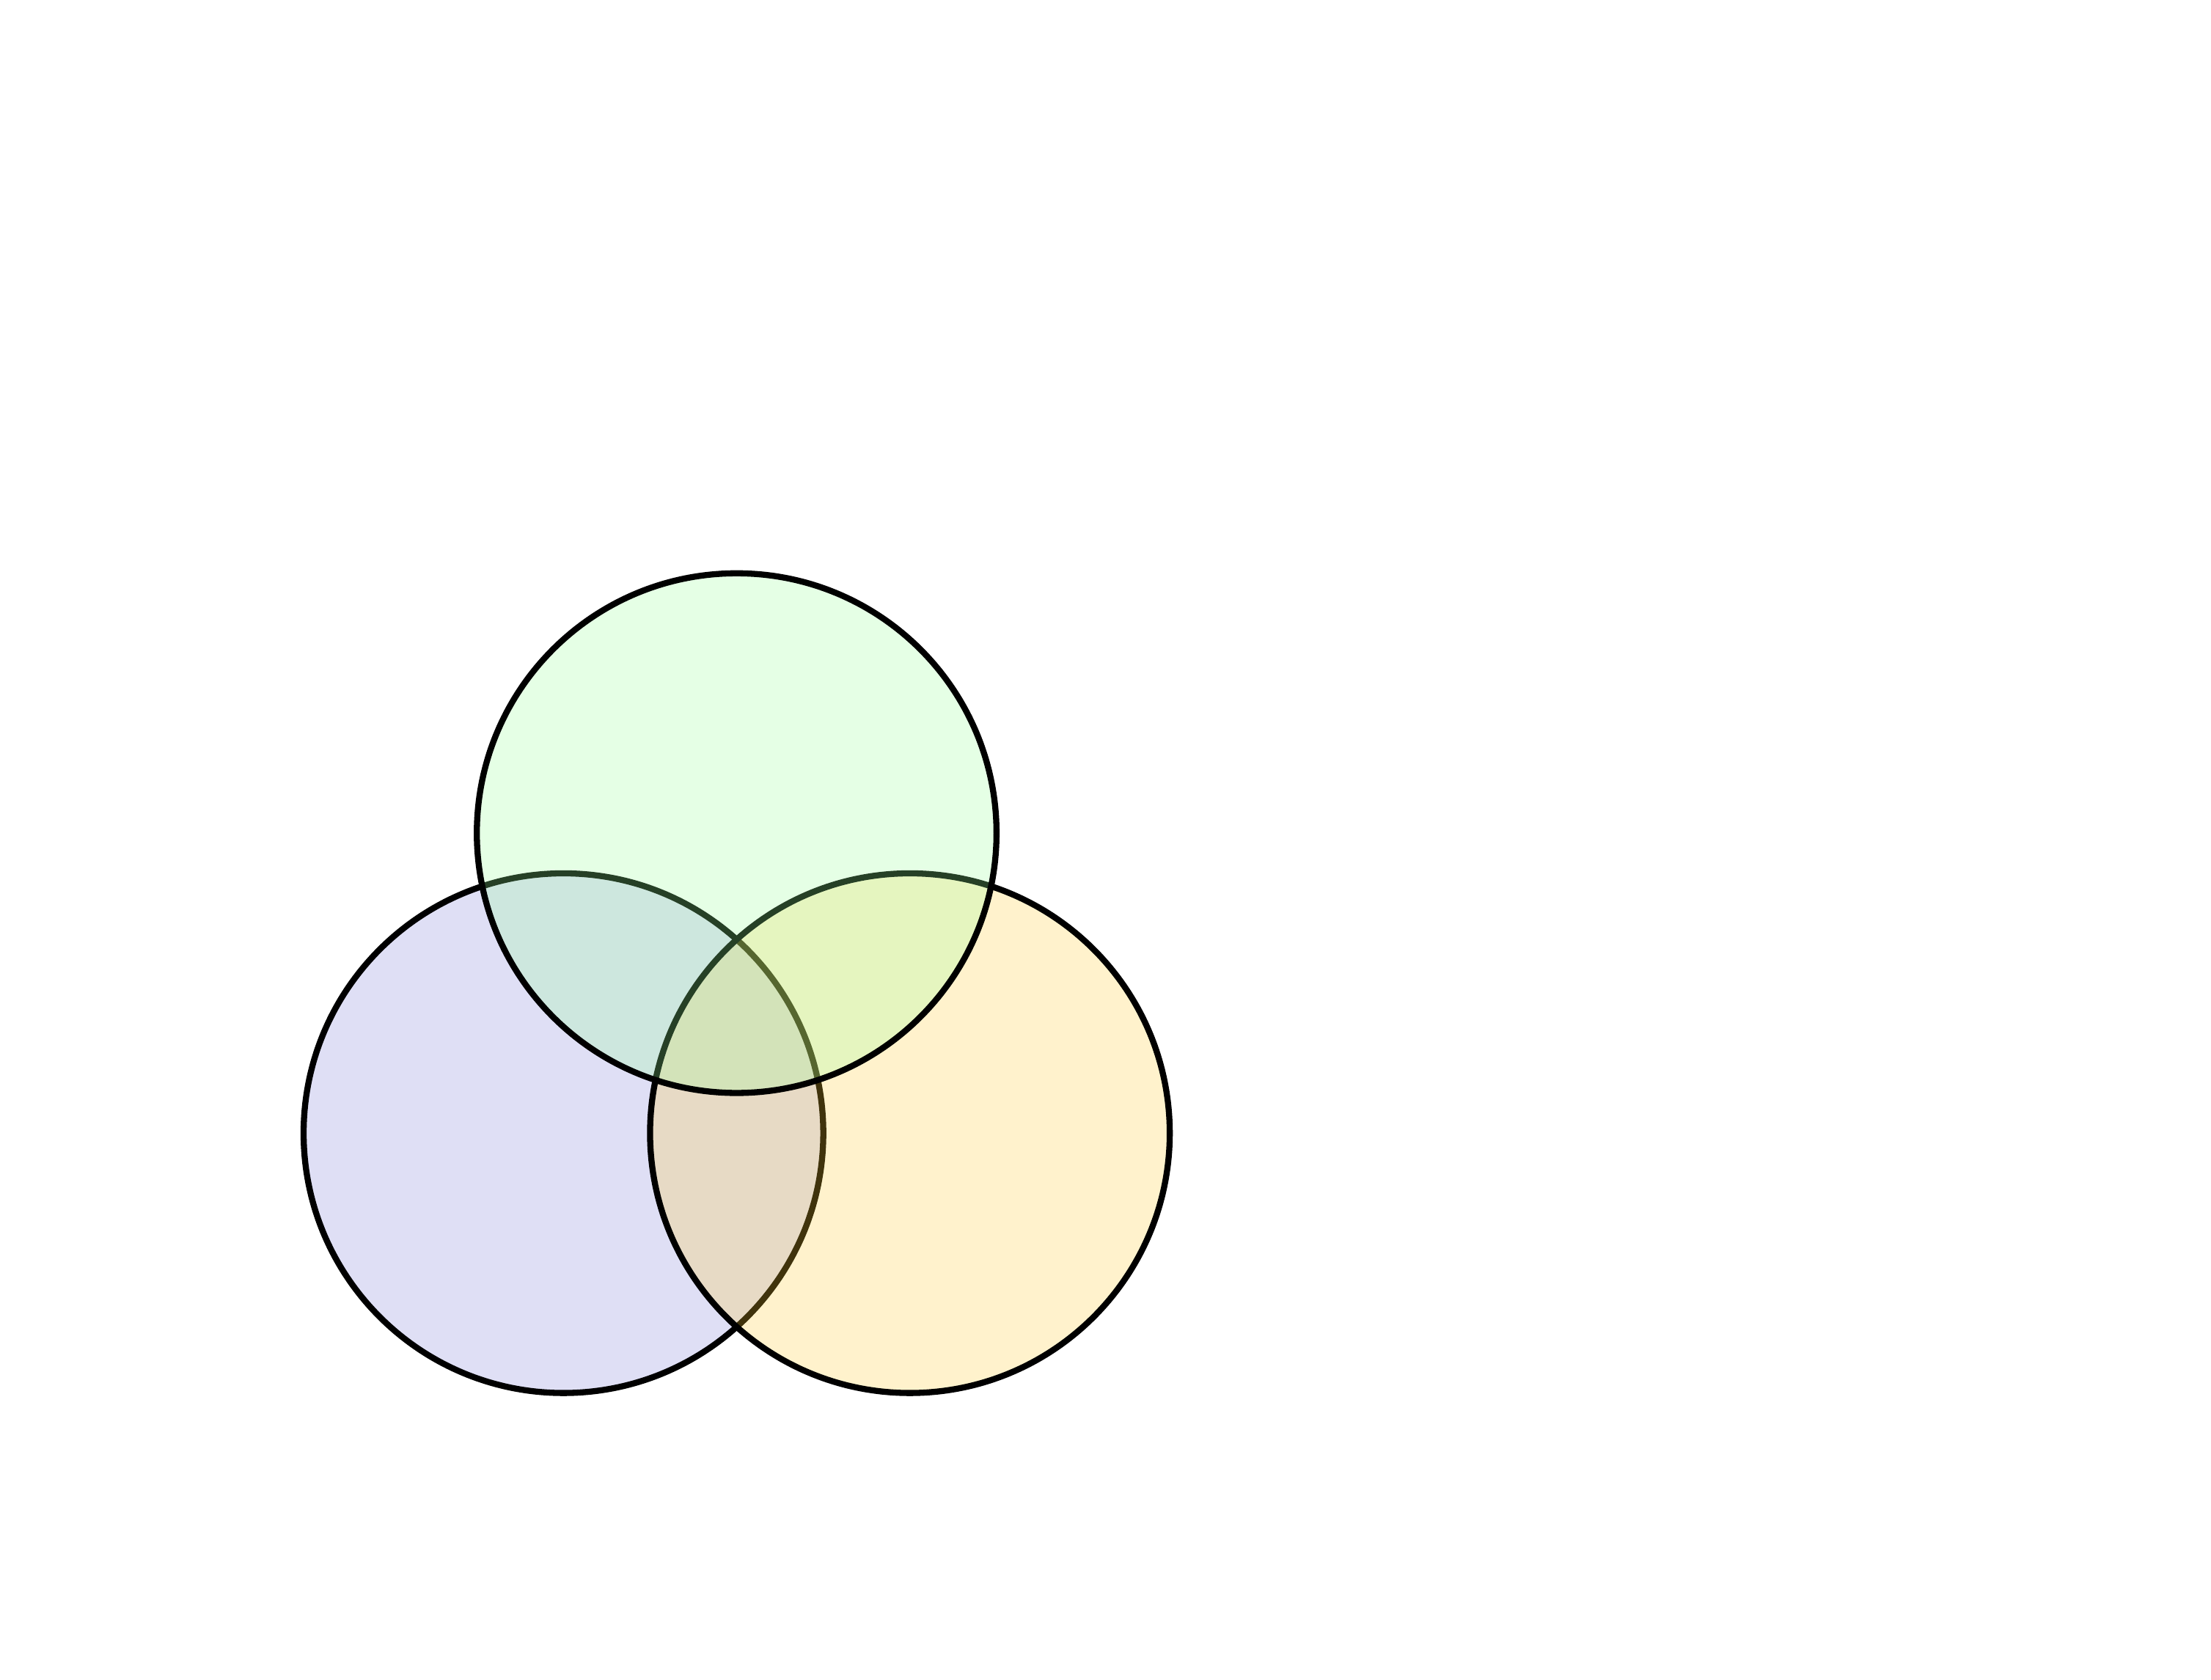
\includegraphics{introTextbookTemplate_files/figure-latex/example-1.png}
\caption{\label{fig:example}Funky tikz}
\end{figure}

After index.Rmd, bookdown loads subsequent Rmd files in alphanumeric order, so 01 comes before 02, etc

Here we have a chapter, we can have sections that are just like standard markdown

I'm not sure how to load css classes yet, but it can't be that hard

\hypertarget{ch1_s1}{%
\section{Evidence-based Research}\label{ch1_s1}}

Dr.~Anne Ecdote bases all her decisions off things she's observed. Dr.~Eva Dense bases her practice off well researched studies. Dr.~Opi Yon bases his practice off his personal beliefs. You visit each doctor with a headache. Dr.~Ecdote says the last person she saw with a headache had a brain tumor, so you should probably get an MRI. Dr.~Yon says headaches are a construct of our imagination and that if you would just stop thinking about it, it would go away. Dr.~Dense recommends a pain reliever that has been studied in several large clinical trials and repeatdtly shown to be effective at reducing headaches.

There are many definitions of statistics:
1) the science of learning from experiences
2) the science of uncertainty
To make evidence-based conclusions, we need to collect, process, analyze, and interpret data in order to draw conclusions in an objective manner.

\hypertarget{ch1_s2}{%
\section{Scientific Method}\label{ch1_s2}}

In principle, people collect and process information every day of their lives. Since it's something we do frequently, you might think we would be really good at it\ldots but we're not. Unfortunately, humans are not natural statisticians. We are not good at picking out patterns from a sea of noisy data. And, on the flip side, we are \emph{too good} at picking out non-existent patterns from small numbers of observations. We also find it difficult to sort out the effects of multiple factors occurring simultaneously and we are subject to all sorts of biases depending on our personalities, emotions, and past experiences.

Some examples of these would be good.

The \textbf{scientific method} is the process used to answer scientific questions.

\begin{enumerate}
\def\labelenumi{\arabic{enumi})}
\tightlist
\item
  Ask a question
\item
  Do background research
\item
  Construct a hypothesis
\item
  Test your hypothesis with a study or an experiment
\item
  Analyze data and draw conclusions
\item
  How do the results align with your hypothesis?
\item
  Communicate results
\end{enumerate}

learn more statistics \href{https://google.com}{here}

\hypertarget{ch1_s3}{%
\section{Introduction to Biostatistics}\label{ch1_s3}}

Biostatitsics pertains to statistics as applied to medical, biological, and health sciences. In these fields, we must often make decisions in the presence of uncertainty:

\begin{itemize}
\tightlist
\item
  Which drug should a doctor prescribe to treat an illness?\\
\item
  Can we predict the logevity of the national population to inform government decisions regarding Social Security?\\
\item
  What factors increase the risk of an individual developing coronary heart disease?
\end{itemize}

These questions are too important to be left to opinion, superstition, and conjecture. Thus, there has been a tremendous push for objective, \emph{evidence-based} decision making in medicine, public health, and policy making. Statistics is the science that allows us to make these decisions. Much of statistics was developed in the context of agricultural students, where every aspect of a plant's life can be controlled. We can create different plots of land, each with a different fertilizer, soil, sun-exposure, water, etc. and plan the same seed in each plot. Studies of humans are quite different. We can't control every aspect of a person's life, such as what they eat or where they work (no matter how great it would be for scientific purposes). There are ethical considerations - if we wanted to research the effects of smoking on lung cancer, we would not be able to force people to smoke (or not). Humans are also incredibly diverse and variable, not to mention expensive to perform research upon. Despite these issues, there is a moral imperative to make decisions on potentially life-saving therapies as fast as possible. For these reasons, biostatistics has emerged as an important field within statistics.

\hypertarget{ch1_s4}{%
\section{Statistical framework}\label{ch1_s4}}

There are three basic questions in statistics:

\begin{enumerate}
\def\labelenumi{\arabic{enumi})}
\tightlist
\item
  How should I collect my data?\\
\item
  How should I describe and summarize the data I've collected?
\item
  What does my data tell me about the way the world works?
\end{enumerate}

Throughout the book, we will cover different ways of analyzing data and making conclusions about the way the world works. Depending on the type of data, there are different methods of analysis.

In general, scientists use the scientific method to make generalizations about classes of people on the basis of their studies. The class of people that they are trying to make generalizations about is called the \textbf{population}. Most of the time, it is impratical and expensive to study all individuals in a population - although the United States government does do the best they can every 10 years. Instead of sampling everyone in the population, or taking a \textbf{census}, typically we study only a portion of th the population called the \textbf{sample}. In order to determine how best to obtain a sample to answer the research questions, we must be cautious about the \textbf{study design}. Then, researchers make generalizations, or \textbf{inference}, about the entire population based on studying the sample. We can visualize the statistical framework using this diagram:

\begin{figure}
\centering
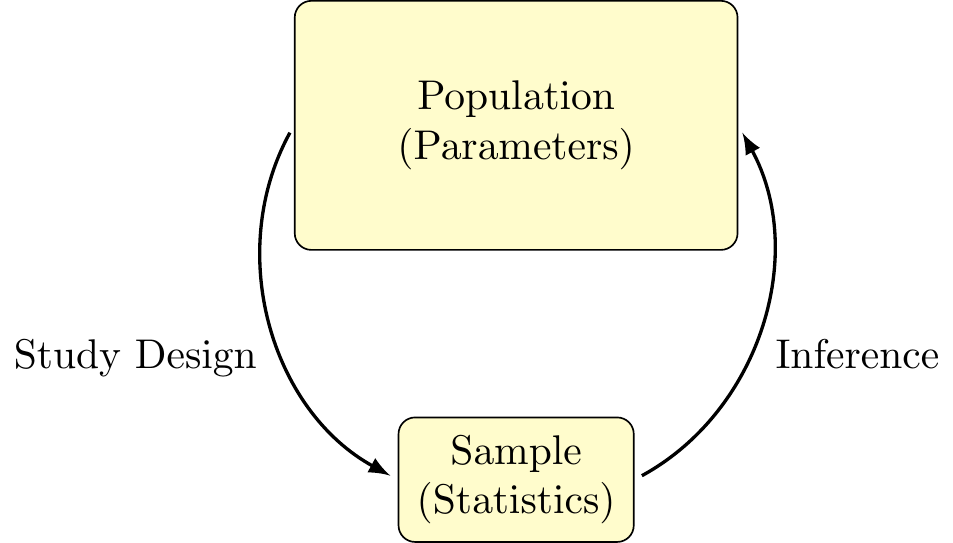
\includegraphics{introTextbookTemplate_files/figure-latex/statFramework-1.png}
\caption{\label{fig:statFramework}Statistical Framework}
\end{figure}

\hypertarget{ch1_s5}{%
\section{What is a simulation?}\label{ch1_s5}}

Many times in this book, we will illustrate or investigate a concept with a \textbf{simulation}. A simulation is a computer generated experiment where the user gets to specify the true mechanism for generating data. For example, we \emph{could} flip a fair coin over and over again and record whether each flip results in heads or tails. OR, we could tell a computer to simulate a pre-specified number of flips with the probability of heads being 50\% and get our results in a fraction of a second.

\begin{Shaded}
\begin{Highlighting}[]
\NormalTok{flipCoin }\OtherTok{\textless{}{-}} \ControlFlowTok{function}\NormalTok{(nFlips) \{}
\NormalTok{    dat }\OtherTok{\textless{}{-}} \FunctionTok{rbinom}\NormalTok{(nFlips, }\DecValTok{1}\NormalTok{, }\FloatTok{0.5}\NormalTok{)}
\NormalTok{    dat }\OtherTok{\textless{}{-}} \FunctionTok{ifelse}\NormalTok{(dat }\SpecialCharTok{==} \DecValTok{1}\NormalTok{, }\StringTok{\textquotesingle{}Heads\textquotesingle{}}\NormalTok{, }\StringTok{\textquotesingle{}Tails\textquotesingle{}}\NormalTok{)}
\NormalTok{    dat}
\NormalTok{\}}
\FunctionTok{flipCoin}\NormalTok{(}\DecValTok{5}\NormalTok{)}
\end{Highlighting}
\end{Shaded}

\begin{verbatim}
## [1] "Heads" "Tails" "Tails" "Tails" "Heads"
\end{verbatim}

Simulations are great tools for understanding the concept of randomness. For example, every time we simulate coin flips using the tool above, we will get a different data set:

\begin{Shaded}
\begin{Highlighting}[]
\FunctionTok{flipCoin}\NormalTok{(}\DecValTok{5}\NormalTok{)}
\end{Highlighting}
\end{Shaded}

\begin{verbatim}
## [1] "Heads" "Heads" "Heads" "Heads" "Heads"
\end{verbatim}

\begin{Shaded}
\begin{Highlighting}[]
\FunctionTok{flipCoin}\NormalTok{(}\DecValTok{5}\NormalTok{)}
\end{Highlighting}
\end{Shaded}

\begin{verbatim}
## [1] "Tails" "Heads" "Tails" "Heads" "Heads"
\end{verbatim}

\begin{Shaded}
\begin{Highlighting}[]
\FunctionTok{flipCoin}\NormalTok{(}\DecValTok{5}\NormalTok{)}
\end{Highlighting}
\end{Shaded}

\begin{verbatim}
## [1] "Heads" "Heads" "Tails" "Tails" "Heads"
\end{verbatim}

\begin{Shaded}
\begin{Highlighting}[]
\FunctionTok{flipCoin}\NormalTok{(}\DecValTok{5}\NormalTok{)}
\end{Highlighting}
\end{Shaded}

\begin{verbatim}
## [1] "Heads" "Heads" "Heads" "Tails" "Heads"
\end{verbatim}

\begin{Shaded}
\begin{Highlighting}[]
\FunctionTok{flipCoin}\NormalTok{(}\DecValTok{5}\NormalTok{)}
\end{Highlighting}
\end{Shaded}

\begin{verbatim}
## [1] "Tails" "Tails" "Heads" "Heads" "Tails"
\end{verbatim}

This is exactly what happens when scientists conduct a research study. If they were carry out a study in exactly the same way - sampling individuals from the same population and measuring the same quantities, they would get different results every time. This is because while each sample is from the same population, each sample will contain different individuals. Each sample is random!

\hypertarget{ch2}{%
\chapter{What is Data?}\label{ch2}}

\begin{quote}
``Numerical quantities focus on expected values, graphical summaries on unexpected values.''

--- John Tukey
\end{quote}

There are two main branches of statistics: \textbf{descriptive statistics}, which deals with methods for summarizing and/or presenting data and \textbf{inferential statistics}, which deals with methods for making generalizations about a population based on information in the sample. In this chapter, we will be focused on descriptive statistics using both numerical and graphical summaries.

\hypertarget{outline}{%
\section{Outline}\label{outline}}

\begin{itemize}
\tightlist
\item
  Introduction
\item
  Summaries (this maybe unnecessary?)

  \begin{itemize}
  \tightlist
  \item
    What is a plot/figure?
  \item
    What is a table?
  \end{itemize}
\item
  Types of Data

  \begin{itemize}
  \tightlist
  \item
    Categorical
  \item
    Continuous
  \end{itemize}
\item
  Categorical

  \begin{itemize}
  \tightlist
  \item
    visual summary
  \item
    numerical summary
  \end{itemize}
\item
  Continuous

  \begin{itemize}
  \tightlist
  \item
    Visual summary
  \item
    Numerical Summary
  \end{itemize}
\item
  Summary of Info
\end{itemize}

Headers in this document need a LOT of work

Data can be virtually anything that can be observed and recorded, including how tall you are, the number of cars of any color in town, or how many words are in each of the books in the library of congress. Just as the different types of data can vary considerably, so can the amount of data, ranging from a single number (your height) to gigabytes of data (number of words in all books definitely can't be much larger than a few Mb, so maybe a better example). As the size of the data increases, so does the difficulty of making sense of it in raw form. We can condense large quantities of data into human readable forms through the use of \textbf{data summaries}, often displayed in the forms of \textbf{tables} and \textbf{figures}. However, in doing so, information can often be lost in the process. A good data summary will seek to strike a balance between clarity and completeness of information.

\hypertarget{summaries}{%
\subsection{Summaries}\label{summaries}}

\hypertarget{types-of-data}{%
\section{Types of Data}\label{types-of-data}}

Before getting too far into the weeds, let's consider the two broad types of data that we may see in the wild, which we will call \textbf{Categorical data} and \textbf{Continuous data}.

First up is \textbf{Categorical data} (also known as \textbf{Qualitative or Discrete data}) which, as the name suggets, is data that falls into discrete categories. Categorical data can further be classified into two distinct types:

\begin{itemize}
\item
  \textbf{Nominal data}: data that exists without any sort of natural or apparent ordering, e.g., colors (red, green, blue), gender (male, female), and type of motor vehicle (car, truck, SUV).
\item
  \textbf{Ordinal data}: data that does have a natural ordering, e.g., education (high school, some college, college) and injury severity (low, medium, high)
\end{itemize}

\textbf{Continuous data}, on the other hand, is data that can be any numeric value on some interval or on a continuum. This generally includes things that can be measured quantitatively, such as height, weight, and temperature.

(Any sort of tie-in between bar charts and histograms? I.e., the discretizing of an interval? I would think not)

Different types of data can be summarized in a number of ways, which we'll explore in the next section.

\hypertarget{categorical-data}{%
\section{Categorical Data}\label{categorical-data}}

\begin{itemize}
\item
  Titanic dataset might also be good here? \textless- probably too complicated. In fact, we should probably reduce the dataset below to make it simpler
\item
  I am also wondering if I should not rearrange the order in which this is presented? That is, maybe we should start with plots rather than tables. For categorical data, leading with either seems fine, but for continuous data, plots seem far more intuitive to begin with, and numerical summaries coming next
\end{itemize}

Let's begin by considering a dataset of survey responses for 592 students responding with their hair color, eye color, and sex. This dataset includes responses from male and female students, with hair colors that are black, brown, red, and blond, and eyes that are brown, blue, hazel, and green. Note that these are \emph{qualitative} measures, suggesting that are dealing with \textbf{categorical data}.

Trying to make sense of 592 observations is a daunting task, so we can being by taking the data we have and \emph{summarizing} it in a useful way. For \textbf{categorical data}, this is often as simple as counting the number of times an observation falls into a category. For example, how many observations were male with brown hair and green eyes? Or females with red hair and blue eyes?

Let's take a look at this dataset with pairs counted together in the \texttt{Freq} column:

\begin{Shaded}
\begin{Highlighting}[]
\FunctionTok{library}\NormalTok{(knitr)}
\FunctionTok{data}\NormalTok{(HairEyeColor)}
\NormalTok{haireyecolor }\OtherTok{\textless{}{-}} \FunctionTok{as.data.frame}\NormalTok{(HairEyeColor)}
\NormalTok{haireyecolor}
\end{Highlighting}
\end{Shaded}

\begin{verbatim}
##     Hair   Eye    Sex Freq
## 1  Black Brown   Male   32
## 2  Brown Brown   Male   53
## 3    Red Brown   Male   10
## 4  Blond Brown   Male    3
## 5  Black  Blue   Male   11
## 6  Brown  Blue   Male   50
## 7    Red  Blue   Male   10
## 8  Blond  Blue   Male   30
## 9  Black Hazel   Male   10
## 10 Brown Hazel   Male   25
## 11   Red Hazel   Male    7
## 12 Blond Hazel   Male    5
## 13 Black Green   Male    3
## 14 Brown Green   Male   15
## 15   Red Green   Male    7
## 16 Blond Green   Male    8
## 17 Black Brown Female   36
## 18 Brown Brown Female   66
## 19   Red Brown Female   16
## 20 Blond Brown Female    4
## 21 Black  Blue Female    9
## 22 Brown  Blue Female   34
## 23   Red  Blue Female    7
## 24 Blond  Blue Female   64
## 25 Black Hazel Female    5
## 26 Brown Hazel Female   29
## 27   Red Hazel Female    7
## 28 Blond Hazel Female    5
## 29 Black Green Female    2
## 30 Brown Green Female   14
## 31   Red Green Female    7
## 32 Blond Green Female    8
\end{verbatim}

\begin{Shaded}
\begin{Highlighting}[]
\DocumentationTok{\#\# Gross way of doing this}
\NormalTok{dt }\OtherTok{\textless{}{-}} \FunctionTok{data.frame}\NormalTok{(}\AttributeTok{Hair =} \ConstantTok{NA}\NormalTok{, }\AttributeTok{Eye =} \ConstantTok{NA}\NormalTok{, }\AttributeTok{Sex =} \ConstantTok{NA}\NormalTok{, }\AttributeTok{Freq =} \ConstantTok{NA}\NormalTok{)}
\NormalTok{j }\OtherTok{\textless{}{-}} \DecValTok{1}
\ControlFlowTok{for}\NormalTok{(i }\ControlFlowTok{in} \FunctionTok{seq\_len}\NormalTok{(}\FunctionTok{nrow}\NormalTok{(haireyecolor))) \{}
\NormalTok{  freq }\OtherTok{\textless{}{-}}\NormalTok{ haireyecolor[i, }\StringTok{"Freq"}\NormalTok{]}
  \ControlFlowTok{for}\NormalTok{(k }\ControlFlowTok{in} \FunctionTok{seq\_len}\NormalTok{(freq)) \{}
\NormalTok{    dt[j, ] }\OtherTok{\textless{}{-}}\NormalTok{ haireyecolor[i, ]}
\NormalTok{    j }\OtherTok{\textless{}{-}}\NormalTok{ j }\SpecialCharTok{+} \DecValTok{1}
\NormalTok{  \}}
\NormalTok{\}}
\NormalTok{dt}\SpecialCharTok{$}\NormalTok{Freq }\OtherTok{\textless{}{-}} \ConstantTok{NULL}
\FunctionTok{nrow}\NormalTok{(dt)}
\end{Highlighting}
\end{Shaded}

\begin{verbatim}
## [1] 592
\end{verbatim}

By simply adding like values together, we have reduced 592 observations into 32 data points, indicating that pairing of sex, hair and eye color, as well as the number of subjects with each. Note here that in this summary of the data, no data/information was lost. That is, with these 32 rows, we could just as easily expand this out to having one row for each observation, with the number indicated in the \texttt{Freq} column.

Something about how summarizing data doesn't \emph{always} preserve everything.

Suppose first we are only interested in a portion of this data, that is, we are only interested in asking questions about hair color. The first thing we might do, then, is count how many of each hair color was observed in our dataset

\begin{Shaded}
\begin{Highlighting}[]
\CommentTok{\# hair \textless{}{-} dt$Hair}
\CommentTok{\# eye \textless{}{-} dt$Eye}
\CommentTok{\# sex \textless{}{-} dt$Sex}
\CommentTok{\# why does rmarkdown insist on pissing me off always?}
\NormalTok{tab }\OtherTok{\textless{}{-}} \FunctionTok{table}\NormalTok{(dt}\SpecialCharTok{$}\NormalTok{Hair)}
\NormalTok{nn }\OtherTok{\textless{}{-}} \FunctionTok{names}\NormalTok{(tab)}
\NormalTok{tab }\OtherTok{\textless{}{-}} \FunctionTok{as.numeric}\NormalTok{(tab)}
\FunctionTok{names}\NormalTok{(tab) }\OtherTok{\textless{}{-}}\NormalTok{ nn}
\NormalTok{tab}
\end{Highlighting}
\end{Shaded}

\begin{verbatim}
##   1   2   3   4 
## 108 286  71 127
\end{verbatim}

This kind of counting is known as \textbf{absolute frequency}, which gives us a single value indicating the total number of observations. In looking at the table above, it is clear that there are far more observations with brown hair than black, blond, and red. We gather this information by looking at the total number of observations with brown hair, and noticing that this number is quite a bit larger than any of the other observations.

However, suppose somebody asks you how common brown hair is relative to others. Does it make sense to response ``Oh, there are 286 individuals with brown hair?'' Without knowing the values for the other hair colors, this number alone doesn't carry much meaning. Is 286 observations a lot? It depends. Were 300 people examined? 3,000? Without knowing anything about the rest of the data, the absolute frequency may not be very useful.

In addition to actual counts of observations in categorical data, we may often be interested in \textbf{rates}. A rate can be as simple as taking the total number of a single category observed, and stating it in terms of the total number of observations. For example, instead of simplying saying ``286 subjects who were observed had brown hair,'' we might instead say ``286 of 592 subjects examined had brown hair.''

Perhaps more familiar to use is a \textbf{percentage}, also known as a \textbf{proportion}, which is a special type of rate, specified as the number of instances per 100 observations. We determine this by evaluating the rate with division. That is, 286 of 592 subjects becomes \(286/592 = 0.4831 = 48.31\%\). We can now show the same table above, in terms of percentages

\begin{Shaded}
\begin{Highlighting}[]
\FunctionTok{prop.table}\NormalTok{(tab)}
\end{Highlighting}
\end{Shaded}

\begin{verbatim}
##       1       2       3       4 
## 0.18243 0.48311 0.11993 0.21453
\end{verbatim}

By considering all observations as rates per one hundred, we can quickly compare the relative counts of our observations. For example, we can quickly note that about half of the observations collected had brown hair, and almost twice as many had blond hair compared to red. This kind of counting, as opposted to the raw numbers, is known as \textbf{relative frequency}.

This has given us a few ways to provide numerical summaries of the data through the use of tables, but we can just as easily obtain visual summaries as well with the use of figures and plots.

For categorical data, visual summaries often come in the form of \textbf{bar plots}. Below is a demonstration of a bar plot for the absolute frequencies of hair color found above

\begin{Shaded}
\begin{Highlighting}[]
\FunctionTok{barplot}\NormalTok{(tab, }\AttributeTok{main =} \StringTok{"Why does bookdown change hair color to numbers everywhere?"}\NormalTok{)}
\end{Highlighting}
\end{Shaded}

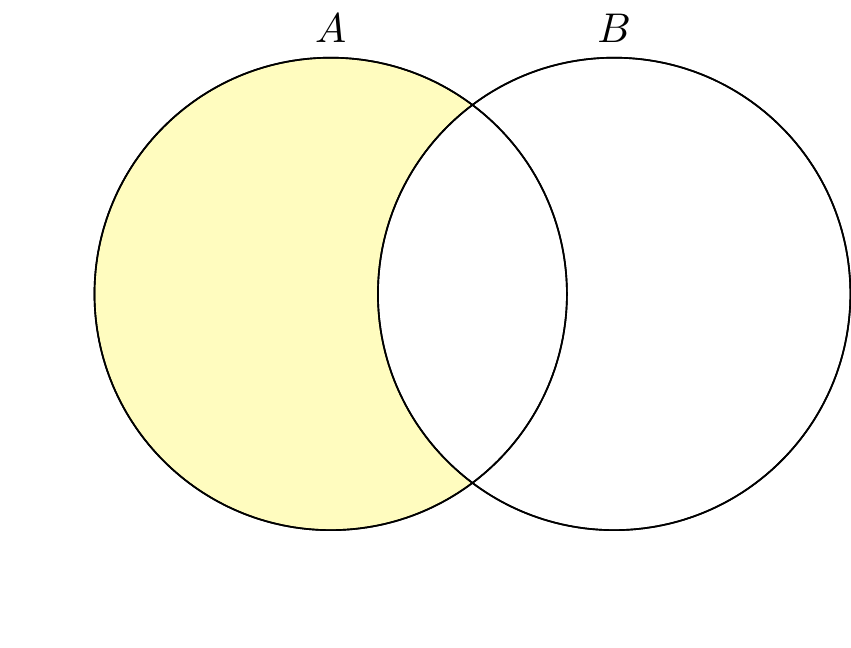
\includegraphics{introTextbookTemplate_files/figure-latex/unnamed-chunk-7-1.pdf}

\textless{} This is possibly too much info for the 2x2 tables. We can perhaps choose one margin to run with? \textgreater{}

Numerical and visual summaries become even more useful as our data becomes more complicated. Let's continue with the example we had before, but now let us also break down observations with each hair color by eye color as well. This process is known as \textbf{stratification}

\begin{Shaded}
\begin{Highlighting}[]
\NormalTok{table2 }\OtherTok{\textless{}{-}} \FunctionTok{with}\NormalTok{(dt, }\FunctionTok{table}\NormalTok{(Eye, Hair))}
\NormalTok{table2}
\end{Highlighting}
\end{Shaded}

\begin{verbatim}
##    Hair
## Eye   1   2   3   4
##   1  68 119  26   7
##   2  20  84  17  94
##   3  15  54  14  10
##   4   5  29  14  16
\end{verbatim}

First, we notice that by taking sums down the columns, we arrive at the same numbers that we had when only hair color was considered. If we were to sum these numbers up, they would add to 592, the total number of observations in our dataset. In other words, we haven't lost any information related to the number of observations with each hair color, but we have \emph{added information} to our summary by including eye color as well.

One will also notice that if we sum horizontally, we get the total number of observations with each eye color as well. This is done in the margins in the table below. Note that the sum of both margin totals add up to 592, the total number of observations, as indicated by the bottom right corner.

\begin{Shaded}
\begin{Highlighting}[]
\FunctionTok{addmargins}\NormalTok{(table2)}
\end{Highlighting}
\end{Shaded}

\begin{verbatim}
##      Hair
## Eye     1   2   3   4 Sum
##   1    68 119  26   7 220
##   2    20  84  17  94 215
##   3    15  54  14  10  93
##   4     5  29  14  16  64
##   Sum 108 286  71 127 592
\end{verbatim}

Similar to our previous example, these numbers represent the \emph{absolute frequencies} of our observations.

Unlike the previous example, however, we now have several ways in which we might compute the \emph{relative frequencies}. In particular, this asks the question ``relative to what?'' For the table above, there are three ``whats'' that may be of interest

\begin{itemize}
\tightlist
\item
  How many in each category, relative to the entire population
\item
  How many in each eye color, within hair color
\item
  How many in each hair color, within eye color
\end{itemize}

I'm not sure which, if any, are relevant, so I won't write these out just yet. Also, I know, magrittr. It's just here for convienience

\begin{Shaded}
\begin{Highlighting}[]
\CommentTok{\# by population}
\FunctionTok{prop.table}\NormalTok{(table2)}
\end{Highlighting}
\end{Shaded}

\begin{verbatim}
##    Hair
## Eye         1         2         3         4
##   1 0.1148649 0.2010135 0.0439189 0.0118243
##   2 0.0337838 0.1418919 0.0287162 0.1587838
##   3 0.0253378 0.0912162 0.0236486 0.0168919
##   4 0.0084459 0.0489865 0.0236486 0.0270270
\end{verbatim}

\begin{Shaded}
\begin{Highlighting}[]
\CommentTok{\# by hair color}
\FunctionTok{prop.table}\NormalTok{(table2, }\AttributeTok{margin =} \DecValTok{2}\NormalTok{) }\SpecialCharTok{\%\textgreater{}\%} \FunctionTok{addmargins}\NormalTok{(}\DecValTok{1}\NormalTok{)}
\end{Highlighting}
\end{Shaded}

\begin{verbatim}
##      Hair
## Eye          1        2        3        4
##   1   0.629630 0.416084 0.366197 0.055118
##   2   0.185185 0.293706 0.239437 0.740157
##   3   0.138889 0.188811 0.197183 0.078740
##   4   0.046296 0.101399 0.197183 0.125984
##   Sum 1.000000 1.000000 1.000000 1.000000
\end{verbatim}

\begin{Shaded}
\begin{Highlighting}[]
\CommentTok{\# by eye color}
\FunctionTok{prop.table}\NormalTok{(table2, }\AttributeTok{margin =} \DecValTok{1}\NormalTok{) }\SpecialCharTok{\%\textgreater{}\%} \FunctionTok{addmargins}\NormalTok{(}\DecValTok{2}\NormalTok{)}
\end{Highlighting}
\end{Shaded}

\begin{verbatim}
##    Hair
## Eye        1        2        3        4      Sum
##   1 0.309091 0.540909 0.118182 0.031818 1.000000
##   2 0.093023 0.390698 0.079070 0.437209 1.000000
##   3 0.161290 0.580645 0.150538 0.107527 1.000000
##   4 0.078125 0.453125 0.218750 0.250000 1.000000
\end{verbatim}

\begin{Shaded}
\begin{Highlighting}[]
\FunctionTok{barplot}\NormalTok{(table2, }\AttributeTok{beside =} \ConstantTok{TRUE}\NormalTok{, }\AttributeTok{main =} \StringTok{"By Hair Color"}\NormalTok{)}
\end{Highlighting}
\end{Shaded}

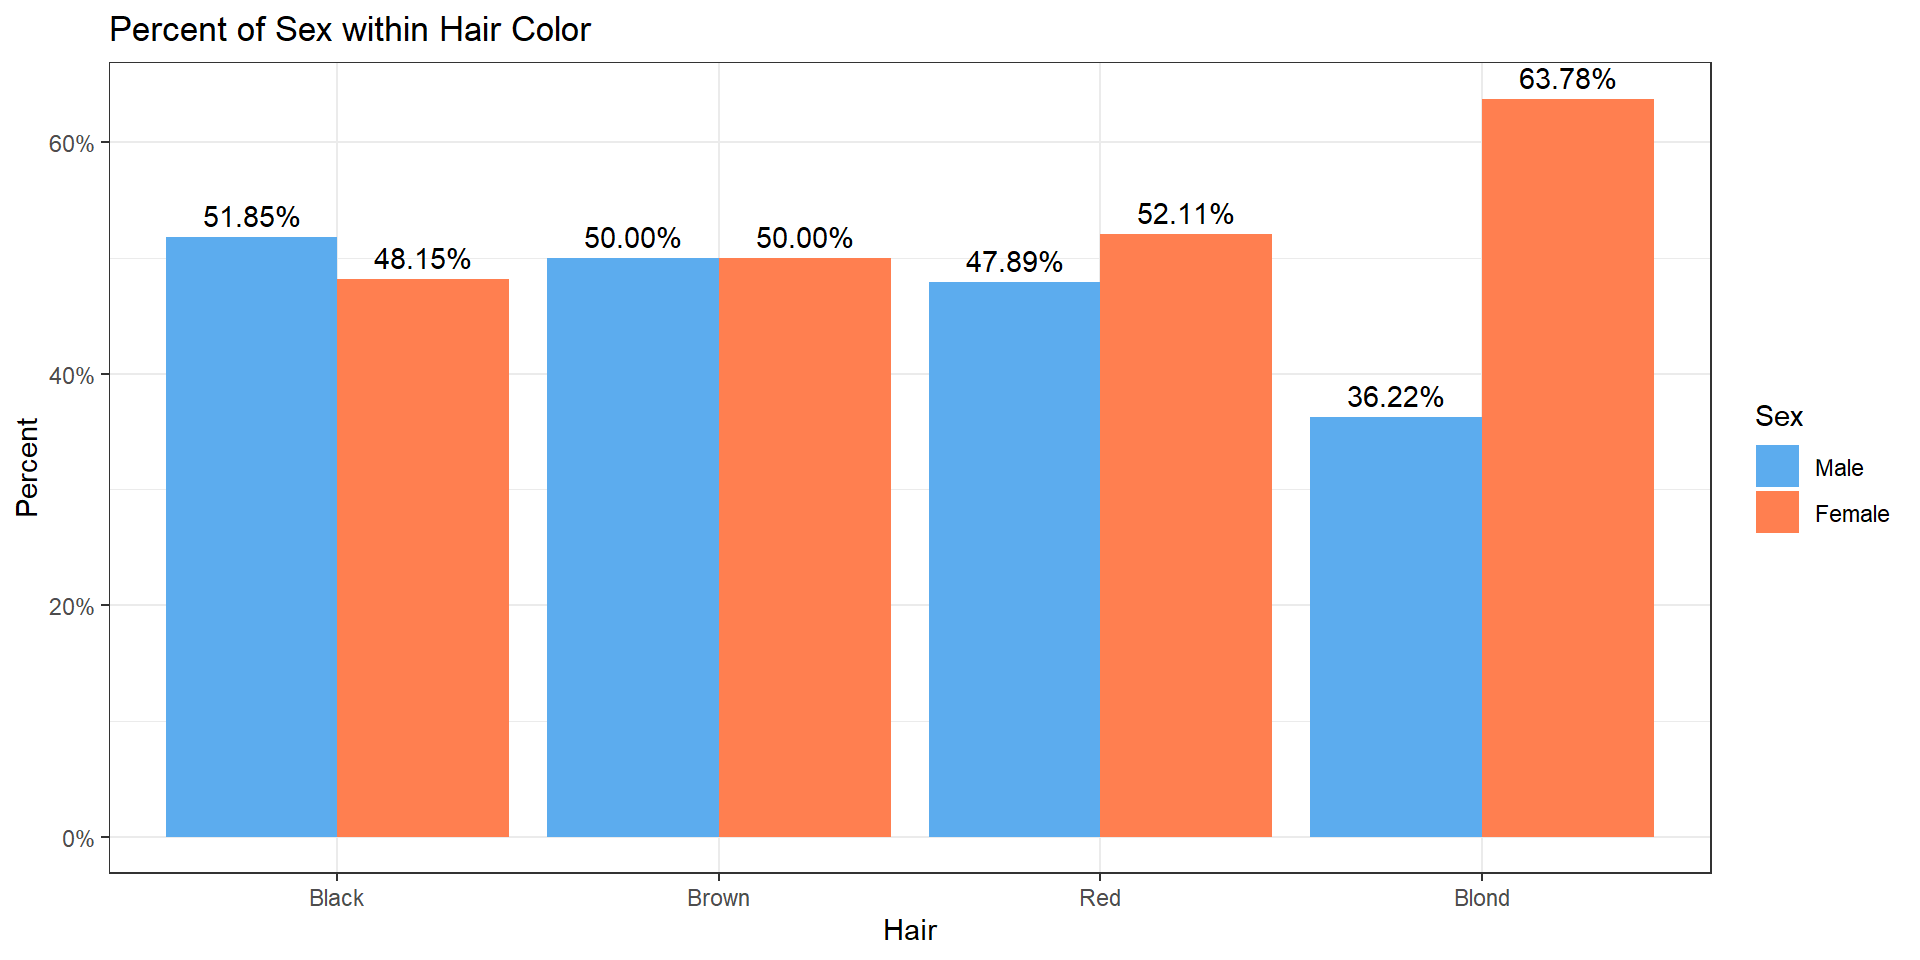
\includegraphics{introTextbookTemplate_files/figure-latex/unnamed-chunk-11-1.pdf}

\begin{Shaded}
\begin{Highlighting}[]
\FunctionTok{barplot}\NormalTok{(}\FunctionTok{t}\NormalTok{(table2), }\AttributeTok{beside =} \ConstantTok{TRUE}\NormalTok{, }\AttributeTok{main =} \StringTok{"By Eye Color"}\NormalTok{)}
\end{Highlighting}
\end{Shaded}

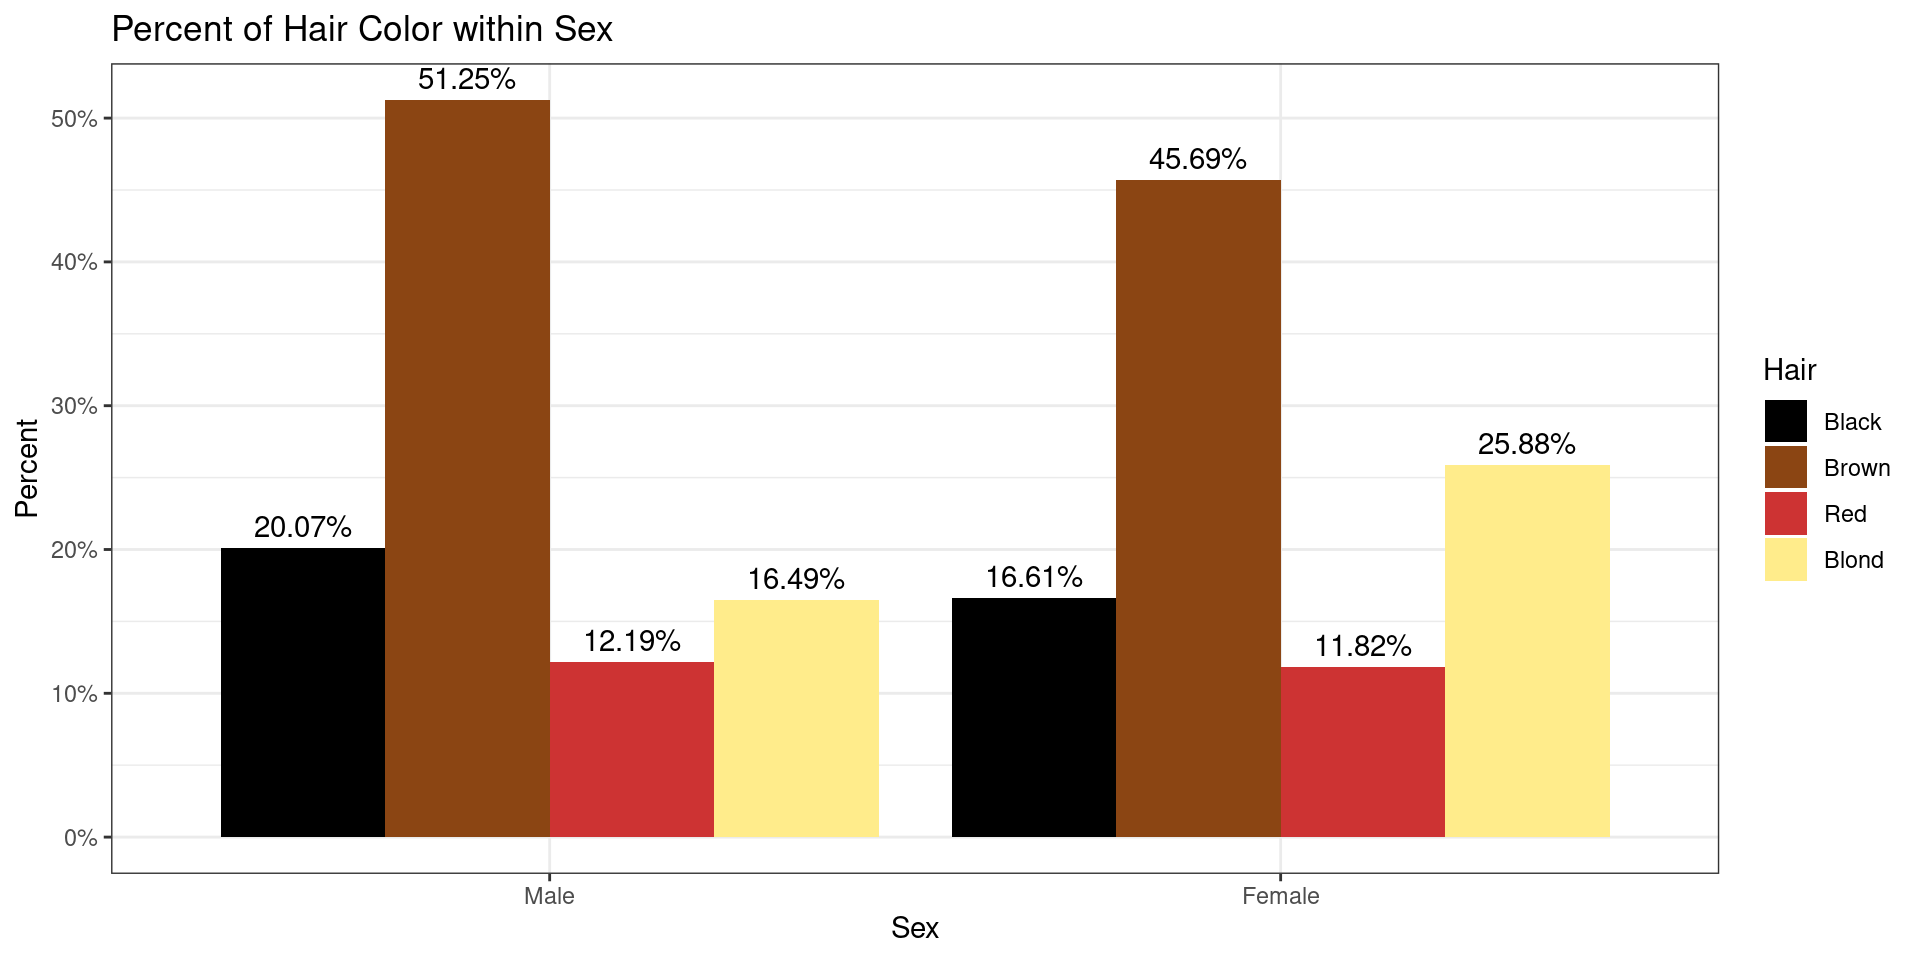
\includegraphics{introTextbookTemplate_files/figure-latex/unnamed-chunk-11-2.pdf}

Seemingly, we'll just need to go back and do everything in ggplot, because this is just ridiculous.

I feel silly mentioning mode. Probably the best way to fill in the stuff above is come up with questions and then answer them by looking at table.

It might be easier if we find something with less categories. Maybe I could do sex instead of eye color? I wish I would have thought of that before doing everything above

\hypertarget{continuous-data}{%
\section{Continuous data}\label{continuous-data}}

\begin{itemize}
\tightlist
\item
  \texttt{faithful} data cool because it's bimodal, but that also makes transition into measures of center, spread, and skewness more difficult.
\item
  Possibly not bad is \texttt{airquality} It has

  \begin{itemize}
  \tightlist
  \item
    Ozone (skew)
  \item
    Solar radiation (skew but closer to uniform)
  \item
    Wind in mph (bimodal)
  \item
    Temp (normal)
  \end{itemize}
\item
  Note: also option to not use formal data set and just use distributions to control skew
\end{itemize}

While tables of frequencies and barcharts are great for data that can be counted and categorized, it does not give us much in terms of dealing with \emph{continuous data}, which could have potentially an infinite number of different values. Like categorical date, continuous data is typically summarized in two ways:

\begin{itemize}
\tightlist
\item
  Graphical Visualizations
\item
  Numerical Summaries
\end{itemize}

Let's begin by looking at each of these in turn.

\hypertarget{graphical-summaries}{%
\subsection{Graphical Summaries}\label{graphical-summaries}}

Let's begin by considering a hypothetical dataset in which we have collected the age, in years, of 50 subjects.

\begin{Shaded}
\begin{Highlighting}[]
\DocumentationTok{\#\# Idk, I wanted something maybe not uniform? This can be changed}
\FunctionTok{set.seed}\NormalTok{(}\DecValTok{123}\NormalTok{)}
\NormalTok{age }\OtherTok{\textless{}{-}} \FunctionTok{c}\NormalTok{(}\FunctionTok{sample}\NormalTok{(}\DecValTok{20}\SpecialCharTok{:}\DecValTok{29}\NormalTok{, }\DecValTok{25}\NormalTok{, }\AttributeTok{replace =} \ConstantTok{TRUE}\NormalTok{), }\FunctionTok{sample}\NormalTok{(}\DecValTok{30}\SpecialCharTok{:}\DecValTok{60}\NormalTok{, }\DecValTok{25}\NormalTok{, }\AttributeTok{replace =} \ConstantTok{TRUE}\NormalTok{))}
\NormalTok{age}
\end{Highlighting}
\end{Shaded}

\begin{verbatim}
##  [1] 22 22 29 21 25 24 23 25 28 29 24 22 28 28 28 22 27 29 26 29 28 22 23 20 26
## [26] 50 41 44 39 42 36 38 38 39 52 56 57 50 36 50 56 35 54 31 58 34 37 41 60 42
\end{verbatim}

Now, we could consider counting the number of subjects at each age and, similar to the plots in categorical data, create a plot demonstrating what our sample looks like

\begin{Shaded}
\begin{Highlighting}[]
\FunctionTok{table}\NormalTok{(age)}
\end{Highlighting}
\end{Shaded}

\begin{verbatim}
## age
## 20 21 22 23 24 25 26 27 28 29 31 34 35 36 37 38 39 41 42 44 50 52 54 56 57 58 
##  1  1  5  2  2  2  2  1  5  4  1  1  1  2  1  2  2  2  2  1  3  1  1  2  1  1 
## 60 
##  1
\end{verbatim}

\begin{Shaded}
\begin{Highlighting}[]
\FunctionTok{barplot}\NormalTok{(}\FunctionTok{table}\NormalTok{(age))}
\end{Highlighting}
\end{Shaded}

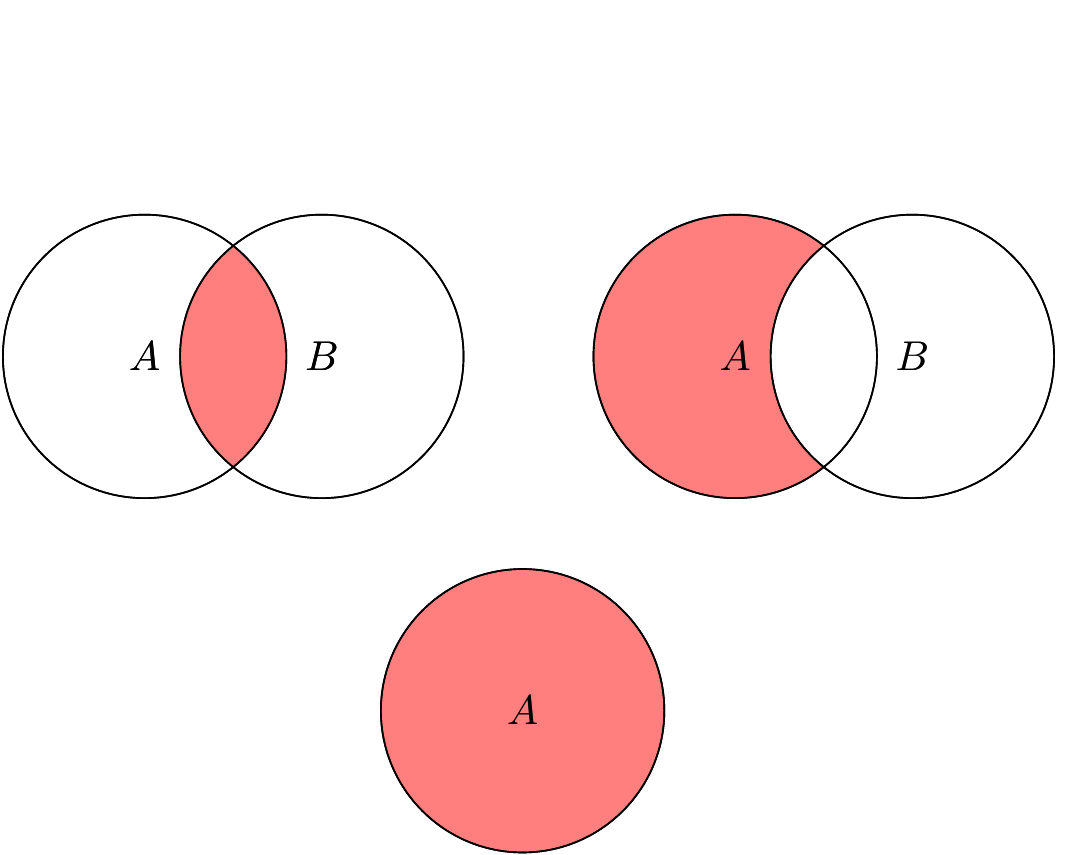
\includegraphics{introTextbookTemplate_files/figure-latex/unnamed-chunk-13-1.pdf}

While this is slightly more helpful than the raw numerical values, it's not by much. We can see that some ages are more prevelant than others, but we still have 40 separate values that we are looking at on our graph.

As an alternative, we can consider a \emph{histogram} which, similar to a barplot, aggregates values into bins. Let's look at the same data above, but now binning our observations into sets of ten years (25-34, 35-44, etc)

\begin{Shaded}
\begin{Highlighting}[]
\FunctionTok{hist}\NormalTok{(age, }\AttributeTok{breaks =} \FunctionTok{seq}\NormalTok{(}\FunctionTok{min}\NormalTok{(age), }\FunctionTok{max}\NormalTok{(age), }\AttributeTok{by =} \DecValTok{10}\NormalTok{))}
\end{Highlighting}
\end{Shaded}

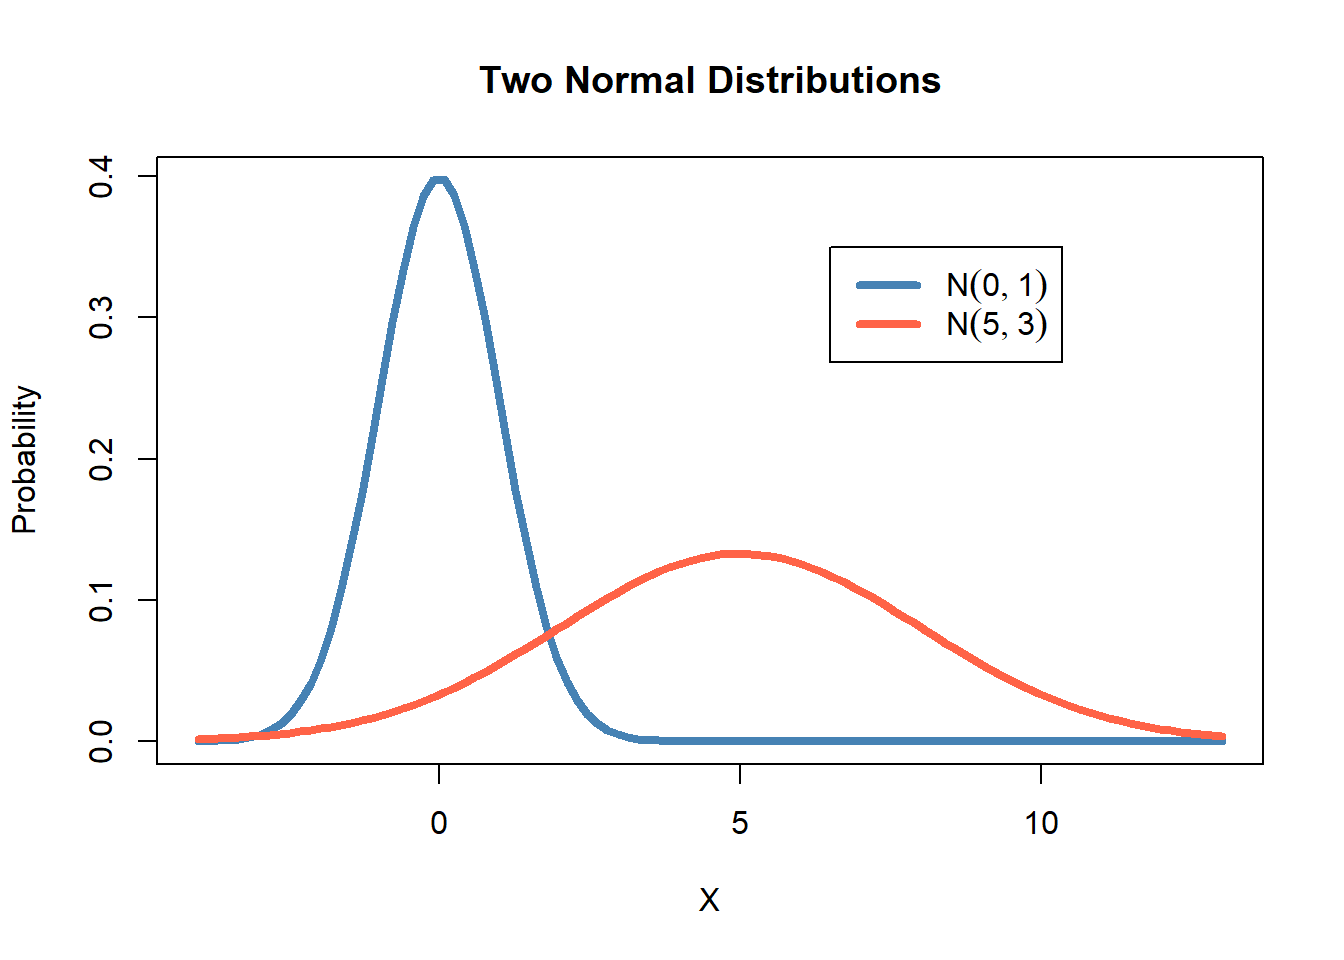
\includegraphics{introTextbookTemplate_files/figure-latex/unnamed-chunk-14-1.pdf}

Notice how this paints a slightly different picture than the barplot above. Whereas the first plot gave us counts for each individual age, the histogram gives us a \emph{graphical summary} of the ages, indicating the number of subjects in each decade. From this histogram, then, we quickly see that there are far more subjects in the 20-29 range, than each of the others. We may have come to a similar conclusion looking at the original bar chart. However, what we also see here is that the number of subject in the 30-39 range is larger and 40-49, and so on. An observation like this is not as immediately avaiable when looking at the original bar chart.

\hypertarget{numerical-summaries}{%
\subsection{Numerical Summaries}\label{numerical-summaries}}

While looking at a graphical summary can often give us quick insight into patterns in our data, the use of \emph{numerical summaries} can allow us to be much more precise. Typically with continuous data, we can reduce all of the data to a few numerical values that describe the data in detail. These include:

\begin{itemize}
\tightlist
\item
  Center
\item
  Spread
\item
  Skewness
\end{itemize}

We look at each of these in turn

\hypertarget{center}{%
\subsubsection{Center}\label{center}}

Numbers designed to reflect the center of a dataset are called \emph{Measures of Central Tendancy}. There are three popular arithmetic measures used to caputre the center of a ((distribution)), namely

\begin{itemize}
\tightlist
\item
  Mean
\item
  Median
\item
  Mode
\end{itemize}

Before moving onto these in detail, let's take a moment for a brief review of Summation Notation (((Would be cool to have a div element for ``Review'' or ``Btw.'' We could also include an appendix where all of this is explained in more detail that they can click to visit, with an actual ``quick review'' done here)))

\begin{center}\rule{0.5\linewidth}{0.5pt}\end{center}

{[}{[}Probably ought to start with N then move to n{]}{]}

In general, we will let lowercase \(n\) represent the total number of observations that we have collected. We can express these observations as

\[
x_1, x_2, \dots, x_n
\]
where the subscript values are used to identify each observation. We can represent the sum of all of these observations using the abbreviated \emph{Sigma} notation,

\[
x_1 + x_2 + \dots + x_n = \sum_{i=1}^n x_i
\]
On the right hand side, note that the value of \(x\) has a subscript \(x_i\), while the Sigma notation has \(i=1\) on the bottom and \(n\) on the top. This is to indicate that we are to go through each value of \(i = 1, 2, \dots, n\), for each value of \(x_i\). In other words, where we might say \(x_1\) is the first observation, we would say that \(x_i\) is the \(i\)th observation. This is convenient when we want to describe any \(x\) value, but it is not important which one we choose.

\begin{center}\rule{0.5\linewidth}{0.5pt}\end{center}

{[}{[}Yeah, but what do we mean by `center' of a distribution?{]}{]}

The \emph{mean} is the most commonly used measure to find the center of a distribution. Simply enough, the mean can be found by taking the sum of all of the observations, and dividing by the total number. We can express this concisely in the following way

\[
\frac{x_1 + x_2 + \dots + x_n}{n} = \frac1n \sum_{i=1}^n x_i
\]
Note how this is similar to the Sigma summation expression above. Here, we are taking the sum of each \(x_i\), and then dividing this total by \(n\).

Now, in statistics, we often talk about the mean in two different ways, which we will illustrate here. Consider, for example, the case in which we want to know the mean height of each individual living in the state of Iowa. We will present the number of people in Iowa, also known as the \(population\), as \(N\). That is, there are \(N\) people living in Iowa. The mean of this entire population, known as the \emph{population mean} is designated by the Greek later \(\mu\) (called \emph{mu}). Mathematically, we would write this as

\[
\mu = \frac1N \sum_{i=1}^N x_i
\]
Now, finding the height of each person in Iowa is likely to be very difficult, if not impossible. Often, we can get a reasonable estimate of the population mean by taking a sample of people and treating them as an approximation of the entire population. This sample will represent the actual observations we collect, and we will represent this as we did above with the lower case \(n\), where generally, \(n < N\) (often by quite a bit). The \emph{sample mean}, which we denote \(\bar{x}\) (called x-bar), can be expressed similarly

\[
\bar{x} = \frac1n \sum_{i=1}^n x_i
\]
There are two major differences here between these two values that are worth giving a second consideration to

\begin{itemize}
\tightlist
\item
  The population mean has \(N\) observations, which is always larger than the \(n\) observations in the sample
\item
  While there is only one way to select \(N\) observations from \(N\) subjects, there are many ways to select \(n\) observations from \(N\) subjects. For example, if you have five different cookies, there is only one way to select all five cookies, while there are ten different ways to select only three (I know childish example, maybe we could have a picture? Though this also introduces some benefit to non-rigorous introduction of combinations, which could be useful in explaining variance in samples?)
\end{itemize}

In general, we have that \(\bar{x} \approx \mu\), with this approximation being better the closer \(n\) is to \(N\). This is a topic we will return to shortly.

\begin{center}\rule{0.5\linewidth}{0.5pt}\end{center}

Median

The \emph{median}, similar to the mean, is another common measure of the center of a distribution. In particular, for a set of observations, the median is an observed value that is both larger than half of the observations, as well as smaller than half of the observations. Formally, we say that the median is the 50th percentile of a dataset. Informally, we say it's the value in the middle (I don't like this).

To find the median, we begin by arranging our data from smallest to largest. If the total number of observations, \(n\), is odd, then the median is simply the middle observation. If \(n\) is even, it is the mean of the middle two.

Examples:

\begin{itemize}
\tightlist
\item
  \(1, 2, 2, 3, {\color{red} 5}, 7, 9, 10, 11 \quad \Rightarrow \quad \text{Median} = 5\)
\item
  \(1,2,2,3, {\color{red} 5}, {\color{red} 6}, 7, 9, 10, 11, \quad \Rightarrow \quad \text{Median} = \frac{(5+6)}{2} = 5.5\)
\end{itemize}

If both the mean and the median are both measures of central tendency, should we expect them to give us similar impressions about the center of a data set? {[}{[}Maybe we should have commentary on why we might be interested in center, somewhere near the beginning of this chapter. Like, maybe all of the high level ideas first, THEN do statistics and discrete/continuous plots?{]}{]}

Let's consider an example where we collect \(n = 10\) samples of salaries for University of Iowa employees:

{[}{[}gross table for now{]}{]}

\$31,176

\$130,000

\$50,879

\$37,876

\$34,619

\$144,600

\$103,000

\$48,962

\$36,549

\$5,075,000

With regards to salaries, we find that

\begin{itemize}
\tightlist
\item
  Mean = \$569,266
\item
  Median = (48,962 + 50,879) / 2 = \$49,921
\end{itemize}

Due to one extremely high salary in our observation, the median is a much better reflection of the typical UI salary.

This one high salary, not representative of most of the salaries collected, is known as an \textbf{outlier}. From the example above, we see that the mean is highly sensitive to the presence of outliers, while the median is not. Measures that are not sensitive to outliers are known as \textbf{robust}, or \emph{resistant}. We see, then, that the median is a robust estimator of the center of the data.

{[}{[}As mentioned above, we should maybe introduce skewness earlier?{]}{]}

We see above a case in which the mean and median are widely different, owing thanks to the outlier. This begs the broader question, when might we expect these measures of central tendancy to be the same, and when might we expect them to differ?

Below, we consider a collection of plots illustrating common ``shapes'' we might see in our data.

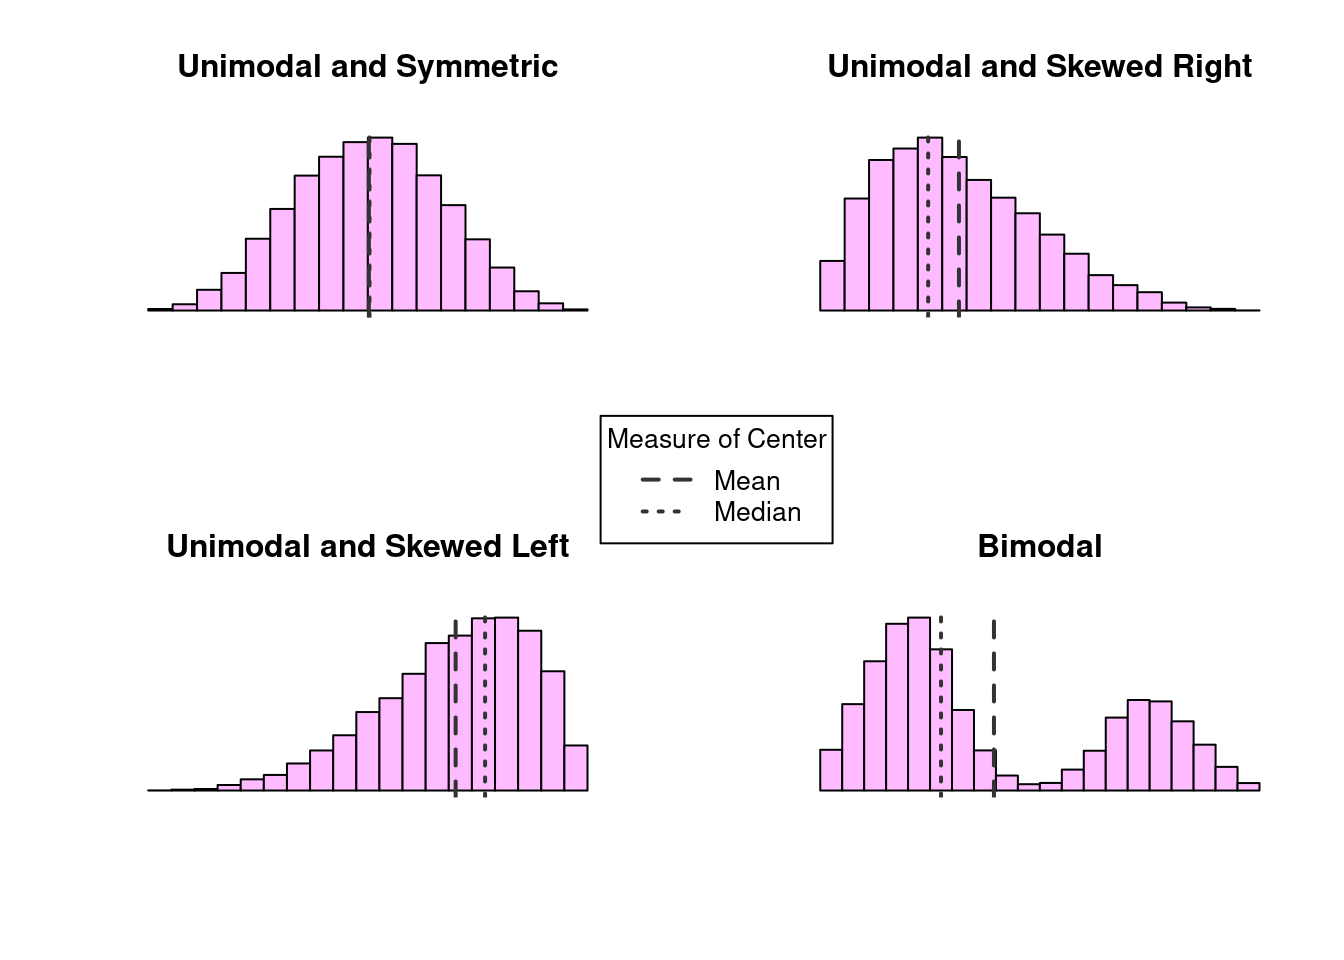
\includegraphics{introTextbookTemplate_files/figure-latex/unnamed-chunk-16-1.pdf}

{[}{[}Do we need discussion on mode? Skipping for now{]}{]}

\hypertarget{measures-of-spread}{%
\subsection{Measures of Spread}\label{measures-of-spread}}

This is just getting these on paper. Serious reorganization needs to occur

Suppose that we have two datasets, each with 1,000 observations, and each with both a common mean and median of 100:

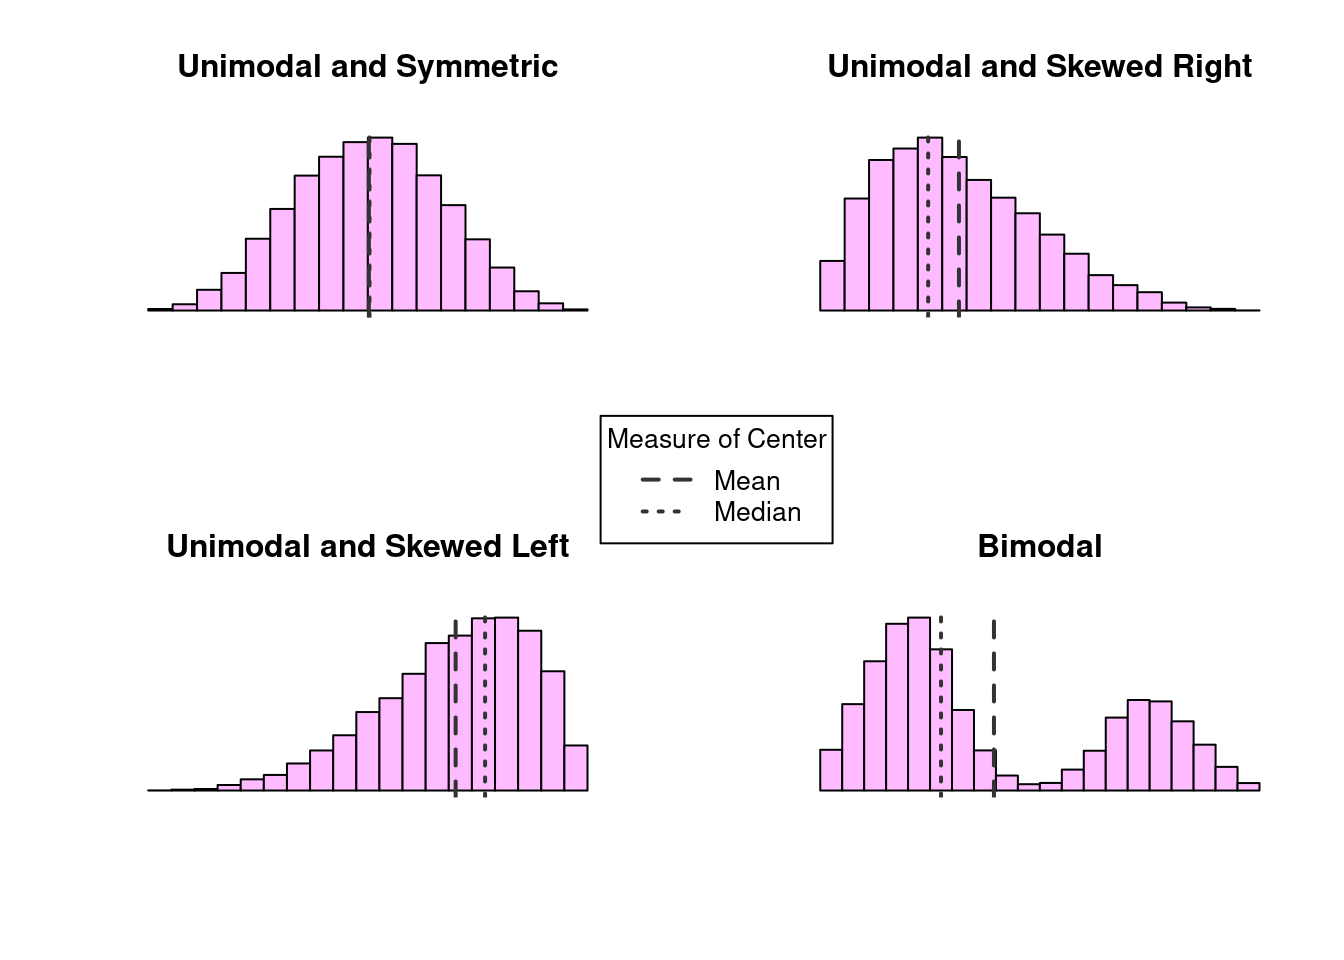
\includegraphics{introTextbookTemplate_files/figure-latex/unnamed-chunk-17-1.pdf}

From the histograms above, we visually confirm that both datasets have a mean and median of 100. Despite this, however, it would appear as if these datasets are not quite as similar as one might have thought

\begin{itemize}
\item
  First, we see that for the first dataset, nearly all of the values fall in the range of (50, 150), while for the second dataset, this range appears to be closer to (0, 200)
\item
  Recalling that each dataset has the same number of observations, it appears as if the first dataset has nearly twice as many observations near the mean value of 100 than the second dataset
\end{itemize}

Suppose, then, you are approached by a researcher who wants to select a single observation from each dataset at random, and you are asked to anticipate what value that observation will have. Without having seen them, the best guess you can offer is our measure of center, which is 100. From which dataset do you suspect the random observation will have a value closer to 100? Which do you suspect will be further away?

What we are observing here is two datasets with a common center that have different \emph{spread} or \emph{dispersion}.

Next to the center, this is the second most important piece of information informing us on the shape of our data. Roughly speaking, the spread of the data informs us of the degree to which our observations tend to lie close to the center or scattered away from it. Just as we have multiple ways to determine the center of a dataset, so we have several methods for quantifying the variability of the data. These numeric summaries are known as \emph{Measures of Dispersion}. Measures that we will investigate here include

\begin{itemize}
\tightlist
\item
  Variance
\item
  Standard deviation
\item
  Range
\item
  Interquartile Range (IQR)
\end{itemize}

\hypertarget{variance-and-standard-deviation}{%
\paragraph{Variance and Standard Deviation}\label{variance-and-standard-deviation}}

In mathematical terms, we describe the \textbf{variance} of a dataset to be \emph{the average of the squared differences between each data value and the sample mean}. The \textbf{standard deviation} is defined as the \emph{square root of the variance}.

{[}{[}something something clever way of inuiting what variance is{]}{]}
{[}{[}\url{https://assessingpsyche.wordpress.com/2014/07/10/two-visualizations-for-explaining-variance-explained/}{]}{]}

As before, consider a population with \(N\) observations denoted as

\[ 
x_1, x_2, \dots, x_N
\]
To tie into our definition, note that \((x_i - \mu)\) represents the difference between an observation and the population mean, while \((x_i - \mu)^2\) represents the squared difference. The \textbf{population variance}, defined as the average of these squared differences, is denoted as \(\sigma^2\), where

\[
\sigma^2 = \frac{1}{N} \sum_{i=1}^N (x_i - \mu)^2
\]

The \textbf{population standard deviation}, being the square root of the population variance, is denoted \(\sigma = \sqrt{\sigma^2}\).

Like our measure for the mean, we can have both a population variance, as well as a \textbf{sample variance}. That is, suppose we have a sample of \(n < N\) observations,

\[
x_1, x_2, \dots, x_n
\]
The sample variance, denoted \(s^2\), is nearly identical to the population variance, with the exception of the fact that we now subtract the sample mean, rather than the population mean

\[
s^2 = \frac{1}{n-1} \sum_{i=1}^n (x_i - \bar{x})^2
\]
Similarly, the \textbf{sample standard deviation} is written as the square root, \(s = \sqrt{s^2}\). A few things to be on the lookout for:

\begin{itemize}
\item
  See that the sample variance finds the average by multiplying by \(\frac{1}{n-1}\) rather than \(\frac1n\). This is because there is no God, and ironically, the world is doomed to end in eternal darkness after being engulfed by our only source of light, the sun
\item
  Be extra careful when finding standard deviations. It is the \emph{square root} of the sum, rather than the square root of terms inside of the sum. that is,
\end{itemize}

\[
\sigma = \sqrt{\frac{1}{N} \sum_{i=1}^N (x_i - \mu)^2} \not= \frac{1}{N} \sum_{i=1}^N \sqrt{(x_i - \mu)^2} = \ ?? \ _{_{(\text{mean absolute deviation})}}
\]
{[}{[}Maybe we should describe high level properties of sd/var before their formulas{]}{]}

As we are discussing measures of ``spread,'' it is important to consider the point in our data about which the observations are dispersed. In examining the mathematical definitions of both variance and standard deviation, we see that this point is the mean, as indicated by the \((x_i - \mu)\) term within the expression. Somewhat implicit in this definition {[}{[}why?{]}{]}, we assume that the observations fall symmetrically on both sides of the mean. It is this assumption that gives informative value to expressions like \(\bar{x} \pm s\), which implies that an observation is just as likely to be in the interval \((\bar{x} - s)\) as it is in \((\bar{x}+ s)\). I bet a visual would be nice here. Another fun fact to be worked in here is that sd \textgreater{} 0, and only equal zero when all observations are equal to the mean. This might be a good place to start? If, for example, we assume each \(x_i = \bar{x}\), then we can see simultaneously how there is no variation in our data AND how this would result in zero in the expressions above. Also, SD is not robust.

{[}{[}shiny app showing sd/var with symmetric/nonsymmetric and with and without outliers?{]}{]}

{[}{[}appendix entry for difference and use between sd/var{]}{]}

Just as we had multiple methods for determining the center of a dataset, we have multiple ways with which to determine the spread of our data. The simplest method of spread, the \textbf{range}, gives us the difference between the largest and smallest values in the data, computed simply as

\[
\text{maximum value} - \text{minimum value}
\]
We may also report the range as an interval. That is, we may say that all of our observations fall in the interval \((\text{min val}, \ \text{max val})\).

The range, however, should be used with care; a single outlier in either maximum or minimum direction can give a false sense of spread for our observations. {[}{[}example{]}{]}. In other words, the range is not robust.

{[}{[}Introduce quartiles, percentiles, etc.{]}{]} \textless- this is actually done later in text. I will put it down there and we can rearrange things later. Man, this chapter is tricky

As an alternative to the range, which determines the difference between the largest and smallest values, we also have the \textbf{interquartile range (IQR)}, which determines the differnce between the 75th percentile (third quartile, Q\textsubscript{3}) and the 25th percentile (first quartile, Q\textsubscript{1}), i.e.,

\[
\text{IQR} = \text{Q}_3 - \text{Q}_1
\]

In other words, the IQR is the length of the interval containing the middle 50\% of observations, where the smallest 25\% and largest 25\% are not included. As this helps protect against a handful of outliers in either direction, we have that the IQR is a robust measure of spread. {[}{[}Not sure how to nicely tie in here, but good place to note that the median is also included in this (and in fact is the center of it).{]}{]}

{[}{[}May be interesting to show to histograms of data and their summaries. For one, use mean and sd, for others, use median and IQR. Compare and contrast{]}{]}

\hypertarget{percentiles-and-quartiles}{%
\subsection{Percentiles and Quartiles}\label{percentiles-and-quartiles}}

As the data that we can collect can come in a variety of different shapes and sizes, it is important that we use tools and definitions that will mean the same thing, regardless of what the data is, or where it comes from. Often, it is useful to know how large or small an observation is, relative to all of the others. We might say, for example, ``Captain Public Health is the fourth tallest person in the class.'' Notice how this can mean one thing if Captain Public Health is in a class of 500 students, but something entirely different were he in a class of only 5.

A useful way around this is to use a concept known as a \textbf{percentile}, which allows us to determine where in a dataset an observation would fall relative to all other values. More precisely, the \(p\)th percentile is a value \(V_p\) such that

\begin{itemize}
\tightlist
\item
  \(p\%\) of observations are below \(V_p\)
\item
  \((100 - p)\%\) of observations are greater than \(V_p\)
\end{itemize}

{[}{[}chose to use 20 instead of ten, since I think it allows us to ``see'' observations on the other side of the percentile. If we chose 10, there would be nothing to the left of it{]}{]}

Suppose, for example that we are looking for the \(20\)th percentile of a dataset, which we denote \(V_{20}\). This will be the number such that it is greater than or equal to 20\% of the data, but smaller than the remaining 80\%. If our sample data consisted of ten observations,

\[
2,\ 3,\ 5,\ 5\ ,\ 6 ,\ 7,\ 10,\ 23,\ 26,\ 28.
\]
Then the \(20\)th percentile would be \(V_{20} = 3\), as 20\% of the observations \(\{2, \ 3\}\) are less than or equal to it, while the remaining 80\%, \(\{5,\ 5\ ,\ 6 ,\ 7,\ 10,\ 23,\ 26,\ 28 \}\) are greater than it.

There are, however, a few difficulties that may arise with this definition. The largest of these are

\begin{itemize}
\tightlist
\item
  The sample size is too small
\item
  There may be tied values
\item
  The percentiles may not be unique
\end{itemize}

For example, what if we had been asked to find the \(20\)th percentile of an altered version of the dataset above, where 3 is repeated several times?

\[
2,\ 3,\ {\color{red} 3},\ {\color{red} 3}\ ,\ 6 ,\ 7,\ 10,\ 23,\ 26,\ 28.
\]
There are a number of different methods for defining and calculating percentiles in these cases, but for the intent of this course, we will focus more on the interpretation of the percentile, rather than it's definition.

There are a number of specific percentiles that are especially useful to us. For example, we have already seen the median, which can also be referred to as the \(50\)th percentile of a dataset. In addition to the median, we are also often interested in determining the \(25\)th and \(75\)th percentile as well. These three percentiles make up the \textbf{quartiles} of the data, denoted

\[
\begin{align*}
Q_1 &= 25^{th} \text{ percentile} = 1^{st} \text{ or lower quartile} \\
Q_2 &= 50^{th} \text{ percentile} = 2^{nd} \text{quartile or median} \\
Q_3 &= 75^{th} \text{ percentile} = 3^{rd} \text{ or upper quartile}
\end{align*}
\]
Here is a helpful thing to note: suppose that we begin with the median \(M\), such that 50\% of observations are less than this value and 50\% are greater than it. \(Q_1\) can be said to represent the median of the smaller 50\% of all observations, while \(Q_3\) can be said to be the median of larger 50\%. With some effort, I can maybe find a way to articulate this better.

It is the difference between the upper and lower quartile that we define as the interquartile range, or \(\text{IRQ} = Q_3 - Q_1\).

{[}{[}Thinking about box plots here, used to depict information on skewness, percentiles, outliers, etc. It might be good to lead this chapter with all of the different characteristics we might want to know about (i.e., including center, spread, etc){]}{]}

{[}{[}Numeric example with UI salaries{]}{]}

While it is common to report the mean and standard deviation as a two-number summary of continuous data, as we have seen in this chapter, neither of these measures are robust to extreme observations or outliers. An alternative approach, known as a five-number summary, makes use of the percentiles of the data, consisting of: (1) the minimum, (2) the first quartile, (3) the median, (4) the third quartile, (5) and the maximum.

In addition to the numerical presentation of the five-number summary, we can also present important percentiles with the use of a plot. The \textbf{box plot}, also known as a \textbf{box-and-whisker plot}, is one such visual summary. In addition to information regarding the quartiles, the box plot also depicts information about skewness and the presence of outliers.

{[}{[}reproduce plot from slides, which was nicely labeled{]}{]}

In general, we can expect a box plot to consist of the following elements:

\begin{itemize}
\tightlist
\item
  A box, indicating the Interquartile Range (IQR), bounded by the values \(Q_1\) and \(Q_3\)
\item
  The median, or \(Q_2\), represented by the line drawn within the IQR
\item
  The ``whiskers,'' extending out of the box, which can be defined in a number of ways. In the plot above, the length of the whiskers is determined to be 1.5 times the length of the IQR from either \(Q_1\) or \(Q_3\). Variations may include (but are not limited to) the minimum and maximum of the data, the length of one standard deviation above and below the mean (not median) of the data, or pre-specified percentiles in addition to those given by \(Q_1, \ Q_2, \ \text{and} \ Q_3\).
\item
  Outliers. These are typically presented as small circles or dots, and are values in the data that are not present within the bounds set by either the box or whiskers.
\end{itemize}

Box plots also allow us to determine if the distribution of the data is skewed or symmetric. We say a distribution is \textbf{symmetric} if the left side of the box plot is identical to the right, mirrored around the median. We say that a distribution is \textbf{skewed left} if the majority of the area of the box plot is on the right, and the area gradually trails off on the left. Finally, we say that a distribution is \textbf{skewed right} if the majority of the area for the box is on the left, gradually tailing to the right.

{[}{[}Depending on how this is used in the course, I almost prefer positive and negative skew because this shit is confusing. Sort of how f(x - c) is a right shift of the plot compared to f(x){]}{]}

{[}{[}Wait, do those definitions above match what is presented in the slides for the box plots on the next page?{]}{]}

{[}{[}Introduce questions to guide learning. i.e., where is median, is this skewed, are there outliers, etc{]}{]}

{[}{[} Box plots to compare multiple distributions{]}{]}

{[}{[}Data presentation in the wild + common errors{]}{]}

{[}{[}review{]}{]}

\hypertarget{ch3}{%
\chapter{Study Design}\label{ch3}}

\begin{quote}
``Randomization is too important to be left to chance.'' - J. D. Petruccelli
\end{quote}

{[}{[}We have a scientific question, as well as statistical question, and each of these is subtly different from what we will call hypothesis in context of statistics. Should iron out how we want to use these words{]}{]}

As mentioned in Chapter 1, statistics is the science that allows us to provide objective, evidenced-based answers to questions that we have about the world. Doing this effectively is tantamount to correctly establishing our inquiry within the statistical framework. Inquiry in hand, we now go about answering the three basic questions in statistics:

\begin{enumerate}
\def\labelenumi{\arabic{enumi})}
\tightlist
\item
  How should I collect my data?\\
\item
  How should I describe and summarize the data I've collected?
\item
  What does my data tell me about the way the world works?
\end{enumerate}

The goal of this chapter is to address the first of these questions. Formally, \textbf{study design} has a definition that involves the process of identifying a relevant population, collecting a representative sample, and asking our question in such a way that the answer of this little question will ultimately give us insight to the \emph{scientific question} at hand. Aside: for example, if we are looking at polio vaccine, our science question may be something sciency like ``does this vaccine prevent polio'' but that has to be translated to the \emph{statistical question}, akin to ``is the incidence of polio in control group statistically different than that of the treatment group.'' Maybe we should say something more about this translation process, but I don't know enough about regular science to do so.

Also, thinking something like the study design process and challenges are

\begin{enumerate}
\def\labelenumi{\arabic{enumi}.}
\tightlist
\item
  Sample/Population
\end{enumerate}

\begin{enumerate}
\def\labelenumi{\roman{enumi}.}
\tightlist
\item
  selection bias
\item
  non-response bias
\item
  Extrapolating sample beyond population
\end{enumerate}

\begin{enumerate}
\def\labelenumi{\arabic{enumi}.}
\setcounter{enumi}{1}
\tightlist
\item
  Asking question
\end{enumerate}

\begin{enumerate}
\def\labelenumi{\roman{enumi}.}
\tightlist
\item
  Confounding bias
\item
  Placebo bias
\item
  Diagnostics and Perception bias
\item
  Randomization
\end{enumerate}

\begin{enumerate}
\def\labelenumi{\arabic{enumi}.}
\setcounter{enumi}{2}
\tightlist
\item
  ``Ethics''
\end{enumerate}

\begin{enumerate}
\def\labelenumi{\roman{enumi}.}
\tightlist
\item
  What are a few lives now for the future of all humanity?
\item
  Distinction between child and adult is arbitrary
\item
  Marginalized Populations: Would they even be missed?
\end{enumerate}

\hypertarget{all-strawberry-no-rhubarb}{%
\section{All Strawberry, no Rhubarb}\label{all-strawberry-no-rhubarb}}

Let's begin by considering an ideal world. In such a case, the sampling stage of our study design process might look a little bit like this:

\begin{enumerate}
\def\labelenumi{\arabic{enumi}.}
\tightlist
\item
  We start with a list of everyone in our population of interest.
\item
  Each person in this population is equally easy to sample, and the cost of each is the same
\item
  We randomly sample this population
\item
  Everybody sampled is eager to help the statistician answer their question, and nobody refuses to participate
\end{enumerate}

In such a world, we will end up with a sample of people who are \emph{representative} of the population in question. In other words, anything that we learn about the sample will very likely also be true about the population (but of course, we can never be \emph{entirely} certain unless we ask everybody, in which case, we are no longer doing statistics).

Unfortunately, things are rarely perfect, and the consequence is that we may end up with a sample that is \emph{not} representative of our population. The ways and magnitudes with which this difference exists are known as \textbf{sampling biases}. Fortunately for us, the most common imperfections occur in rather predictable ways. Broadly speaking, the two most common forms of sampling bias are \textbf{selection bias} and \textbf{non-response bias}.

\hypertarget{selection-bias}{%
\subsection{Selection Bias}\label{selection-bias}}

First and foremost, we want to be sure that the individuals that we decide to include in our sample are representative of the population we wish to study. {[}{[}Maybe we can have a richer definition of representative above{]}{]}. Often what we find is that a given population has a number of \emph{sub-populations} that make it up. For example, if a given population is 75\% female and 25\% male, a representative sample population should also be about 75\% female and 25\% male. Or maybe instead let's consider a real-world example.

The year was 1936, and the United States was still in the midsts of the Great Depression, with nine million people unemployed and real income only two-thirds of it's 1929 equivalent. Franklin Delano Roosevelt was just completing his first term of office of president, and was up for re-election against Republican candidate Alfred Landon. Roosevelt and Landon had different views about how active the government should be in enacting policies to bring the country out of the depression.

The \emph{Literary Digest} magazine had a custom of anticipating the outcome of the election, having successfully predicted the winner in every presidential election since 1916. Having collected samples from 2.4 million people for the upcoming 1936 election, the \emph{Digest} predicted a landslide victory for Landon: 57\% to 43\%. The actual election was a landslide indeed, but the victory was to Roosevelt, having collected 62\% of the vote to Landon's 38\%. Having had such an enormous sample {[}{[}can we mention relationship of size and variability?{]}{]}, how could this poll have been so incredibly far off?

In conducting it's poll, the \emph{Digest} mailed 10 million questionnaires to addresses that it had collected from telephone books and club membership rosters. At a time when only one in four households owned a telephone, and club membership was a luxury few could afford, the \emph{Digest} inadvertently tended to screen out of their survey those who were poor. In other words, the sample selected was disproportionately wealthy, resulting in a classic case of selection bias.

\begin{enumerate}
\def\labelenumi{\arabic{enumi}.}
\tightlist
\item
  Slides mention 10 million surveys and only 2.4 responses, but we don't have any information on the non-response bias other than the fact that some didn't respond.
\item
  A similar thing happened in the 1948 election with \href{https://medium.com/@ODSC/dewey-defeats-truman-how-sampling-bias-can-ruin-your-model-f4f67989709e}{Thomas Dewey vs Harry Truman}
\end{enumerate}

\hypertarget{non-response-bias}{%
\subsection{Non-response Bias}\label{non-response-bias}}

In the previous example, we noted that 10 million questionnaires had been sent out, but only 2.4 million responses were returned. While it would certainly be nice if everybody complied with our requests for information, it is often unrealistic to expect that each inquiry will be returned. In and of itself, this is not a problem. Indeed, so long as non-response is random and the samples collected continue to be representative of the population, our sample population will still be valid {[}{[}can we mention size/variability? Maybe hint at it? Say something w/o defending it, hoping nobody asks?{]}{]}. However, what if non-response is not random? In other words, what happens if one sub-group of the population is more likely to respond to a survey than another?

In 2017, the University of Iowa conducted the Speak Out Iowa campus climate survey as part of a comprehensive strategy to respond to sexual misconduct, dating violence, and stalking on our campus. All degree-seeking, undergraduate, graduate, and professional students (N=30,458) at the Iowa City and off-campus centers, including those completing online degrees, received an invitation to participate in the Speak Out Iowa survey through an email message sent to their university email address. A total of 6,952 students completed the survey, and of those, 68\% identified as female, while 32\% identified as male.

Damn. There aren't conclusions here. Having written it out, I see why this was left as a question at the end. Ok, we can still do that, but I think we should also investigate another non-response bias

\hypertarget{false-generalization-bias-extrapolation-bias}{%
\subsection{False Generalization Bias / Extrapolation Bias}\label{false-generalization-bias-extrapolation-bias}}

What do we call this section?

The previous two examples demonstarted ways in which we might incorrectly move from a target population to a non-representative sample. This final case describes movement in the opposite direction: from a specified sample to a more general population. Nonetheless, the cause of the bias is the same.

The motivation here can be most readily illustrated by considering the issue of pharmaceutical trails and the use of children. For practical, ethical, and economic reasons, clinical trials usually only involve adults - indeed, only about 25\% of drugs are subjected to pediatric studies. Physicians, however, are allowed to use any FDA-approved drug in any way that they think is beneficial are are not required to inform parents if the therapy has not been tested on children.
By way of example, we consider here the drug propofol, a sedative that has consistently proven safe for use in adults. In 1992, however, after several children who received propofol in the ICU died, the British government recommended against using it on patients under the age of 16. Despite this recommendation, propofol continued to be widely used in the U.S.. It wasn't until 2001 that the manufacturers of propofol conducted a randomized, controlled trial, finding that 9.5\% of children on propofol died, compared with 3.8\% of children on a different sedative. Although the FDA has now added a warning indicating this, the administration of propofol to children in the ICU is still legal, and subject to controversy.

As we can see, the safety of propofol, which had been consistently demonstrated to be effective in adults, failed to generalize to the wider population, which in this case included children under the age of 16.

\hypertarget{asking-the-question}{%
\section{Asking the Question}\label{asking-the-question}}

I think it would be useful here and in other sections to start off with an advance organizer. In other words, let's begin by telling them

\begin{enumerate}
\def\labelenumi{\arabic{enumi}.}
\tightlist
\item
  We are going to look at what we are doing here (asking question)
\item
  We are going to look at the correct way to do it
\item
  We are going to look at why we do it this way (random assignment - confounding, double blind - placebo)
\item
  We are going to look at other ways this can go wrong (matching - confounding).
\end{enumerate}

\begin{center}\rule{0.5\linewidth}{0.5pt}\end{center}

So far, we have identified ways in which the sampling portion of our study can introduce bias, and we now turn our attention to the questions themselves. More specifically, we concern ourselves here with the idea of ``are we correctly answering the question we are meaning to ask?'' Often in medical studies and biostatistics, we concern ourselves with a new treatment or therapy, and the question of interest is ``is this effective?'' This further begs the question ``effective relative to what?''

Often the only meaningful way to answer this is to compare treatment or therapy to something else. Consequently, we find ourselves with two groups:

\begin{enumerate}
\def\labelenumi{\arabic{enumi}.}
\tightlist
\item
  The \textbf{treatment group}, representing the subjects receiving the therapy
\item
  The \textbf{control group}, or those subjects who are not treated
\end{enumerate}

Just as we had to exercise caution is selecting a sample from the population, so must we be careful to appropriately allocate subjects to the groups. At a minimum, our experiment should conform to the following guidelines:

\begin{enumerate}
\def\labelenumi{\arabic{enumi}.}
\tightlist
\item
  Subjects should be assigned to treatment or control groups at \emph{random}
\item
  The experiment should be \textbf{double blinded}
\end{enumerate}

So far, our general process looks like this

{[}{[}Illustration{]}{]} Population -\textgreater{} Sample -\textgreater{} (Treatment, Control) -\textgreater{} experiment

something something something something

\hypertarget{confounding}{%
\subsection{Confounding}\label{confounding}}

In 1916, a polio epidemic hit the United States, resulting in hundreds of thousands of people, especially children, falling victim to the disease over the next forty years. By the 1950s, several vaccines had been developed. One in particular, developed by Jonas Salk, seemed especially promising based on laboratory studies. In 1954, the Public Health Service organized an experiment to see whether the Salk vaccine would protect children from polio outside of the laboratory. Two million children were selected from the most vulnerable age groups, aged 6 to 9. Of these children, some were vaccinated, some refused treatment, and some were deliberately left unvaccinated.

This, of course, raises the issue of medical ethics, which are always a consideration in medical studies: is it ethical to deliberately leave some children unvaccinated? In other words, as some families ultimately chose to refuse vaccination, would a more ethical design not offer the vaccine to all children, leaving those who refused to serve as controls?

Thinking back to some of the issues raised at the beginning of this chapter, what are some issues that could arise in letting the subjects determine their group assignment? Would we expect the treatment and control groups to both still be representative samples of our population? Or is it possible that that these groups might be different in important ways?

{[}{[}I need to consider past/present tense here, and in general{]}{]}

As it turns out, higher-income parents were generally more likely to consent to treatment, \emph{and} their children were more likely to suffer from polio. The reason for this latter point is that children from poorer backgrounds were more likely to contract mild cases of polio early in childhood, while still protected by antibodies from their mothers. Consequently, the difference in infection between the treatment and control groups could possibly have been related to parental income, rather than treatment. Family background here is said to be a \textbf{confounding} factor, a frequent and potentially major source of bias.

A \emph{confounder}, also known as a \emph{lurking variable}, is a third variable which is related to both exposure and outcome. Because of this relationship, confounders distort the observed relationship between exposure and outcome.

{[}{[}Image{]}{]}

In the case of the polio example, then, we have the following pieces from the diagram above

\begin{itemize}
\tightlist
\item
  Exposure = whether the child gets the vaccine or not
\item
  Outcome = whether the child gets polio or not
\item
  Confounder = child's socioeconomic status
\end{itemize}

Example 2

Many epidemiologic studies have shown that coffee drinkers have an increased risk of lung cancer. However, researchers also noticed that smokers are more likely to drink coffee

{[}{[}Image{]}{]}

Once researchers \emph{controlled} for smoking status, they no longer found a change in lung cancer risk due to \href{https://cebp.aacrjournals.org/content/25/6/951}{drinking coffee}

\begin{center}\rule{0.5\linewidth}{0.5pt}\end{center}

While there are many complicated analysis techniques that exist to control for confounding, \textbf{matching} is a technique used in the study design process, which can be done at either the individual or the group level.

In a matched study at the individual level, for each subject in the treatment group, a subject matching on potentially confounding variables is also placed. For example, age and sex are both common confounders. If, during the process of enrolling patients, a 40 year old male is assigned to the treatment group, the next 40 year old male would then be assigned to the control, or placebo, group.

When used at the group level, matching seeks to ensure that the \emph{distributions} of the counfoundning variables are the same in each group. Consider again the coffee/cancer example, matching at the group level would ensure that a similar proportion of smokers are included in the coffee drinking group as in the non-coffee drinking group.

\begin{Shaded}
\begin{Highlighting}[]
\FunctionTok{library}\NormalTok{(tippy)}
\FunctionTok{tippy}\NormalTok{(}\StringTok{"Hover me!"}\NormalTok{, }\AttributeTok{tooltip =} \StringTok{"Hi, I\textquotesingle{}m the tooltip!"}\NormalTok{)}
\end{Highlighting}
\end{Shaded}

\begin{verbatim}
## TypeError: Attempting to change the setter of an unconfigurable property.
## TypeError: Attempting to change the setter of an unconfigurable property.
\end{verbatim}

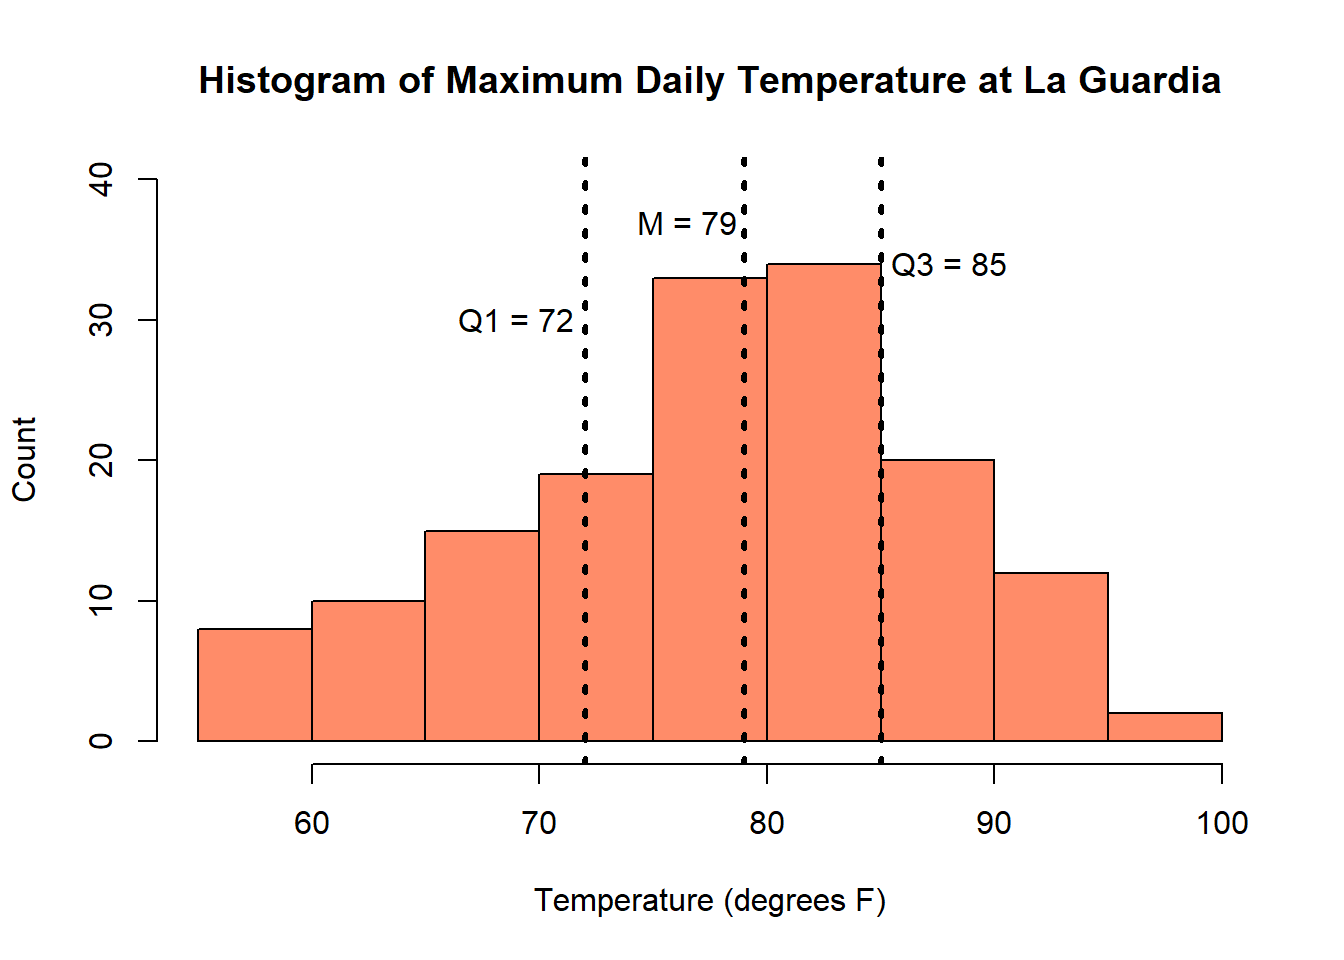
\includegraphics{introTextbookTemplate_files/figure-latex/unnamed-chunk-18-1.pdf}

Here is a as.raw(c(0x25, 0x50, 0x44, 0x46, 0x2d, 0x31, 0x2e, 0x34, 0x0a, 0x25, 0xc3, 0xa2, 0xc3, 0xa3, 0x0a, 0x31, 0x20, 0x30, 0x20, 0x6f, 0x62, 0x6a, 0x0a, 0x3c, 0x3c, 0x0a, 0x2f, 0x54, 0x69, 0x74, 0x6c, 0x65, 0x20, 0x28, 0x29, 0x0a, 0x2f, 0x43, 0x72, 0x65, 0x61, 0x74, 0x6f, 0x72, 0x20, 0x28, 0x29, 0x0a, 0x2f, 0x50, 0x72, 0x6f, 0x64, 0x75, 0x63, 0x65, 0x72, 0x20, 0x28, 0xfe, 0xff, 0x00, 0x51, 0x00, 0x74, 0x00, 0x20, 0x00, 0x35, 0x00, 0x2e, 0x00, 0x31, 0x00, 0x32, 0x00, 0x2e, 0x00, 0x38, 0x29, 0x0a, 0x2f,
0x43, 0x72, 0x65, 0x61, 0x74, 0x69, 0x6f, 0x6e, 0x44, 0x61, 0x74, 0x65, 0x20, 0x28, 0x44, 0x3a, 0x32, 0x30, 0x32, 0x31, 0x30, 0x36, 0x32, 0x31, 0x31, 0x30, 0x32, 0x31, 0x30, 0x33, 0x2d, 0x30, 0x35, 0x27, 0x30, 0x30, 0x27, 0x29, 0x0a, 0x3e, 0x3e, 0x0a, 0x65, 0x6e, 0x64, 0x6f, 0x62, 0x6a, 0x0a, 0x32, 0x20, 0x30, 0x20, 0x6f, 0x62, 0x6a, 0x0a, 0x3c, 0x3c, 0x0a, 0x2f, 0x54, 0x79, 0x70, 0x65, 0x20, 0x2f, 0x43, 0x61, 0x74, 0x61, 0x6c, 0x6f, 0x67, 0x0a, 0x2f, 0x50, 0x61, 0x67, 0x65, 0x73, 0x20, 0x33, 0x20,
0x30, 0x20, 0x52, 0x0a, 0x3e, 0x3e, 0x0a, 0x65, 0x6e, 0x64, 0x6f, 0x62, 0x6a, 0x0a, 0x34, 0x20, 0x30, 0x20, 0x6f, 0x62, 0x6a, 0x0a, 0x3c, 0x3c, 0x0a, 0x2f, 0x54, 0x79, 0x70, 0x65, 0x20, 0x2f, 0x45, 0x78, 0x74, 0x47, 0x53, 0x74, 0x61, 0x74, 0x65, 0x0a, 0x2f, 0x53, 0x41, 0x20, 0x74, 0x72, 0x75, 0x65, 0x0a, 0x2f, 0x53, 0x4d, 0x20, 0x30, 0x2e, 0x30, 0x32, 0x0a, 0x2f, 0x63, 0x61, 0x20, 0x31, 0x2e, 0x30, 0x0a, 0x2f, 0x43, 0x41, 0x20, 0x31, 0x2e, 0x30, 0x0a, 0x2f, 0x41, 0x49, 0x53, 0x20, 0x66, 0x61, 0x6c,
0x73, 0x65, 0x0a, 0x2f, 0x53, 0x4d, 0x61, 0x73, 0x6b, 0x20, 0x2f, 0x4e, 0x6f, 0x6e, 0x65, 0x3e, 0x3e, 0x0a, 0x65, 0x6e, 0x64, 0x6f, 0x62, 0x6a, 0x0a, 0x35, 0x20, 0x30, 0x20, 0x6f, 0x62, 0x6a, 0x0a, 0x5b, 0x2f, 0x50, 0x61, 0x74, 0x74, 0x65, 0x72, 0x6e, 0x20, 0x2f, 0x44, 0x65, 0x76, 0x69, 0x63, 0x65, 0x52, 0x47, 0x42, 0x5d, 0x0a, 0x65, 0x6e, 0x64, 0x6f, 0x62, 0x6a, 0x0a, 0x36, 0x20, 0x30, 0x20, 0x6f, 0x62, 0x6a, 0x0a, 0x3c, 0x3c, 0x0a, 0x2f, 0x54, 0x79, 0x70, 0x65, 0x20, 0x2f, 0x50, 0x61, 0x67, 0x65,
0x0a, 0x2f, 0x50, 0x61, 0x72, 0x65, 0x6e, 0x74, 0x20, 0x33, 0x20, 0x30, 0x20, 0x52, 0x0a, 0x2f, 0x43, 0x6f, 0x6e, 0x74, 0x65, 0x6e, 0x74, 0x73, 0x20, 0x37, 0x20, 0x30, 0x20, 0x52, 0x0a, 0x2f, 0x52, 0x65, 0x73, 0x6f, 0x75, 0x72, 0x63, 0x65, 0x73, 0x20, 0x39, 0x20, 0x30, 0x20, 0x52, 0x0a, 0x2f, 0x41, 0x6e, 0x6e, 0x6f, 0x74, 0x73, 0x20, 0x31, 0x30, 0x20, 0x30, 0x20, 0x52, 0x0a, 0x2f, 0x4d, 0x65, 0x64, 0x69, 0x61, 0x42, 0x6f, 0x78, 0x20, 0x5b, 0x30, 0x20, 0x30, 0x20, 0x34, 0x36, 0x38, 0x2e, 0x30, 0x30,
0x30, 0x30, 0x30, 0x30, 0x20, 0x33, 0x32, 0x34, 0x2e, 0x30, 0x30, 0x30, 0x30, 0x30, 0x30, 0x5d, 0x0a, 0x3e, 0x3e, 0x0a, 0x65, 0x6e, 0x64, 0x6f, 0x62, 0x6a, 0x0a, 0x39, 0x20, 0x30, 0x20, 0x6f, 0x62, 0x6a, 0x0a, 0x3c, 0x3c, 0x0a, 0x2f, 0x43, 0x6f, 0x6c, 0x6f, 0x72, 0x53, 0x70, 0x61, 0x63, 0x65, 0x20, 0x3c, 0x3c, 0x0a, 0x2f, 0x50, 0x43, 0x53, 0x70, 0x20, 0x35, 0x20, 0x30, 0x20, 0x52, 0x0a, 0x2f, 0x43, 0x53, 0x70, 0x20, 0x2f, 0x44, 0x65, 0x76, 0x69, 0x63, 0x65, 0x52, 0x47, 0x42, 0x0a, 0x2f, 0x43, 0x53,
0x70, 0x67, 0x20, 0x2f, 0x44, 0x65, 0x76, 0x69, 0x63, 0x65, 0x47, 0x72, 0x61, 0x79, 0x0a, 0x3e, 0x3e, 0x0a, 0x2f, 0x45, 0x78, 0x74, 0x47, 0x53, 0x74, 0x61, 0x74, 0x65, 0x20, 0x3c, 0x3c, 0x0a, 0x2f, 0x47, 0x53, 0x61, 0x20, 0x34, 0x20, 0x30, 0x20, 0x52, 0x0a, 0x3e, 0x3e, 0x0a, 0x2f, 0x50, 0x61, 0x74, 0x74, 0x65, 0x72, 0x6e, 0x20, 0x3c, 0x3c, 0x0a, 0x3e, 0x3e, 0x0a, 0x2f, 0x46, 0x6f, 0x6e, 0x74, 0x20, 0x3c, 0x3c, 0x0a, 0x3e, 0x3e, 0x0a, 0x2f, 0x58, 0x4f, 0x62, 0x6a, 0x65, 0x63, 0x74, 0x20, 0x3c, 0x3c,
0x0a, 0x3e, 0x3e, 0x0a, 0x3e, 0x3e, 0x0a, 0x65, 0x6e, 0x64, 0x6f, 0x62, 0x6a, 0x0a, 0x31, 0x30, 0x20, 0x30, 0x20, 0x6f, 0x62, 0x6a, 0x0a, 0x5b, 0x20, 0x5d, 0x0a, 0x65, 0x6e, 0x64, 0x6f, 0x62, 0x6a, 0x0a, 0x37, 0x20, 0x30, 0x20, 0x6f, 0x62, 0x6a, 0x0a, 0x3c, 0x3c, 0x0a, 0x2f, 0x4c, 0x65, 0x6e, 0x67, 0x74, 0x68, 0x20, 0x38, 0x20, 0x30, 0x20, 0x52, 0x0a, 0x2f, 0x46, 0x69, 0x6c, 0x74, 0x65, 0x72, 0x20, 0x2f, 0x46, 0x6c, 0x61, 0x74, 0x65, 0x44, 0x65, 0x63, 0x6f, 0x64, 0x65, 0x0a, 0x3e, 0x3e, 0x0a, 0x73,
0x74, 0x72, 0x65, 0x61, 0x6d, 0x0a, 0x78, 0x9c, 0xd3, 0x77, 0x0f, 0x4e, 0x54, 0x48, 0x2f, 0x56, 0xd0, 0x77, 0x0e, 0x2e, 0x50, 0x48, 0x86, 0xd2, 0xce, 0xc1, 0x5c, 0x86, 0x0a, 0x06, 0x40, 0xa8, 0x0b, 0xa2, 0x8c, 0x8d, 0x4c, 0x14, 0x92, 0x73, 0xb9, 0x0a, 0x15, 0x0a, 0xb9, 0x02, 0xb9, 0x02, 0x81, 0x24, 0x88, 0x2e, 0xe4, 0x32, 0xd0, 0x33, 0x37, 0x35, 0x80, 0x00, 0xb0, 0x5a, 0x74, 0x3e, 0x50, 0x0b, 0xcc, 0x50, 0x88, 0x40, 0x71, 0x72, 0x1e, 0x97, 0x3e, 0xc4, 0x3a, 0x2e, 0x88, 0x48, 0xb0, 0xb3, 0x1f, 0xd0,
0xa2, 0x72, 0x20, 0xcb, 0x4b, 0xc1, 0x48, 0xc1, 0x17, 0x48, 0x67, 0x29, 0x44, 0xc7, 0x1a, 0x28, 0x28, 0xa4, 0x40, 0x6d, 0x02, 0x29, 0xca, 0xe5, 0x32, 0x31, 0xb3, 0xd0, 0x03, 0x9b, 0x6b, 0x06, 0xe4, 0xe6, 0x20, 0x73, 0x81, 0x4e, 0x83, 0x30, 0x4d, 0x80, 0xe2, 0x06, 0xe8, 0x5c, 0x90, 0xe2, 0x0c, 0xae, 0x70, 0x2d, 0x85, 0x3c, 0xb0, 0x73, 0xcd, 0xa0, 0xae, 0xb3, 0x80, 0x3a, 0x17, 0x95, 0x4f, 0x0d, 0xe7, 0xd2, 0x3c, 0x50, 0x14, 0x02, 0xb9, 0x00, 0x3f, 0x1c, 0x5b, 0xa7, 0x0a, 0x65, 0x6e, 0x64, 0x73, 0x74,
0x72, 0x65, 0x61, 0x6d, 0x0a, 0x65, 0x6e, 0x64, 0x6f, 0x62, 0x6a, 0x0a, 0x38, 0x20, 0x30, 0x20, 0x6f, 0x62, 0x6a, 0x0a, 0x31, 0x35, 0x36, 0x0a, 0x65, 0x6e, 0x64, 0x6f, 0x62, 0x6a, 0x0a, 0x33, 0x20, 0x30, 0x20, 0x6f, 0x62, 0x6a, 0x0a, 0x3c, 0x3c, 0x0a, 0x2f, 0x54, 0x79, 0x70, 0x65, 0x20, 0x2f, 0x50, 0x61, 0x67, 0x65, 0x73, 0x0a, 0x2f, 0x4b, 0x69, 0x64, 0x73, 0x20, 0x0a, 0x5b, 0x0a, 0x36, 0x20, 0x30, 0x20, 0x52, 0x0a, 0x5d, 0x0a, 0x2f, 0x43, 0x6f, 0x75, 0x6e, 0x74, 0x20, 0x31, 0x0a, 0x2f, 0x50, 0x72,
0x6f, 0x63, 0x53, 0x65, 0x74, 0x20, 0x5b, 0x2f, 0x50, 0x44, 0x46, 0x20, 0x2f, 0x54, 0x65, 0x78, 0x74, 0x20, 0x2f, 0x49, 0x6d, 0x61, 0x67, 0x65, 0x42, 0x20, 0x2f, 0x49, 0x6d, 0x61, 0x67, 0x65, 0x43, 0x5d, 0x0a, 0x3e, 0x3e, 0x0a, 0x65, 0x6e, 0x64, 0x6f, 0x62, 0x6a, 0x0a, 0x78, 0x72, 0x65, 0x66, 0x0a, 0x30, 0x20, 0x31, 0x31, 0x0a, 0x30, 0x30, 0x30, 0x30, 0x30, 0x30, 0x30, 0x30, 0x30, 0x30, 0x20, 0x36, 0x35, 0x35, 0x33, 0x35, 0x20, 0x66, 0x20, 0x0a, 0x30, 0x30, 0x30, 0x30, 0x30, 0x30, 0x30, 0x30, 0x31,
0x35, 0x20, 0x30, 0x30, 0x30, 0x30, 0x30, 0x20, 0x6e, 0x20, 0x0a, 0x30, 0x30, 0x30, 0x30, 0x30, 0x30, 0x30, 0x31, 0x33, 0x31, 0x20, 0x30, 0x30, 0x30, 0x30, 0x30, 0x20, 0x6e, 0x20, 0x0a, 0x30, 0x30, 0x30, 0x30, 0x30, 0x30, 0x30, 0x38, 0x36, 0x39, 0x20, 0x30, 0x30, 0x30, 0x30, 0x30, 0x20, 0x6e, 0x20, 0x0a, 0x30, 0x30, 0x30, 0x30, 0x30, 0x30, 0x30, 0x31, 0x38, 0x30, 0x20, 0x30, 0x30, 0x30, 0x30, 0x30, 0x20, 0x6e, 0x20, 0x0a, 0x30, 0x30, 0x30, 0x30, 0x30, 0x30, 0x30, 0x32, 0x37, 0x35, 0x20, 0x30, 0x30,
0x30, 0x30, 0x30, 0x20, 0x6e, 0x20, 0x0a, 0x30, 0x30, 0x30, 0x30, 0x30, 0x30, 0x30, 0x33, 0x31, 0x32, 0x20, 0x30, 0x30, 0x30, 0x30, 0x30, 0x20, 0x6e, 0x20, 0x0a, 0x30, 0x30, 0x30, 0x30, 0x30, 0x30, 0x30, 0x36, 0x32, 0x30, 0x20, 0x30, 0x30, 0x30, 0x30, 0x30, 0x20, 0x6e, 0x20, 0x0a, 0x30, 0x30, 0x30, 0x30, 0x30, 0x30, 0x30, 0x38, 0x35, 0x30, 0x20, 0x30, 0x30, 0x30, 0x30, 0x30, 0x20, 0x6e, 0x20, 0x0a, 0x30, 0x30, 0x30, 0x30, 0x30, 0x30, 0x30, 0x34, 0x34, 0x35, 0x20, 0x30, 0x30, 0x30, 0x30, 0x30, 0x20,
0x6e, 0x20, 0x0a, 0x30, 0x30, 0x30, 0x30, 0x30, 0x30, 0x30, 0x36, 0x30, 0x30, 0x20, 0x30, 0x30, 0x30, 0x30, 0x30, 0x20, 0x6e, 0x20, 0x0a, 0x74, 0x72, 0x61, 0x69, 0x6c, 0x65, 0x72, 0x0a, 0x3c, 0x3c, 0x0a, 0x2f, 0x53, 0x69, 0x7a, 0x65, 0x20, 0x31, 0x31, 0x20, 0x0a, 0x2f, 0x49, 0x6e, 0x66, 0x6f, 0x20, 0x31, 0x20, 0x30, 0x20, 0x52, 0x0a, 0x2f, 0x52, 0x6f, 0x6f, 0x74, 0x20, 0x32, 0x20, 0x30, 0x20, 0x52, 0x0a, 0x3e, 0x3e, 0x0a, 0x73, 0x74, 0x61, 0x72, 0x74, 0x78, 0x72, 0x65, 0x66, 0x0a, 0x39, 0x36, 0x37,
0x20, 0x0a, 0x25, 0x25, 0x45, 0x4f, 0x46, 0x0a)), .pdf, NULL

\hypertarget{ch4}{%
\chapter{Probability}\label{ch4}}

\begin{quote}
``The most important questions of life are, for the most part, really only problems of probability.'' - Pierre Simon, Marquis de Laplace
\end{quote}

Learning objectives

\begin{enumerate}
\def\labelenumi{\arabic{enumi}.}
\tightlist
\item
  Learn the scientific definition of probability
\item
  Conceptual understanding of randomness
\item
  Understand probability notation and operations
\item
  Learn about conditional probability
\item
  Use probabilities to calculate quantities of interest in diagnostic testing
\end{enumerate}

\hypertarget{ch4_s1}{%
\section{Understanding Randomness}\label{ch4_s1}}

If statistics is the science of uncertainty, then probability is the mechanism that allows us to quantify our uncertainty. People talk loosely about probability all the time. For example, what's the chance of rain tomorrow?" or ``how likely is it that drug A is better than drug B?'' However, for scientific purposes, we need to be more specific in terms of defining and using probabilities.

First let's introduce some definitions to help us talk about randomness and probability. First, a \textbf{random process} is any act or process that results in an outcome that cannot be predicted with certainty. The \textbf{sample space} of a random process is the set of all its possible outcomes and is often denoted \(\mathcal{S}\). Finally, an \textbf{event} is an outcome or collection of outcomes from a random process and will always be contained in the sample space.

To illustrate, suppose we flip a fair coin three times. Each act of flipping the coin is random process - the coin might land on heads and it might land on tails. Letting \(H\) be shorthand for the flip resulting in heads and \(T\) be shorthand for the flip resulting in tails, the sample space can be enumerated as

\[\mathcal{S} = \{HHH, HHT, HTH, THH, TTH, THT, HTT, TTT\},\]

giving us eight possible results from the three coin flips. Finally, an event could be any single outcome, or any collection of outcomes, based on this experiment. For example, we may have:

\begin{itemize}
\tightlist
\item
  The event of obtaining \emph{exactly} two heads: \(\{HHT, HTH, THH\}\)\\
\item
  The event of obtaining heads on the first toss: \(\{HHH, HHT, HTH, HTT\}\)\\
\item
  The event of obtaining three tails \(\{TTT\}\).
\end{itemize}

We would all agree that the probability of heads when flipping a fair coin is 50\% and the probability of rolling a 2 on a 6-sided die is 1/6, but why is that true? Well, if we were to flip a coin many, many times, we would expect half of the flips to result in heads. Similarly, if we roll a 6-sided die over and over, 1/6 of the rolls should result in a value of 2. In both cases, we are thinking about a long-run frequency, which is why \textbf{probability} is defined as the fraction of time an event occurs if a random process is repeated over and over again under the same conditions. This means that probabilities are always between 0 and 1, since we can never observed more events than the number of times the process is repeated, e.g.~we can never observed 12 heads on 10 coin flips. \sout{Clearly, an event with probability 0 is an event that can never occur.}

This leads us to some important properties of probabilities:

\begin{enumerate}
\def\labelenumi{\arabic{enumi})}
\tightlist
\item
  The sum of probabilities for all outcomes in the sample space, \(\mathcal{S}\), must equal 1
\item
  For any event, the probability of that event is the sum of the probabilities for all the outcomes in that event
\end{enumerate}

For the coin flipping example, there are eight possible outcomes. Since each outcome is equally likely (why?) The first property tells us that the probability of any specific outcome (say, \(HHH\)) is 1/8. The second tells us that the probability of heads on the first toss is \(4/8 = 1/2\), since four of the outcomes. These properties underlie a lot of the more complicated formulas and concepts we will cover in this chapter, although we don't always think about them explicitly.

We can explore this concept of long-run frequency more with a simulation. For this simulation, we will simulate rolling a 6-sided die 100 times, recording the result of each roll, and then tabulating the proportion of rolls where we observed each side of the die.

\begin{Shaded}
\begin{Highlighting}[]
\NormalTok{rollDie }\OtherTok{\textless{}{-}} \ControlFlowTok{function}\NormalTok{(nRolls, seed) \{}
    \FunctionTok{set.seed}\NormalTok{(seed)}
    \FunctionTok{sample}\NormalTok{(}\DecValTok{1}\SpecialCharTok{:}\DecValTok{6}\NormalTok{, nRolls, }\AttributeTok{replace =} \ConstantTok{TRUE}\NormalTok{)}
\NormalTok{\}}
\FunctionTok{barplot}\NormalTok{(}\FunctionTok{table}\NormalTok{(}\FunctionTok{rollDie}\NormalTok{(}\DecValTok{100}\NormalTok{, }\DecValTok{1}\NormalTok{)))}
\end{Highlighting}
\end{Shaded}

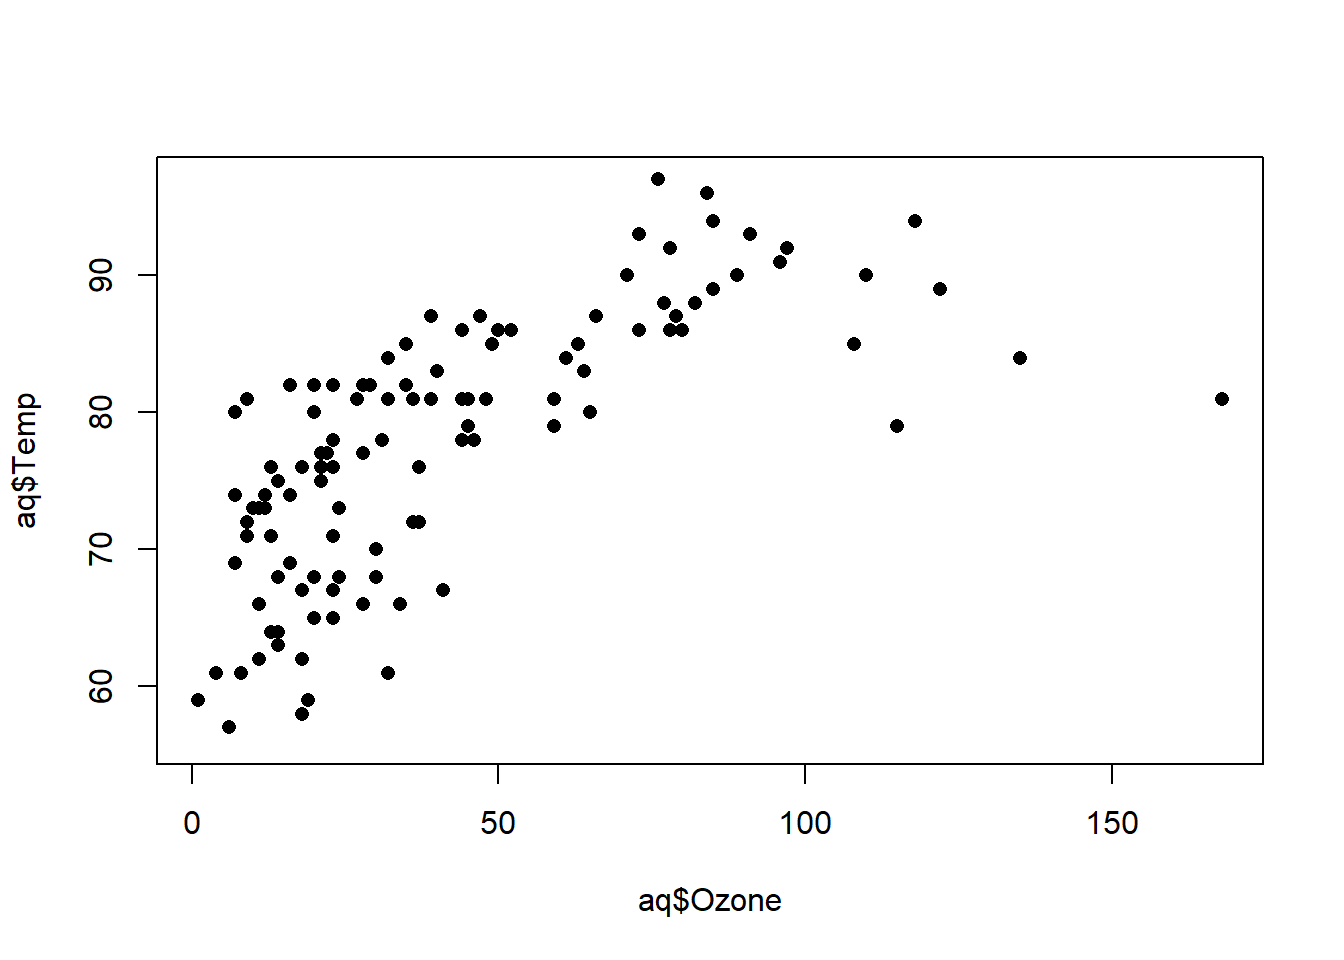
\includegraphics{introTextbookTemplate_files/figure-latex/unnamed-chunk-19-1.pdf}

\begin{Shaded}
\begin{Highlighting}[]
\FunctionTok{prop.table}\NormalTok{(}\FunctionTok{table}\NormalTok{(}\FunctionTok{rollDie}\NormalTok{(}\DecValTok{100}\NormalTok{, }\DecValTok{1}\NormalTok{)))}
\end{Highlighting}
\end{Shaded}

\begin{verbatim}
## 
##    1    2    3    4    5    6 
## 0.19 0.18 0.12 0.15 0.15 0.21
\end{verbatim}

As we see, with just 100 rolls, we don't observe exactly the same proportion of rolls landing on each side of the die. The proportions are not exactly 1/6 = 16.7\%, because of randomness. However, if we do 1,000,000 rolls, we see things even out:

\begin{Shaded}
\begin{Highlighting}[]
\FunctionTok{round}\NormalTok{(}\FunctionTok{prop.table}\NormalTok{(}\FunctionTok{table}\NormalTok{(}\FunctionTok{rollDie}\NormalTok{(}\FloatTok{1e6}\NormalTok{, }\DecValTok{1}\NormalTok{))), }\DecValTok{3}\NormalTok{)}
\end{Highlighting}
\end{Shaded}

\begin{verbatim}
## 
##     1     2     3     4     5     6 
## 0.167 0.167 0.167 0.167 0.167 0.166
\end{verbatim}

Now let users play with a similar app illustrating coin flips (or something) and have associated exercises. Maybe a plot of the proportion over time.

\hypertarget{ch4_s2}{%
\section{Probability Operations}\label{ch4_s2}}

It's easy to talk about probability of one event, i.e.~the probability of rolling a 2, but often we are interested in quantifying probabilities about more complicated combinations of multiple events. For example, if we consider a family with two parents and one child, instead of the probability of one parent getting the flu, we might be interested in the probability that \emph{both} parents get the flu. Or we might be interested in the probability \emph{anyone} in the family gets the flu. Finally, we might want to quantify the probability that one parent gets the flu and the other does not. In order to succinctly describe these probabilities, we use some mathematical notation. Before you get totally scared, this notation is just to simplify the writing of probability statements - the underlying concept does not change!

Probabilities are denoted as \(P(Event) = p\), as in \(P(Heads) = 0.5\). To make things even shorter we can use a capital letter to denote an event of interest, i.e.~let \(H\) be the event that the outcome of a fair coin flip is heads, then we have \(P(H) = 0.5\). Then, to talk about relationships between events, we define the operations of the \textbf{intersection}, \textbf{union}, and \textbf{complement}. Consider to arbitrary events \(A\) and \(B\):

\begin{itemize}
\tightlist
\item
  The intersection represents the event that \(A\) and \(B\) occur and is denoted \(A \cap B\)\\
\item
  The union represents the event that \(A\) or \(B\) occur and is denoted \(A \cup B\)\\
\item
  The complement represents the scenario in which an event does not occur; the complement of \(A\) is denoted as \(A^C\). As a corollary to this, for any event \(A\), we could say that \(A\) occurs or \(A\) does not occur \((A^C)\). As these are the only possible outcomes regarding \(A\), \(A \cup A^C\) represents all possible events, or \(A \cup A^C = \mathcal{S}\)
\end{itemize}

In the previous coin tossing example, define \(A = \text{obtaining exactly two heads} = \{HHT, HTH, THH\}\) and \(B = \text{obtaining heads on the first toss} = \{HHH, HHT, HTH, HTT\}\).

\begin{itemize}
\tightlist
\item
  \(A \cap B = \text{obtaining exactly two heads AND a heads on the first toss} = \{HHT, HTH\}\)
\item
  \(A \cup B = \text{obtaining exactly two heads OR a heads on the first toss}= \{HHH, HHT, HTH, HTT, THH\}\)
\item
  \(B^C = \text{obtaining tails on the first toss} = \{TTH, THT, THH, TTT\}\)
\end{itemize}

We can visualize these operations with Venn diagrams. A Venn diagram uses overlapping circles and shading to describe the relationship between two events. First, we will visualize the intersection operation. If the left circle denotes the event \(A\) and the right circle denotes the event \(B\), then the intersection is the overlapping region where both \(A\) and \(B\) occur.

\begin{figure}

{\centering 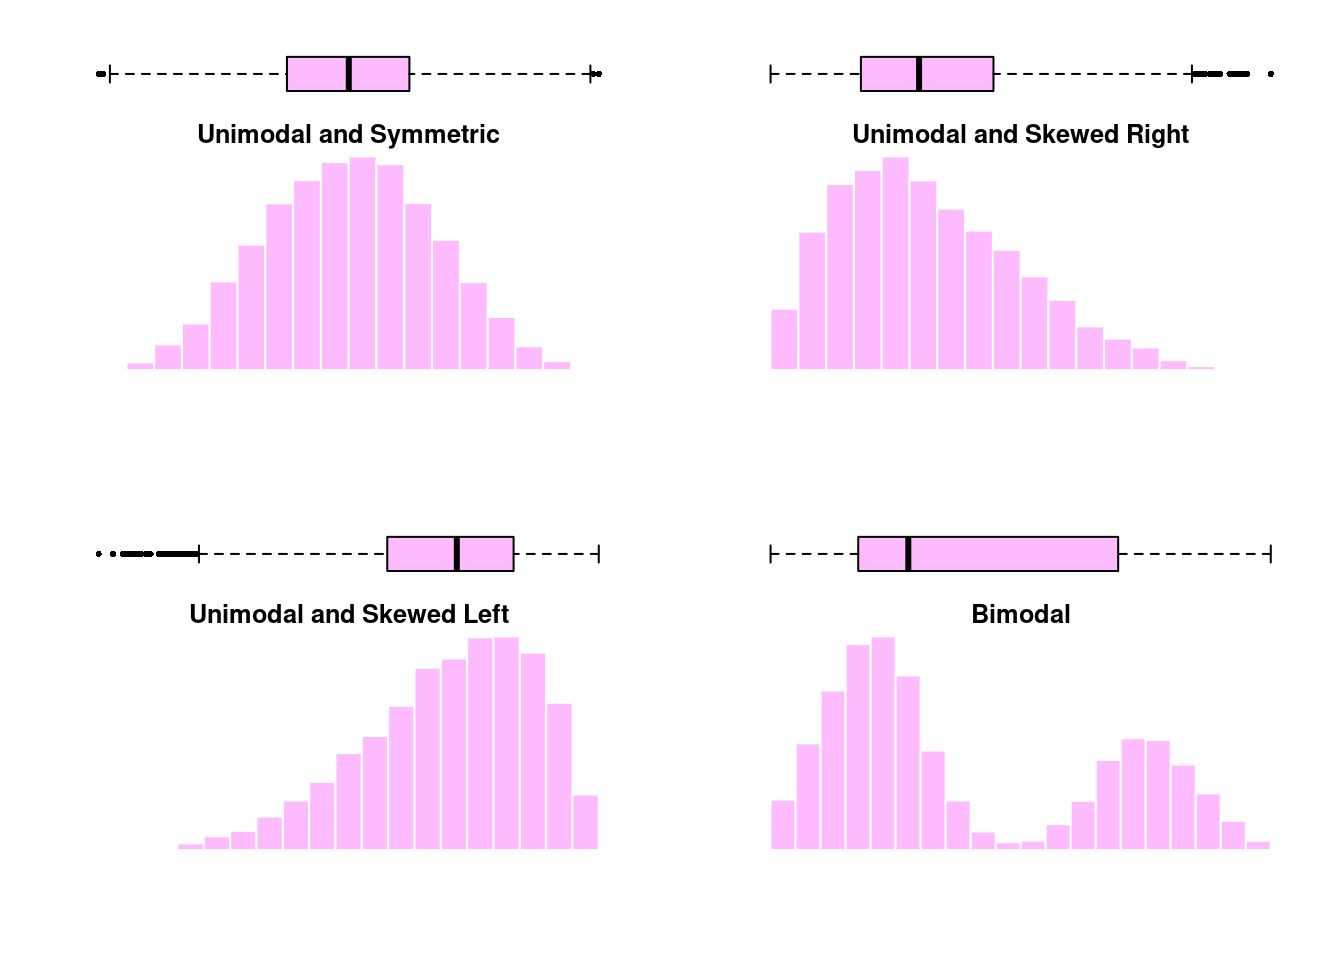
\includegraphics{introTextbookTemplate_files/figure-latex/unnamed-chunk-21-1} 

}

\caption{Venn diagram of intersection}\label{fig:unnamed-chunk-21}
\end{figure}

The union operation includes all outcomes in \(A\) or \(B\) (or both), so it would include the entire region.

\begin{figure}

{\centering 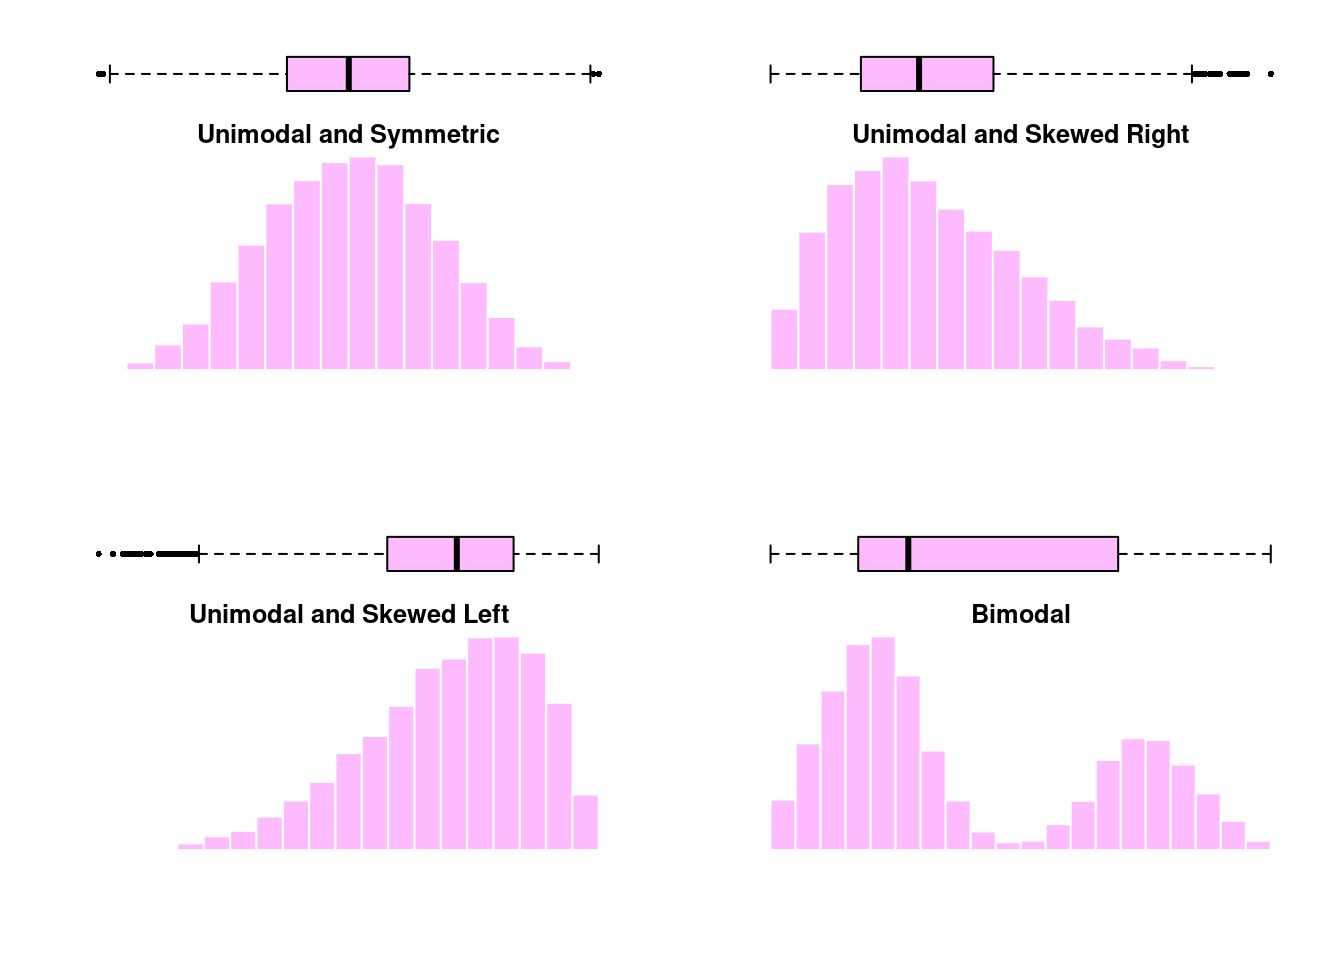
\includegraphics{introTextbookTemplate_files/figure-latex/unnamed-chunk-22-1} 

}

\caption{Venn diagram of union}\label{fig:unnamed-chunk-22}
\end{figure}

The complement of \(B\), includes all outcomes that are \emph{not} part of event \(B\).

\begin{figure}

{\centering 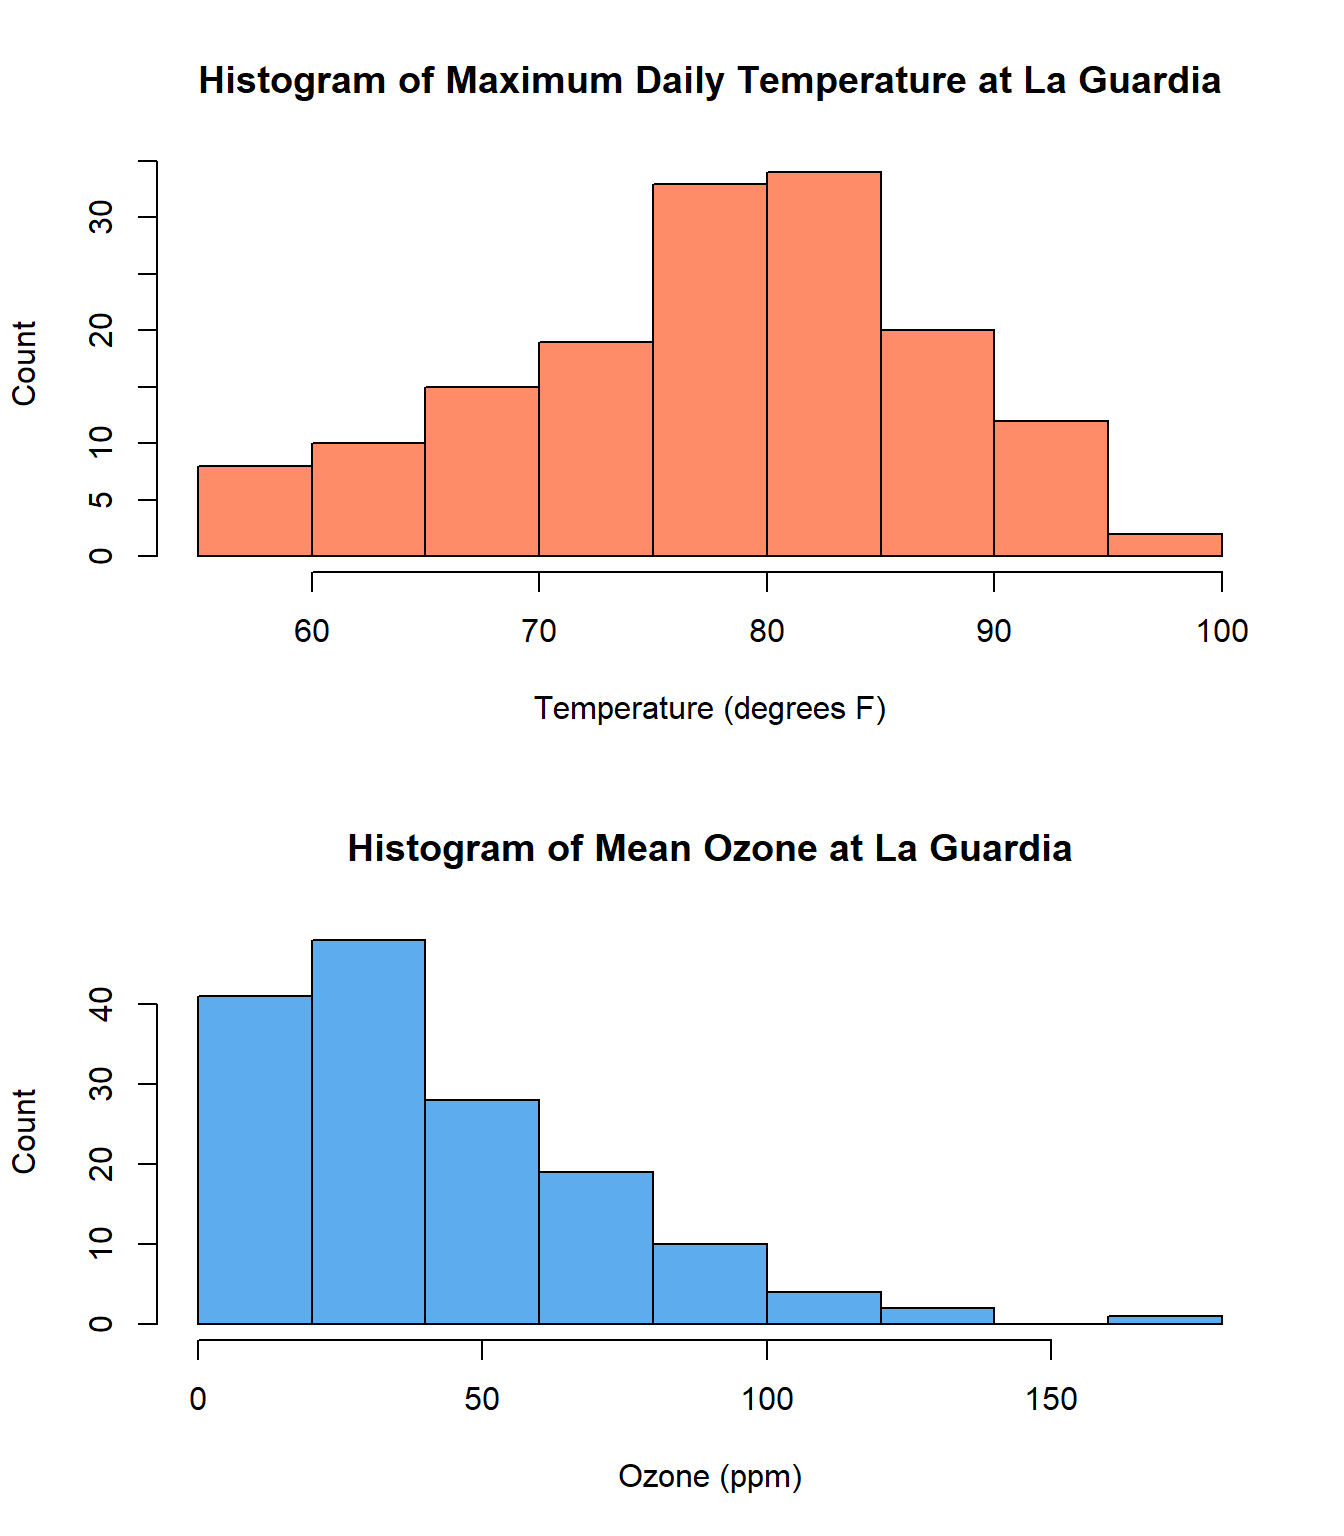
\includegraphics{introTextbookTemplate_files/figure-latex/unnamed-chunk-23-1} 

}

\caption{Venn diagram of the complement of B}\label{fig:unnamed-chunk-23}
\end{figure}

Since the probability of all outcomes in the sample space must add to 1, and the complement

Back to the flu example, let \(A\) denote the event that one parent gets the flu, let \(B\) denote the event that the other parent gets the flu, and let \(C\) denote the event that the child gets the flu. Using this new notation, we can represent the probability that both parents get the flu as \(P(A \cap B)\) , the probability that anyone in the family gets the flu as \(P(A \cup B \cup C)\), and the probability that one parent gets the flu and the other does not as \(P(A \cap B^C)\).

In some cases, there is no overlap between the events, i.e.~the events cannot happen simultaneously. When two events cannot happen at the same time, they are said to be \textbf{mutually exclusive}. Mathematically, this means the \(P(A \cap B) = 0\). For example, consider the following two events based on your final course letter grade: \(A\) is the event of getting an \(A\) and \(B\) is the event of getting a \(B\). As only one grade can be given per course, clearly \(A\) and \(B\) are mutually exclusive. Obtaining the probability of at least one of two mutually exclusive events happening is straightforward as there is no overlap between events. Thus, the probability of \(A \cup B\) is simply the sum of the probabilities of \(A\) and \(B\) happening separately.

Important Formula!

For mutually exclusive events:
\[P(A \cup B) = P(A) + P(B)\]

\begin{figure}

{\centering 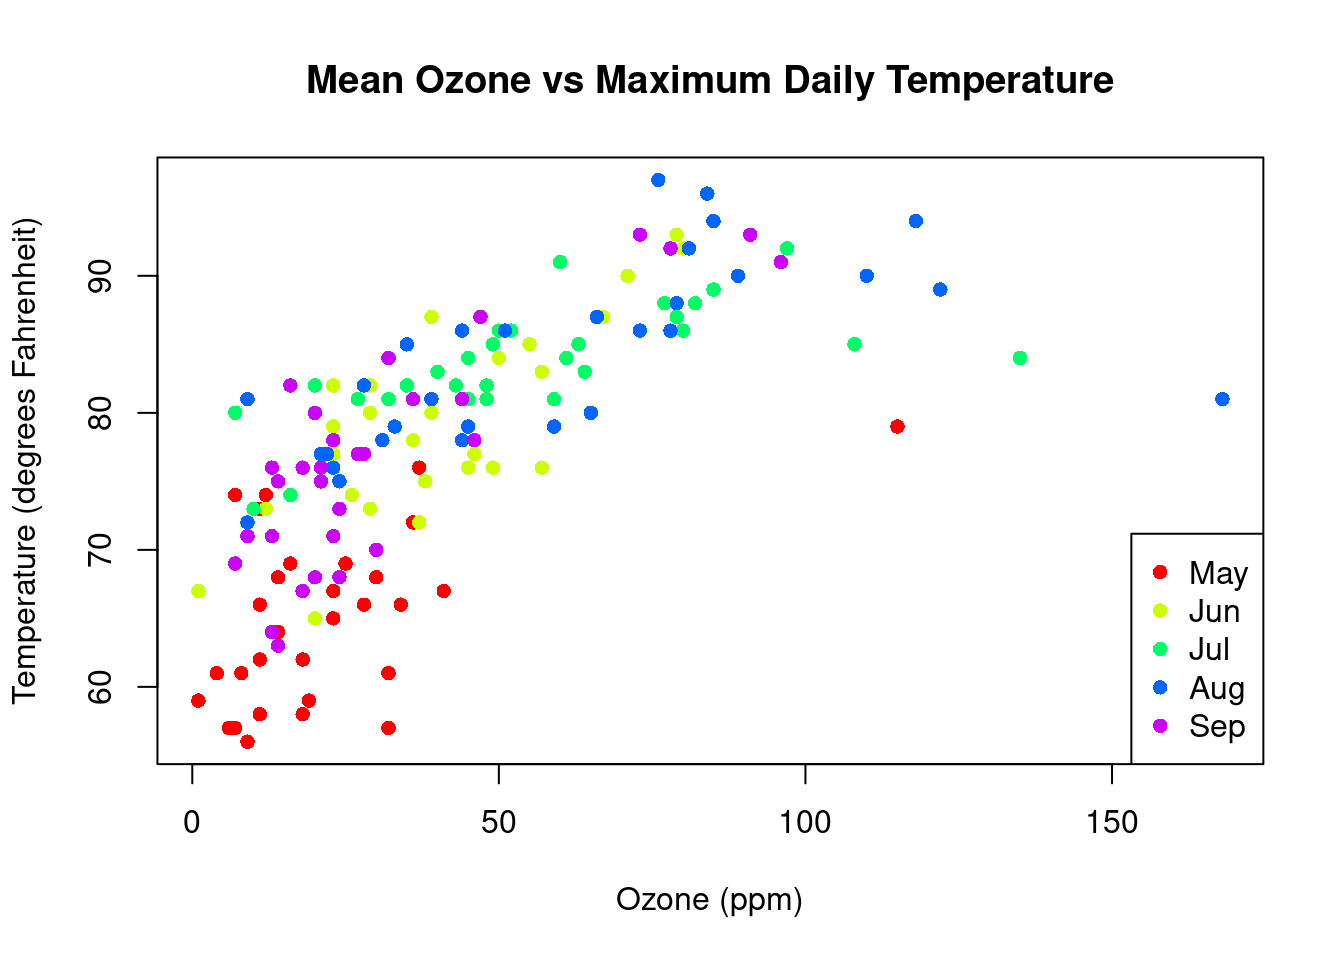
\includegraphics{introTextbookTemplate_files/figure-latex/unnamed-chunk-24-1} 

}

\caption{Venn diagram of mutually exclusive events}\label{fig:unnamed-chunk-24}
\end{figure}

If two events are not mutually exclusive, there is overlap in the events and \(P(A \cap B) \neq 0\) and we cannot get the probability of the union using the previous formula. If we did, we would be double counting the intersection. As a concrete illustration, suppose that for a married couple, the probability that one spouse contracts the flu (event \(A\)) is 0.25, the probability that the other spouse contracts the flu (event \(B\)) is 0.20, and the probability that both the spouses contract the flu (\(A\) and \(B\)) is 0.15. If we displayed this information in a Venn Diagram, we would have:

\begin{figure}

{\centering 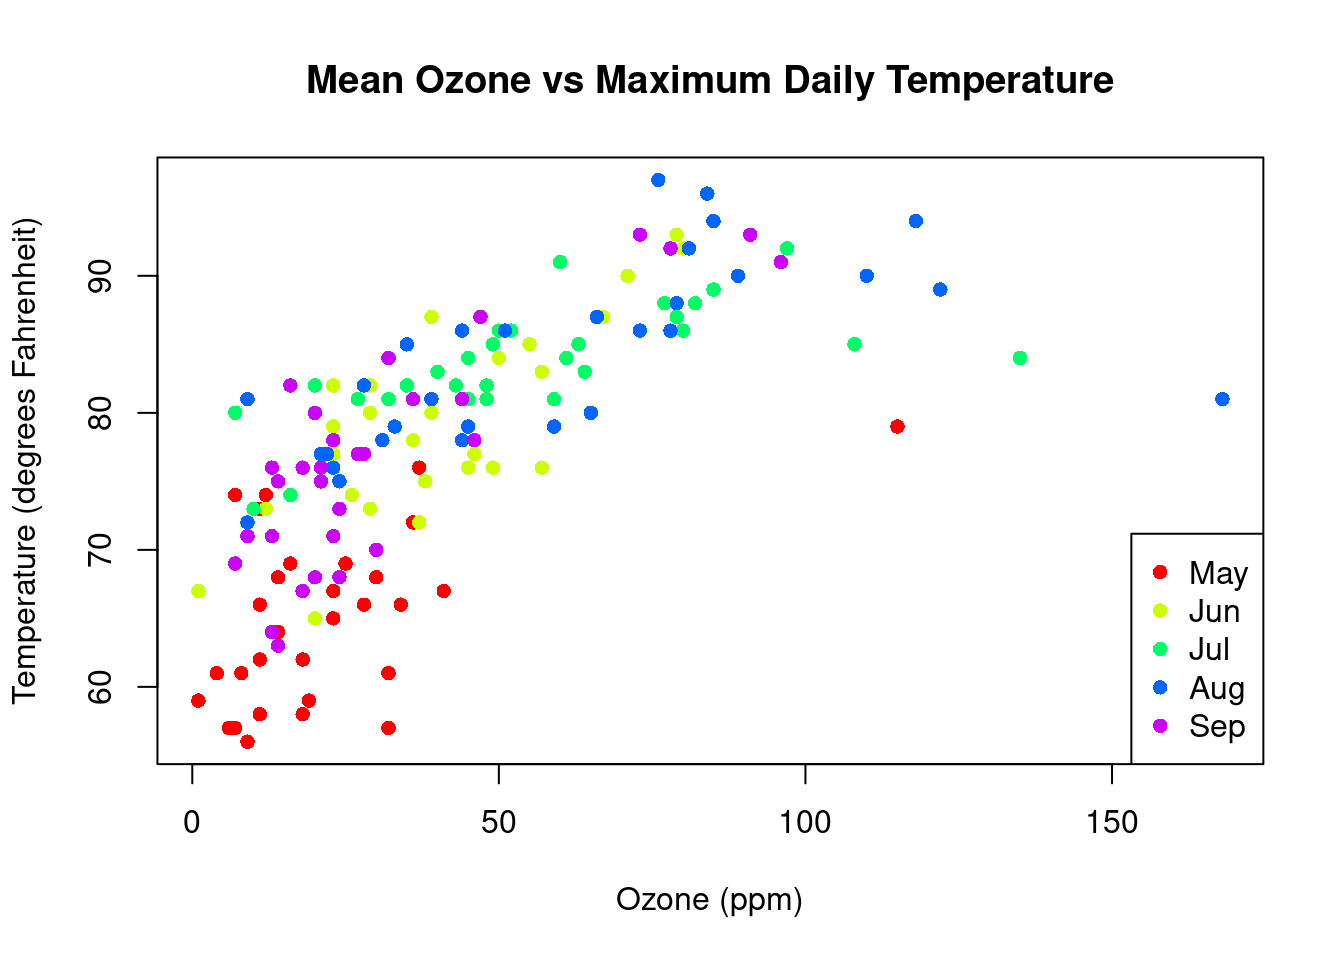
\includegraphics{introTextbookTemplate_files/figure-latex/unnamed-chunk-25-1} 

}

\caption{Venn diagram of flu probabilities}\label{fig:unnamed-chunk-25}
\end{figure}

At first glance, this might not be what you would expect. If \(P(A = 0.25)\), why do we have \(0.10\) in that region? However, the event \(A\) is actually divided into two regions - the part that intersects \(B\) and the part that doesn't. This is called the \textbf{Law of Total Probability}, and this means that the probability of \(A\) consists of both the probability that \(A\) and \(B\) both happen and the probability that \(A\) happens but \(B\) doesn't. This is true since \(B\) and \(B^C\) are mutually exclusive and together contain all possible outcomes. Mathematically, we can write this as:

\[P(A) = P(A \cap B) + P(A \cap B^C)\]

And in a Venn diagram this looks like:

\begin{figure}

{\centering 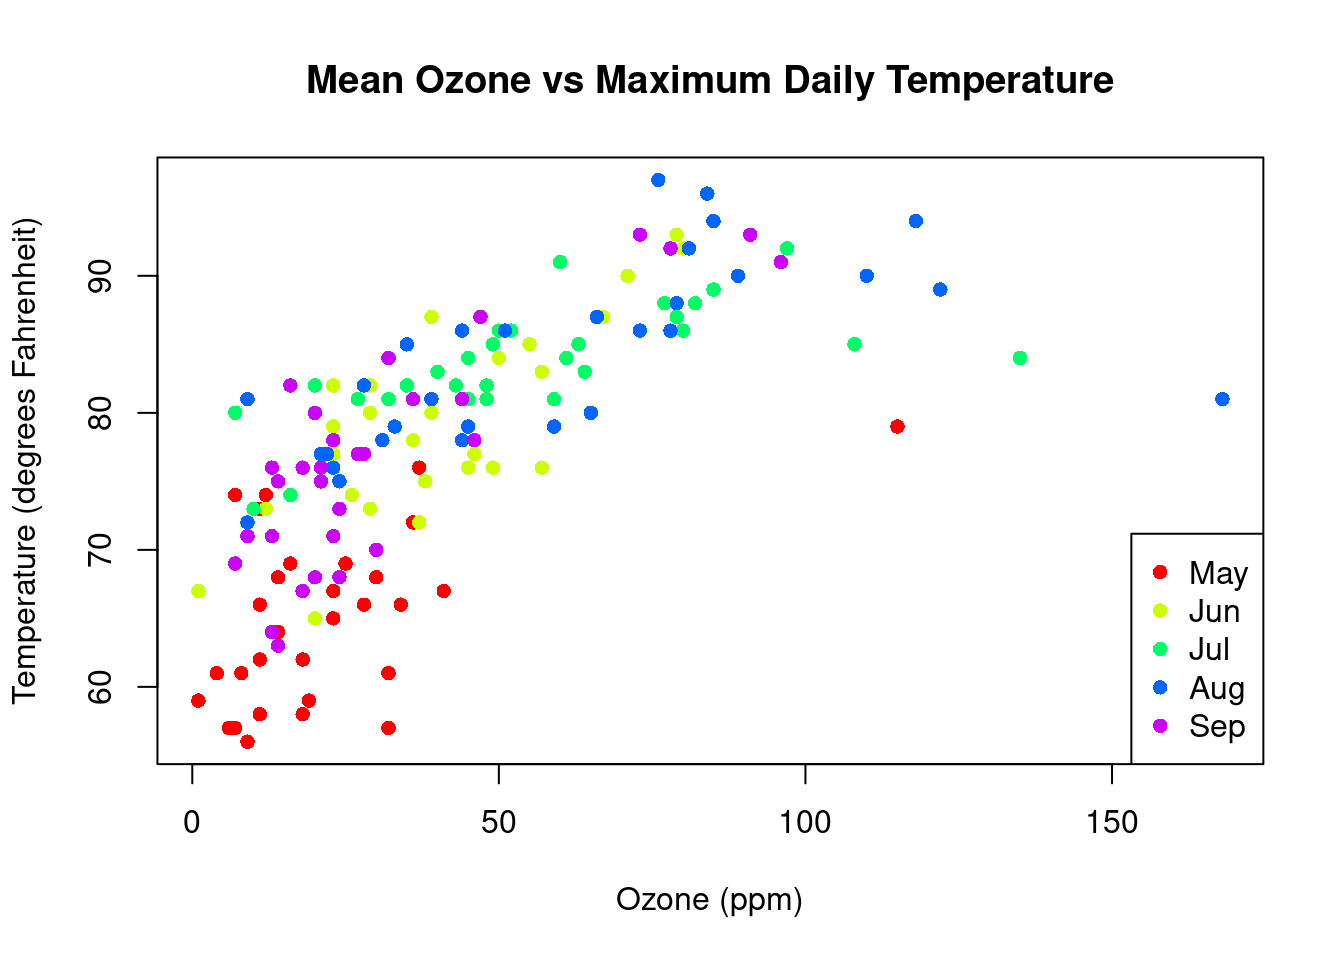
\includegraphics{introTextbookTemplate_files/figure-latex/unnamed-chunk-26-1} 

}

\caption{Venn diagram of the law of total probability}\label{fig:unnamed-chunk-26}
\end{figure}

Getting back to finding the quantity of interest, \(P(A \cup B)\), what all of this means is that if two events are not mutually exclusive, then \(P(A \cup B) \neq P(A) + P(B)\), because \emph{both} \(P(A)\) and \(P(B)\) include the intersection regions \(P(A \cap B)\). We do want to include the intersection in the union, but only one time. So we can get the correct probability by subtracting off \emph{one} of the intersections:

Important formula!!

In general,
\[P(A \cup B) = P(A) + P(B) - P(A \cap B)\]
This formula actually includes the mutually exclusive case, since when two events are mutually exclusive \(P(A \cap B) = 0\).

Let's use a coin flipping simulation to illustrate this formula with the two events of interest being obtaining exactly two heads (event \(A\)) and obtaining heads on the first toss (event \(B\)). We know there are three ways we can obtain exactly two heads, so \(P(A) = 3/8 = 0.375\). There are four ways we can obtain heads on the first toss, so \(P(B) = 4/8 = 0.50\). There are two ways we can obtain exactly two heads AND obtain heads on the first toss, so \(P(A \cap B) = 2/8 = 0.25\). Finally, there are five ways we can we can obtain exactly two heads OR obtain heads on the first toss, so \(P(A \cup B) = 5/8 = 0.625\). We could also find this last probability using the previous formula and the previous probabilities.

\[P(A \cup B) = P(A) + P(B) - P(A \cap B) = 0.375 = 0.50 - 0.25 = 0.625\]

You can decide how many simulations to run, and the app will report the proportion of simulations that results in exactly two heads, the proportion where heads was obtained on the first toss, the proportion were both events occurred simultaneously, and the proportion of where either event occurred. Since probabilities are defined as long run frequencies, if enough simulations are run, these proportions should be identical to the probabilities defined previously.

\begin{Shaded}
\begin{Highlighting}[]
\NormalTok{flipCoin3 }\OtherTok{\textless{}{-}} \ControlFlowTok{function}\NormalTok{() \{}
\NormalTok{    dat }\OtherTok{\textless{}{-}} \FunctionTok{rbinom}\NormalTok{(}\DecValTok{3}\NormalTok{, }\DecValTok{1}\NormalTok{, }\FloatTok{0.5}\NormalTok{)}
\NormalTok{    event1 }\OtherTok{\textless{}{-}} \FunctionTok{sum}\NormalTok{(dat) }\SpecialCharTok{==} \DecValTok{2}
\NormalTok{    event2 }\OtherTok{\textless{}{-}}\NormalTok{ dat[}\DecValTok{1}\NormalTok{] }\SpecialCharTok{==} \DecValTok{1}
\NormalTok{    intersectionProb }\OtherTok{\textless{}{-}}\NormalTok{ event1 }\SpecialCharTok{\&}\NormalTok{ event2}
\NormalTok{    unionProb }\OtherTok{\textless{}{-}}\NormalTok{ event1 }\SpecialCharTok{|}\NormalTok{ event2}
    
   \FunctionTok{c}\NormalTok{(event1, event2, intersectionProb, unionProb)}
\NormalTok{\}}

\NormalTok{nSims }\OtherTok{\textless{}{-}} \DecValTok{1000}

\NormalTok{simRes }\OtherTok{\textless{}{-}} \FunctionTok{replicate}\NormalTok{(nSims, }\FunctionTok{flipCoin3}\NormalTok{())}
\FunctionTok{cbind}\NormalTok{(}\FunctionTok{c}\NormalTok{(}\StringTok{\textquotesingle{}P(A)\textquotesingle{}}\NormalTok{, }\StringTok{\textquotesingle{}P(B)\textquotesingle{}}\NormalTok{, }\StringTok{\textquotesingle{}P(A AND B)\textquotesingle{}}\NormalTok{, }\StringTok{\textquotesingle{}P(A OR B)\textquotesingle{}}\NormalTok{), }\FunctionTok{rowMeans}\NormalTok{(simRes))}
\end{Highlighting}
\end{Shaded}

\begin{verbatim}
##      [,1]         [,2]   
## [1,] "P(A)"       "0.373"
## [2,] "P(B)"       "0.507"
## [3,] "P(A AND B)" "0.251"
## [4,] "P(A OR B)"  "0.629"
\end{verbatim}

We can run a similar experiment, but now using two mutually exclusive events - the event of obtaining exactly two heads, and the event of obtaining three tails.

\begin{Shaded}
\begin{Highlighting}[]
\NormalTok{flipCoin3 }\OtherTok{\textless{}{-}} \ControlFlowTok{function}\NormalTok{() \{}
\NormalTok{    dat }\OtherTok{\textless{}{-}} \FunctionTok{rbinom}\NormalTok{(}\DecValTok{3}\NormalTok{, }\DecValTok{1}\NormalTok{, }\FloatTok{0.5}\NormalTok{)}
\NormalTok{    event1 }\OtherTok{\textless{}{-}} \FunctionTok{sum}\NormalTok{(dat) }\SpecialCharTok{==} \DecValTok{2}
\NormalTok{    event2 }\OtherTok{\textless{}{-}} \FunctionTok{sum}\NormalTok{(dat) }\SpecialCharTok{==} \DecValTok{0}
\NormalTok{    intersectionProb }\OtherTok{\textless{}{-}}\NormalTok{ event1 }\SpecialCharTok{\&}\NormalTok{ event2}
\NormalTok{    unionProb }\OtherTok{\textless{}{-}}\NormalTok{ event1 }\SpecialCharTok{|}\NormalTok{ event2}
    
   \FunctionTok{c}\NormalTok{(event1, event2, intersectionProb, unionProb)}
\NormalTok{\}}

\NormalTok{nSims }\OtherTok{\textless{}{-}} \DecValTok{1000}

\NormalTok{simRes }\OtherTok{\textless{}{-}} \FunctionTok{replicate}\NormalTok{(nSims, }\FunctionTok{flipCoin3}\NormalTok{())}
\FunctionTok{cbind}\NormalTok{(}\FunctionTok{c}\NormalTok{(}\StringTok{\textquotesingle{}P(A)\textquotesingle{}}\NormalTok{, }\StringTok{\textquotesingle{}P(B)\textquotesingle{}}\NormalTok{, }\StringTok{\textquotesingle{}P(A AND B)\textquotesingle{}}\NormalTok{, }\StringTok{\textquotesingle{}P(A OR B)\textquotesingle{}}\NormalTok{), }\FunctionTok{rowMeans}\NormalTok{(simRes))}
\end{Highlighting}
\end{Shaded}

\begin{verbatim}
##      [,1]         [,2]   
## [1,] "P(A)"       "0.361"
## [2,] "P(B)"       "0.124"
## [3,] "P(A AND B)" "0"    
## [4,] "P(A OR B)"  "0.485"
\end{verbatim}

No matter how many times we repeat the experiment, the intersection is always 0, because we can never flip a coin three times and get exactly two heads \emph{and} three tails.

\hypertarget{ch4_s3}{%
\section{Conditional Probability}\label{ch4_s3}}

Many times we are interested in the probability of an event occurring, given that another event has occurred, such as ``What is the probability of an individual getting lung cancer, given that they are a smoker?'' If we didn't know if the individual was a smoker or not, we would probably guess the probability of lung cancer is pretty low, maybe 1\%. Once we gain the knowledge that the individual smokes, our estimate of the probability of lung cancer increases, maybe up to 20\%. \textbf{Conditional probability} refers to the probability of one event occurring \emph{given} that another event has already taken place. For events \(A\) and \(B\), the conditional probability that \(B\) will occur \emph{given} that \(A\) has already taken place is denoted \(P(B|A)\).

Important formula!

Conditional probabilities

\[P(A|B) = \dfrac{P(A \cap B)}{P(B)}\]
or rearranging:

\[P(A \cap B) = P(A|B) P(B)\]
This formulas may seem like it comes out of nowhere, but let's see if we can understand the intuition behind the math. Recall that probabilities give us the fraction of time an event occurs, when repeated over and over. Conditional probabilities are calculated assuming we already have knowledge on whether a related event has occurred. In the formula above, we are given that \(B\) has occurred, so the denominator includes only probabilities associated with event \(B\). Additionally, since we know \(B\) occurred, \(A\) can only happen in conjunction with \(B\), so the numerator only includes probabilities associated with \(A \cap B\). We can also think about this concept with our coin flipping example. Consider the events \(A\) to be obtaining exactly two heads and \(B\) to be obtaining a heads on the first toss (the same events we've previously defined as \(A\) and \(B\))

\begin{itemize}
\tightlist
\item
  \(A = \{HHT, HTH, THH\}\)\\
\item
  \(B = \{HHH, HHT, HTH, HTT\}\)
\end{itemize}

If we condition on \(B\), that means we know that the first flip was heads. With conditional probability, \(P(A|B)\), we are thinking about the probability of obtaining exactly two heads on three flips, given that the first flip resulted in heads. Without knowledge of the first flip, we would have said the probability of exactly two heads is 3/8, because there are eight possible outcomes of flipping a coin three times, and three of those result in exactly two heads. After we condition on the first flip being heads, our sample space is reduced. Now, there are only four outcomes where the first of three flips results in heads. We also know that of those four outcomes, two of them result in exactly two heads: \(B = \{HHT, HTH\}\). So this conditional probability must be \(1/2\). Often, we are not able to enumerate all possible outcomes, which is why the formulas come in handy. In this case, if we had used the formula:

\[P(A|B) = \dfrac{P(A \cap B)}{P(B)} = \dfrac{2/8}{4/8} = 1/2\]

The idea of conditional probability allows us to talk about the very important property of independence. When an event is not affected by another event, the two events are described as \textbf{independent}. Mathematically, we denote this as:

\[P(A|B) = P(A)\]

In other words, knowing that \(B\) has occurred does not change the probability of \(A\) occurring. If two events are not independent, they are said to be \textbf{dependent}. A simple example of independent events would be each flip of a coin. Whether the last flip was heads or not does not change the probability of heads on the next flip. If we are interested in the probability of two independent events occurring simultaneously (\(P(A \cap B)\)), we can use simplify the previous result based on conditional probability:

\[P(A \cap B) = P(A|B) P(B) = P(A)P(B)\]

This can be a helpful formula - and we've actually been implicitly using it when thinking about the probabilities of different outcomes from flipping a coin three times. If the probability of heads is \(1/2\) and each flip is independent, then the probability of getting three heads is

\[P(HHH) = (1/2)(1/2)(1/2) = (1/2)^3 = 1/8 = 12.5\%\]
Since the probability of heads is identical to the probability of heads, this is the probability of any outcome from the three coin flips.

It is important to keep in mind that independent and mutually exclusive do not mean the same thing. Consider a fair coin and a fair six-sided die and let \(A\) be the event of obtaining heads on one coin flip and \(B\) be the event of rolling a 2 on one roll. Clearly, \(A\) and \(B\) are independent, so

\[P(A \cap B) = P(A)P(B) = (1/2)(1/6) = 1/12\]

Now consider a fair six-sided die, where even-numbered faces are blue and odd-numbered faces are red. Let \(A\) be the event of rolling a red face and \(B\) be the event of rolling a 2. \(P(A) = 1/2)\) and \(P(B) = 1/6\) as before, but \(A\) and \(B\) are mutually exclusive, i.e.~\(P(A \cap B) = 0\). To determine if events are mutually exclusive or independent, there are two questions you can ask yourself:

\begin{enumerate}
\def\labelenumi{\arabic{enumi})}
\tightlist
\item
  Can both events happen at the same time?
\item
  Does one event give me any information about the other event?
\end{enumerate}

If your answer to the first question is no, then the events must be mutually exclusive. If the answer to the first question is yes, but the answer to the second question is no, then the events are independent.

\hypertarget{ch4_s4}{%
\section{Probabilities from tables (needs a different example)}\label{ch4_s4}}

When discussing and interpreting probability relationships between two or more events, it is often helpful to use tables. Consider the following table of representing Japanese men aged 45-69 (1975). The entries in the table are the probabilities of outcomes for a person selected randomly from the population.

\begin{Shaded}
\begin{Highlighting}[]
\FunctionTok{library}\NormalTok{(knitr)}
\CommentTok{\# fill by column}
\NormalTok{probs }\OtherTok{\textless{}{-}} \FunctionTok{c}\NormalTok{(}\FloatTok{0.6}\NormalTok{, }\FloatTok{0.2}\NormalTok{, }\FloatTok{0.1}\NormalTok{, }\FloatTok{0.1}\NormalTok{)}

\NormalTok{probsMat }\OtherTok{\textless{}{-}} \FunctionTok{matrix}\NormalTok{(}\ConstantTok{NA}\NormalTok{,}\AttributeTok{ncol =} \DecValTok{3}\NormalTok{, }\AttributeTok{nrow =} \DecValTok{3}\NormalTok{)}
\NormalTok{probsMat[}\DecValTok{1}\SpecialCharTok{:}\DecValTok{2}\NormalTok{, }\DecValTok{1}\SpecialCharTok{:}\DecValTok{2}\NormalTok{] }\OtherTok{\textless{}{-}}\NormalTok{ probs}
\NormalTok{probsMat[,}\DecValTok{3}\NormalTok{] }\OtherTok{\textless{}{-}} \FunctionTok{rowSums}\NormalTok{(probsMat, }\AttributeTok{na.rm =}\NormalTok{ T)}
\NormalTok{probsMat[}\DecValTok{3}\NormalTok{,] }\OtherTok{\textless{}{-}} \FunctionTok{colSums}\NormalTok{(probsMat, }\AttributeTok{na.rm =}\NormalTok{ T)}
\FunctionTok{colnames}\NormalTok{(probsMat) }\OtherTok{\textless{}{-}} \FunctionTok{c}\NormalTok{(}\StringTok{\textquotesingle{}Normal Blood Pressure (N)\textquotesingle{}}\NormalTok{, }\StringTok{\textquotesingle{}High Blood Pressure (H)\textquotesingle{}}\NormalTok{, }\StringTok{\textquotesingle{}Total\textquotesingle{}}\NormalTok{)}
\FunctionTok{rownames}\NormalTok{(probsMat) }\OtherTok{\textless{}{-}} \FunctionTok{c}\NormalTok{(}\StringTok{\textquotesingle{}Reasonable Weight (R)\textquotesingle{}}\NormalTok{, }\StringTok{\textquotesingle{}Overweight (O)\textquotesingle{}}\NormalTok{, }\StringTok{\textquotesingle{}Total\textquotesingle{}}\NormalTok{)}

\FunctionTok{kable}\NormalTok{(probsMat, }\AttributeTok{align =} \StringTok{\textquotesingle{}c\textquotesingle{}}\NormalTok{)}
\end{Highlighting}
\end{Shaded}

Normal Blood Pressure (N)

High Blood Pressure (H)

Total

Reasonable Weight (R)

0.6

0.1

0.7

Overweight (O)

0.2

0.1

0.3

Total

0.8

0.2

1.0

Here we use \(N\) to denote the event that a man has normal blood pressure, \(H\) to denote the event that a man has high blood pressure, \(R\) to denote the event that a man is a reasonable weight, and \(O\) to denote the event that a man is overweight (the letters \(A\) and \(B\) were getting old). Using this table we can get probabilities of events separately, we can get the probability of intersection, union, and complements, and we can get conditional probabilities.

Let's start by finding \(P(R)\), or the probability of man being a reasonable weight. This includes both men that have normal blood pressure and men that have high blood pressure, but not men that are overweight. Note that the events of being a reasonable weight and being overweight are mutually exclusive, as are the events of having normal blood pressure and high blood pressure - because a man cannot be in both categories at the same time. Thus, to find \(P(R)\) we actually just need to look at the right hand margin of the table, \(P(R) = 0.7\). Because of this, \(P(R)\), \(P(O)\), \(P(N)\), and \(P(H)\) are called \textbf{marginal probabilities}.

The inner cells of the table directly give us the intersection probabilities, \(P(R \cap N) = 0.6\), \(P(R \cap H) = 0.1\), \(P(O \cap N)=0.2\), and \(P(O \cap H)=0.1\). To get the probabilities of at least one event happening (the union), we must add up all the cells that correspond to either event - but just like before we have to be careful about double counting the intersection. Let's consider the probability of a man being overweight or having high blood pressure (\(P(O \cup H)\)). The second row of the table corresponds to a man being overweight, and using the margin we have \(P(O) = 0.3\), the second column corresponds to a man having high blood pressure and \(P(H) = 0.2\). So if we want to get the probability of being overweight or having high blood pressure, we can add those together \emph{but} notice that both of those probabilities include the probability of being overweight and having high blood pressure (\(P(O \cap H)\)), so we have to subtract that value. Thus,

\[P(O \cup H) = P(O) + P(H) - P(O \cap H) = 0.3 + 0.2 - 0.1 = 0.4\]
This is the same formula we defined previously. When the data is in a table, we could also skip this formula and just add up all the cells where either one event or the other is present. The probability of being overweight or having high blood pressure is \(0.2 + 0.1 + 0.1 = 0.4\). Either way we do it, we get the same answer and you can use whichever method makes the most sense to you.

Finally, we can get conditional probabilities from the table. For example, we might be interested in the probability of having high blood pressure for overweight men, or in other words, the probability of a man having high blood pressure, given that they are overweight (\(P(H|O)\)). When calculation conditional probabilities from a table, we only have to focus on the part of the table that we condition on - since that information is given to us. Given that a man is overweight, we know that we are only concerned with the second row in the table as that is the only part of the table concerning overweight men. Then to get \(P(H|O)\) we take the ratio of the probability of men with high blood pressure out of the probability that they are overweight \(P(H|O) = 0.1 / 0.3 = 1/3\). Similarly, if we wanted to get the probability of being a reasonable weight blood pressure, given a man has normal blood pressure, we would get \(P(R|N) = 0.6 / 0.8 = 0.75\).

\hypertarget{ch4_s5}{%
\section{Bayes' Rule}\label{ch4_s5}}

SHOULD PROBABLY THINK OF ANOTHER EXAMPLE

We now know that conditional results allow us to incorporate already observed information into a probability calculation. However, conditional probabilities are often easier to reason through (or collect data for) in one direction or the other. For example, suppose a woman is having twins. Obviously, if she were having identical twins, the probability that the twins would be the same sex would be 1, and if her twins were fraternal, the probability would be 1/2. But what if the woman goes to the doctor, has an ultrasound performed, learns that her twins are the same sex, and wants to know the probability that her twins are identical. Both ways of looking at the probably are in terms of a conditional probability - if \(SS\) denotes the event that the twins are the same sex and \(I\) denotes the event that the twins are identical, we know \(P(SS|I) = 1)\) and \(P(SS|I^C) = 1/2\). But what we want now is \(P(I|SS)\), so the information we are given has changed. The tool we use to ``flip'' conditional probabilities is called \textbf{Bayes' rule}.

Important formula!

Bayes' rule

Consider to events \(A\) and \(B\), and suppose we know the following probabilities: \(P(B|A)\), \(P(B|A^C)\), \(P(A)\), and \(P(A^C)\). If want to get \(P(A|B)\), we can use:

\[P(A|B) = \frac{P(B|A)P(A)}{P(B|A)P(A) + P(B|A^C)P(A^C)}\]

We can apply Bayes' rule to the woman having twins scenario, but we need to know one other piece of information: the probability that a pair of twins will be identical (\(P(I)\)). Since the proportion of all twins that are identical is roughly \(1/3\), we will say \(P(I = 1/3)\). Therefore,

\begin{aligned}
    P(I|SS) &= \frac{P(SS|I)P(I)}{P(SS|I)P(I) + P(SS|I^C)P(I^C)} \\
            &= \frac{1 \times \frac{1}{3}}{(1 \times \frac{1}{3}) + (\frac{1}{2} \times \frac{2}{3})} \\
            &= \frac{1}{2}
\end{aligned}

Let's think about what happened. Before the ultrasound, the probability that the twins were identical, \(P(I)\), was \(1/3\). This is called the \textbf{prior} probability. After we learned the results of the ultrasound, the probability that the twins were identical, \(P(I|SS)\), is \(1/2\). This is called the \textbf{posterior} probability. In fact, this prior/posterior way of thinking can be used to establish an entire statistical framework rather different in philosophy than the one we have presented so far in this course. In this way of thinking, we start out with the idea of the possible values of some unknown facet of the world \(\theta\). This distribution of possibilities \(P(\theta)\) is our prior belief about the unknown; then we observe data \(D\) and update those beliefs, arriving at our posterior beliefs about the unknown \(P(\theta|D)\). Mathematically, this updating is derived from Bayes' rule, hence the name for this line of inferential reasoning: \textbf{Bayesian statistics}. One clear advantage of Bayesian statistics is that it is a much more natural representation of human thought. Instead of thinking about the proportion of times an event would occur if it was repeated over and over, we think about the belief it will occur given all of the available information. For something like the outcome of a sports match or the weather this is more intuitive, since the game in only played once and as we are not stuck in the movie Groundhog's Day, we can not experience a day over and over and record the fraction of times that it rains. However, the scientific community has not widely embraced the notion of subjective beliefs as the basis for science; the long-run frequency approach that we will cover in this course has generally proved more marketable. Bayesian statistics is certainly worth being aware of and is widely used and accepted in many fields.

A common application of Bayes' rule in biostatistics is in the area of diagnostic testing and routine screening, and this is the main application of Bayes' rule we will focus on. For example, older women in the United States are recommended to undergo routine X-rays of breast tissue (mammograms) to look for cancer. Even though the vast majority of women will not have developed breast cancer in the year or two since their last mammogram, this routine screening is believed to save lives by catching cancer while it is relatively treatable. The application of a diagnostic to asympotmatic individuals in the hopes of catching a disease in its early stages is called screening. Note that this is different than someone experiencing flu-like symptoms and going to the doctor to get a rapid influenza diagnostic test (RIDT). First let's think about what characteristics would make a good screening test. Given the following cross-classification table of test results vs.~true disease status, do you think this would be a good screening test for diabetes?

THERES A TABLE HERE THAT WONT SHOW UP

\begin{tabular}{l|cc|c}
\hline
                                 & \multicolumn{2}{c|}{True State of Disease}    & \multicolumn{1}{l}{} \\ 
\multicolumn{1}{l|}{Test Result} & Diabetic & \multicolumn{1}{c|}{Not Diabetic} & Total                \\ \hline
\multicolumn{1}{l|}{Positive (+)}    & 56       & \multicolumn{1}{c|}{49}           & 105                  \\
\multicolumn{1}{l|}{Negative (-)}    & 14       & \multicolumn{1}{c|}{461}          & 475                  \\ \hline
\multicolumn{1}{l|}{Total}       & 70       & \multicolumn{1}{c|}{510}          & 580                 
\end{tabular}

When creating a good screening test, we want to correctly classify as many individuals with and without the disease as we can. This means if an individual truly has diabetes, we would want a positive test result and if an individual does not have diabetes, we would want a negative test result as often as possible. Another way of looking at it, is that we want to minimize the errors. We want to minimize the number of truly diabetic individuals that get a negative test result, as these individuals would then be missing out on the proper treatment. Similarly, we want to minimize the number of healthy individuals that receive a positive test, as these individuals could potentially get a treatment they don't need. Which type of error is more important depends on the context of the disease and the potential treatment, although most often people are concerned with correctly classifying the individuals with the disease.

We can talk about these events in terms of conditional probabilities. Consider an individual selected at random from a certain population who is administered a screening test. Define the following events:

\begin{aligned}
        D &= \text{the individual has the disease} \\
        D^C &= \text{the individual does not have the disease} \\
        T^+ &= \text{the individual has a positive test result} \\
        T^- &= \text{the individual has a negative test result}
\end{aligned}

Then, to assess how well a screening test performs, we consider two important conditional probabilities. \textbf{Sensitivity} is the probability of obtaining a positive test result, given that the individual has the disease:
\[\text{Sensitivity} = P(T^+|D)\]

\textbf{Specificity} is the probability of obtaining a negative test result given that the individual does not have the disease:
\[\text{Specificity} = P(T^-|D^C)\]
Sensitivity and specificity are both concerned with correctly classifying individuals, so ideally, both the sensitivity and specificity of a screening test would equal 1. However, diagnostic tests are not perfect, so there is always some misclassification. This leads us to two other conditional probabilities, which are directly related to sensitivity and specificity.A \textbf{false positive} occurs when a positive test result is obtained for an individual who does not have the disease:
\[\text{False Positive} = P(T^+|D^C) = 1 - P(T^-|D^C) = 1 - \text{Specificity}\]

A \textbf{false negative} occurs when a negative test result is obtained for an individual that has the disease:
\[\text{False Negative} = P(T^-|D) = 1 - P(T^+|D) = 1 - \text{Sensitivity}\]

Here we are using the rule of conditional probability \(P(A^C) = 1 - P(A)\) applied to conditional probabilities. In words, once we condition on the disease status the test result can only be positive or negative and since those are the only two events in the sample space the probability of both occurring must add up to 1. The previously defined quantities are all characteristics of the screening test, i.e.~the probability of testing positive or negative given a certain disease status. Often, what is of more interest is the disease characteristics, conditional on the screening test results. In other words, we are interested in the probability of having the disease, given a positive test or the probability of not having the disease given a negative test. These two quantities are called the \textbf{positive predictive value (PPV)} and the \textbf{negative predictive value (NPV)} and can be calculated from the sensitivity and specificity using Bayes' rule.

Both the PPV and the NPV can be written in terms of the test's sensitivity, specificity, and disease prevalence

\begin{aligned}
        PPV &= P(D|T^{+}) \\
        &= \frac{P(T^+|D)P(D)}{P(T^+|D)P(D) + P(T^+|D^C)P(D^C)} \\
        &= \frac{\text{Sens}\times \text{Prev}}{\text{Sens}\times \text{Prev} + (1 - \text{Spec}) (1-\text{Prev})}
    \end{aligned}
    \begin{aligned}
        NPV &= P(D^C|T^{-}) \\
        &= \frac{P(T^-|D^C)P(D^C)}{P(T^-|D^C)P(D^C) + P(T^-|D)P(D)} \\
        &= \frac{\text{Spec}(1-\text{Prev})}{\text{Spec}(1-\text{Prev}) + (1 - \text{Sens}) \text{Prev}}
    \end{aligned}

Need to add that we only use prevalence in the case of screenings. If you have symptoms than we have a different prior on the probability of you having the disease.

\hypertarget{ch5}{%
\chapter{Probability Distributions}\label{ch5}}

Learning Objectives

\begin{enumerate}
\def\labelenumi{\arabic{enumi}.}
\tightlist
\item
  Understand how a distribution represents a random process that creates data that is then observed
\item
  Understand how the parameters of a distribution govern how the data is generated {[}and with what probability{]}
\item
  Be able to identify which distributions underlying a given real world random process.
\end{enumerate}

In the previous chapter, we introduced the idea of random processes, which are situations where the outcome can not be determined perfectly in advance. We encounter random processes all the time in our lives, from the exact amount of time it takes to get to class from your home, to determining the winner of a football game. In any case, the random process is defined in terms of the \emph{collection of possible events} and their \emph{associated probabilities}. While the number of unique outcomes of a random process may be impossible to count, we will find that many of them have a very similar underlying structure dictating how these events occur. Formally recognizing the properties of these structures, as well as understanding how they can be used to make predictions, motivates the goals of this chapter.

\hypertarget{introduction-to-probability-distributions}{%
\section{Introduction to Probability Distributions}\label{introduction-to-probability-distributions}}

Most simply, a \textbf{probability distribution} (often just called a distribution) is a method for taking a possible event as input, and giving us the corresponding probability as output. The corresponding probability tells us how likely it is that the specific event will occur, out of all of the possible events. A helpful metaphor is to consider a machine that produces these events at random frequencies corresponding to their associated probabilities. That is, if our machine only creates green marbles and red marbles, and the probability of producing a green marble is 75\%, then \emph{on average}, our machine will make 3 green marbles for each red one. In this sense, we can think of distributions as ``data generating mechanisms'' - the distributions govern how the machine which generates data works.

To continue with the machine metaphor, it will be important for us to distinguish between two machines that are completely different, and two machines that are the same but tuned to different settings. These settings, which we call \emph{distribution parameters}, dictate many aspects of how the machine will generate data, including the range of likely events, how likely these events are to occur, and how much variability we might expect in the events that we observe. To briefly illustrate, we might first consider a \emph{normal distribution}, which is governed by two parameters: the mean value, \(\mu\), and the amount of variability, \(\sigma^2\). A plot of two normal distributions is given below:

\begin{center}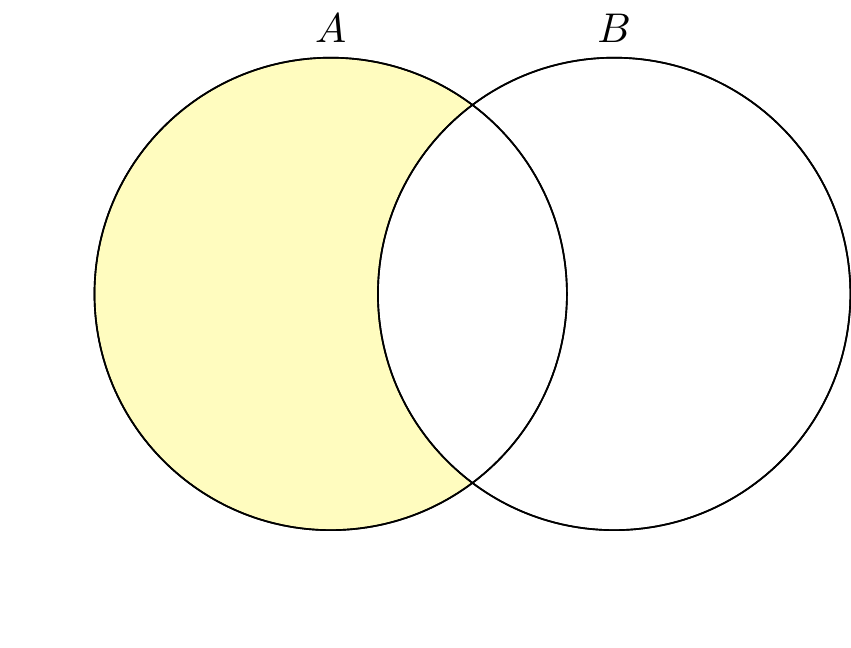
\includegraphics{introTextbookTemplate_files/figure-latex/unnamed-chunk-30-1} \end{center}

As we can see, these two curves are quite similar, and indeed, the underlying process that created each of them is the same. What is different, however, are the parameters governing how the data were generated. With this in mind, we have three goals for the present chapter

\begin{enumerate}
\def\labelenumi{\arabic{enumi}.}
\tightlist
\item
  Understand how a distribution represents a random process that creates data that is then observed
\item
  Understand how the parameters of a distribution govern how the data is generated {[}and with what probability{]}
\item
  Be able to identify which distributions underlying a given real world random process.
\end{enumerate}

\begin{definition}
\protect\hypertarget{def:unlabeled-div-1}{}\label{def:unlabeled-div-1}

Definitions

\end{definition}

\textbf{Probability Distribution: } A method for assigning probabilities to all possible events

\textbf{Distribution Parameters: } Values associated with a probability distribution that determine how the data is generated

\hypertarget{flipping-coins}{%
\section{Flipping Coins}\label{flipping-coins}}

In the previous chapter, we examined the possible events and associated probabilities with flipping a fair coin three times. In particular, we noted the collection of possible events was given by

\[\mathcal{S} = \{HHH, HHT, HTH, THH, TTH, THT, HTT, TTT\},\]
and the respective probabilities for the number of heads were

\# Heads

Probability

0

1/8

1

3/8

2

3/8

3

1/8

In what ways might we formalize this as a process? We might start by identifying a few details about this experiment. First, we know that we are interested in coin flips, where each flip could be either one of two outcomes. We might also recognize that in this experiment we flipped a coin three times, with each flip having an equal probability of being Heads as it did Tails. In light of our previous discussion, which of these properties seem characteristic of a more general underlying process, and which of these could be changed while retaining the more general form? If we had flipped the coin 50 times, would the process be fundamentally different? Would this process be different if the probability of Heads was twice that of Tails?

What we have identified above is a data generating mechanism, or distribution, known as the \emph{binomial distribution}, in which each outcome is one of two states. In this example, the two states were Heads and Tails, but it could just as easily be described as success vs failure, adverse reaction vs non-adverse reaction, death vs non-death, etc.,. Most generally, we will consider the outcome to be either an ``event'' or a ``non-event.''

We next turn our attention the parameters of the distribution. As you may have guessed, there are two parameters associated with the binomial distribution, namely the number of observations (or flips), denoted \(n\), and the probability of a particular outcome being classified as an event, denoted \(p\). In our coin flipping example, flipping the coin three times gives us a parameter value of \(n = 3\). As we were interested in counting the number of Heads, we will call this our ``event,'' and note that it occurs with probability \(p = 0.5\). Together, these pieces define everything we need to know about a random process that follows a binomial distribution. Notionally, we write

\[ X \sim Bin(n, p)\]

or, ``the random variable \(X\) follows a binomial distribution with \(n = 3\) and probability of event \(p = 0.5\).'' Our coin flipping example would then be expressed as \(X \sim Bin(n = 3, p = 0.5)\), where \(X\) is our experiment.

\hypertarget{functional-representation-of-probability-distributions}{%
\section{Functional Representation of Probability Distributions}\label{functional-representation-of-probability-distributions}}

We turn our attention now to the practical problem of determining how we might relate the idea of a probability distribution to determine the actual probabilities of given outcomes. From our definition above, we see that at a minimum, all we need is a method to assign a probability to a given event; within these bounds, we have a number of options available.

Perhaps the most direct method of doing so consists of counting each of the possible outcomes by hand and determining their probabilities, which is precisely what was done when we identified \(\mathcal{S}\) and then counted the frequency in which different numbers of Heads occurred. This, of course, can become cumbersome quite quickly: with only \(n = 3\), we identified a total of 8 separate outcomes. If \(n\) were 4, this would increase to 16. One can quickly see the issue when considering an experiment in which the total number of coin flips was equal to \(n = 50\). This example was further made easier by the fact that each of the outcomes was equally likely; if the value of \(p\) was anything but \(0.5\), our task of assigning probabilities to these outcomes would have been significantly more challenging (see Chapter 4).

Another possibility involves the use of simulation, the justification for which is covered in more detail in another chapter. By simulating this experiment a large number of times, we can determine the relative probabilities by counting the relative frequency of each outcome, which saves us the trouble of having to compute them mathematically. Here, we simulate this experiment \(N = 10,000\) times, and record the total number of heads in each experiment, dividing by the total number of experiments to get our desired probability

Number of Heads

Fraction

Observed Probability

True Probability

0

1,284/10,000

0.1284

0.125

1

3,762/10,000

0.3762

0.375

2

3,738/10,000

0.3738

0.375

3

1,216/10,000

0.1216

0.125

Of course as we can see, simulations have their own limitations: they often require a large number of replications, and because of randomness, the observed probabilities will rarely be exactly equal to the true probabilities. Nonetheless, simulations prove to be exceedingly useful when our experiment is complicated, or if a known distribution function for our problem does not exist.

Our final method for specifying a probability distribution is with the use of a mathematical function, often referred to as a \textbf{probability distribution function} (pdf) or \textbf{probability mass function} (pmf), with the former reserved for continuous variables and the latter for those that are discrete. The binomial distribution, consisting of discrete outcomes, is specified with a pmf. For \(X \sim Bin(n, p)\), we have the following formula:

\[
P(X = x) = \binom{n}{x} p^x (1-p)^{n-x}
\]

where \(n\) and \(p\) are our distribution parameters, and \(X\) can take any of the values \(x = 0, 1, \dots, n\). Perhaps new to us here is the leading term in the expression above, \(\binom{n}{x}\), called the \emph{binomial coefficient}, which can be written as

\[
\binom{n}{x} = \frac{n!}{x!(n-x)!}
\]
where \(n! = n \times (n-1) \times \dots \times 2 \times 1\) (known as a factorial). In words, we might say \(\binom{n}{x}\) as ``\(n\) choose \(x\).'' While this may seem daunting at first, the need for it is quite reasonable. Consider again our coin flipping experiment, where the possible outcomes were listed as

\[
\mathcal{S} = \{HHH, HHT, HTH, THH, TTH, THT, HTT, TTT\}.
\]

If we are interested in determining the probability of observing two Heads, it is of note that there are a number of instances above in which two Heads occurs. We might ask ourselves, ``if we have \(n = 3\) flips, how many ways might we \emph{choose} \(x = 2\) heads?'' Writing this with our binomial coefficient, we find that

\[
\binom{3}{2} = \frac{3!}{2!(3-2)!} = \frac{3 \times 2 \times 1}{2 \times 1 \cdot(1 \times 1)} = \frac62 = 3,
\]
and indeed, 3 is precisely the number of outcomes in \(\mathcal{S}\) in which two Heads occur. Finally, using the pmf above, we can substitute in our distribution parameters \(n = 3\) and \(p = 0.5\) to find the distribution function that describes our experiment:

\[
P(X = x) = \binom{3}{x} (0.5)^x (1-0.5)^{3-x}
\]
{[}Exercise: verify that the probabilities returned by the binomial pmf match the true probabilities in the table above by plugging in values for \(X = \{0, 1,2,3\}\). {]}

\hypertarget{plotting-the-pmf}{%
\subsection{Plotting the PMF}\label{plotting-the-pmf}}

It is often useful to create a visual representation of a pmf as well. Doing so quickly gives us an idea of where data tend to aggregate and how the data are dispersed. Below are two plots representing two different sets of parameters for the binomials distribution. What do you notice in how they differ? How are they similar? What impacts do the different parameters have on the distribution of the data?

\begin{center}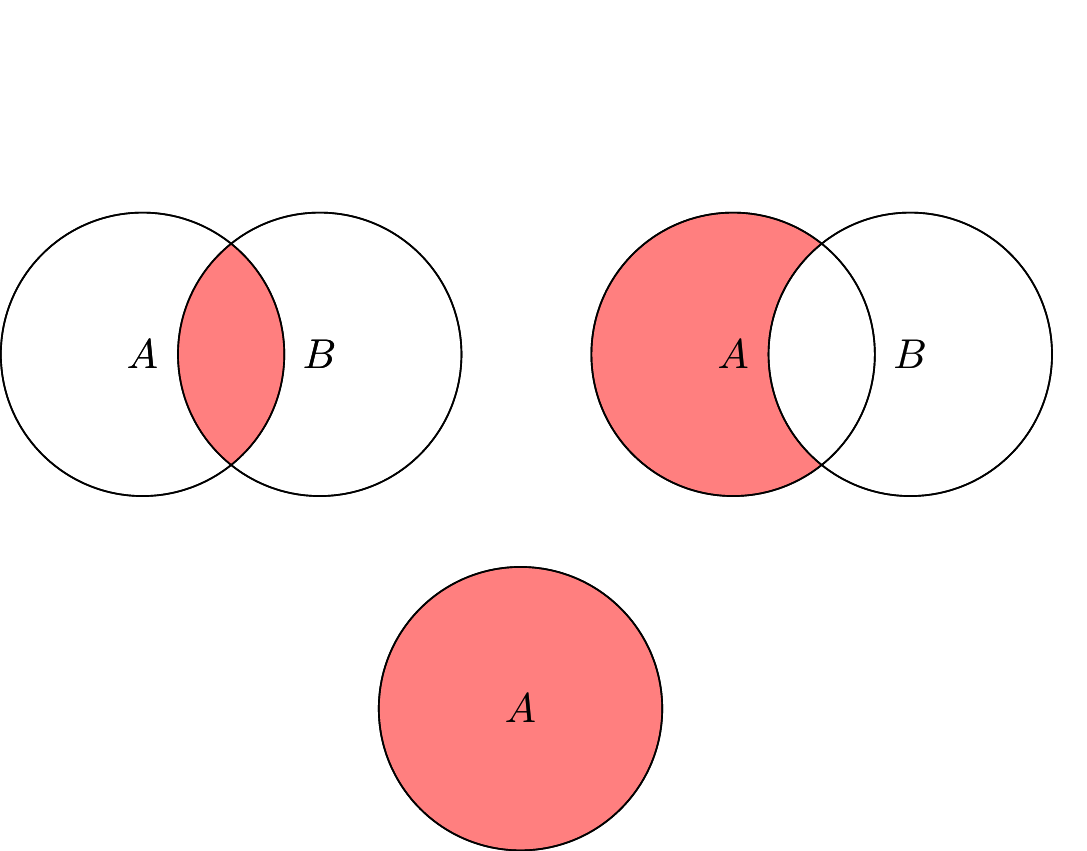
\includegraphics{introTextbookTemplate_files/figure-latex/unnamed-chunk-33-1} \end{center}

Of particular note here, we recall from the previous chapter that the sum of all possible probabilities must be equal to one. Visually, this is represented by the total area of the bars in our plot. Given that our bars our rectangles, we can find the area by considering that the width of each bar is equal to 1, and it's height is given by the probability of \(X = x\), which can be found using the PMF. On the left hand side, for example, from left to right, we have

\[
\begin{align}
\text{Total Area } &= \text{ \{Area of Heads = 0\} + \{Area of Heads = 1\} + } \\
& \quad \ \ \text{\{Area of Heads = 2\} + \{Area of Heads = 3\}} \\
&= (1 \times P(X = 0)) + (1 \times P(X = 1)) + (1 \times P(X = 2)) + (1 \times P(X = 3)) \\
&= 0.125+0.375+0.375+0.125 \\
&= 1
\end{align}
\]
If, say, we are interested in the probability that \(X = 2\) or \(X = 3\), we can add the area of the two corresponding bars. In this case, we find \(P(X = 2, 3) = 0.75\).

{[}Include binomial app here. See that clicking bars adds to something. Explain changing settings, clicking bars, selecting different things. Come up with exercises below, i.e., prob that even if n = 8, prob if even n = 4, etc.{]}

\hypertarget{measuring-heights}{%
\section{Measuring Heights}\label{measuring-heights}}

Often, our data will not fit nicely into a finite number of discrete categories, leaving us with \emph{continuous data} that are described with a \emph{probability distribution function}, or \emph{pdf}. As our data does not fit neatly into categorical bins, many of the techniques described above will not work in the same way here. Rest assured, the idea is exactly the same. While we will spare the technical details here, interested readers may consider what follows to be analogous to the cases presented above when the number of ``bins'' becomes infinite.

Our motivating example here will consider the process of determining the height of individuals within a population. Unlike the binomial distribution, where the underlying process and associated parameters were easily teased apart, the components here are less obvious, and some care will be needed to identify them. Height data, like many things in the natural world, tend to follow a symmetric distribution, where most observations tend to gather around a mean value, with observations deviating from the mean being equally likely to fall some distance above the mean as below, their frequencies becoming smaller as this distance increases. That is to say, if the mean height of a population is 68 inches, an individual is equally likely to be 67 inches tall as they are 69 inches. Similarly, an individual is equally likely to be 64 inches as they are 82. However, given their proximity to the mean value, an individual is far more likely to be either 67 or 69 inches (1 inch from the mean) than they are to be either 64 or 82 inches (4 inches from the mean).

The process described above describes what is known as a \emph{normal distribution}, colloquially referred to as a ``bell curve.'' There are a number of properties that together characterize a normal distribution

\begin{enumerate}
\def\labelenumi{\arabic{enumi}.}
\tightlist
\item
  There are two parameters for the normal distribution, the mean \(\mu\) (pronounced ``myu'') and the variance \(\sigma^2\) (``sigma squared'')
\item
  \(\mu\) is the mean, or expected value, and represents the most probable value of the distribution. That is, observations from a normal distribution are more likely to be close to \(\mu\) than away from it
\item
  Observations are equally likely to be the same magnitude above \(\mu\) as they are below it. In other words, the distribution is centered around \(\mu\). We see this concept expressed in everyday language when we offer estimates of some value: ``The cost is `x,' plus or minus `y'\,''
\item
  The second parameter, \(\sigma^2\), describes how concentrated values are around the mean. The smaller the value of \(\sigma^2\), the more observations that will be close to \(\mu\). Likewise, larger values of \(\sigma^2\) result in higher dispersion, or more values further away from \(\mu\).
\end{enumerate}

Notationally, if a random variable \(X\) follows a normal distribution with mean \(\mu\) and variance \(\sigma^2\), we write \(X \sim N(\mu, \sigma^2)\). A special case of this that will be explored in following chapters is known as a \emph{standard normal distribution}, which arises when the mean value is \(\mu = 0\), and the variances is \(\sigma^2 = 1\). This distribution is often written with its own letter \(Z\), as in \(Z \sim N(0, 1)\).

Another critical difference between a continuous and discrete random variable is the way in which we determine probability. In the discrete case, we could enumerate all of the events and determine their relative frequency. Alternatively, we could run a simulation and simply count how often each outcome occurred. In the continuous case, however, there is no finite set of possibilities (i.e., somebody could be 68" tall, 68.1" tall, 68.01", \ldots), and any attempts to enumerate these will only terminate in frustration; we will determine the implications of this below. In the meantime, however, we will rejoice in knowing that a normal distribution can be mathematically represented by it's probability function:

\[
f(x) = \frac{1}{\sqrt{2\pi \sigma^2}} \ e^{- \frac{(x-\mu)^2}{2\sigma^2}}
\]
As we can see, the pdf contains both of the distribution parameters, \(\mu\) and \(\sigma^2\). As we saw at the beginning of the chapter, different values for these parameters gives us different curves:

\begin{center}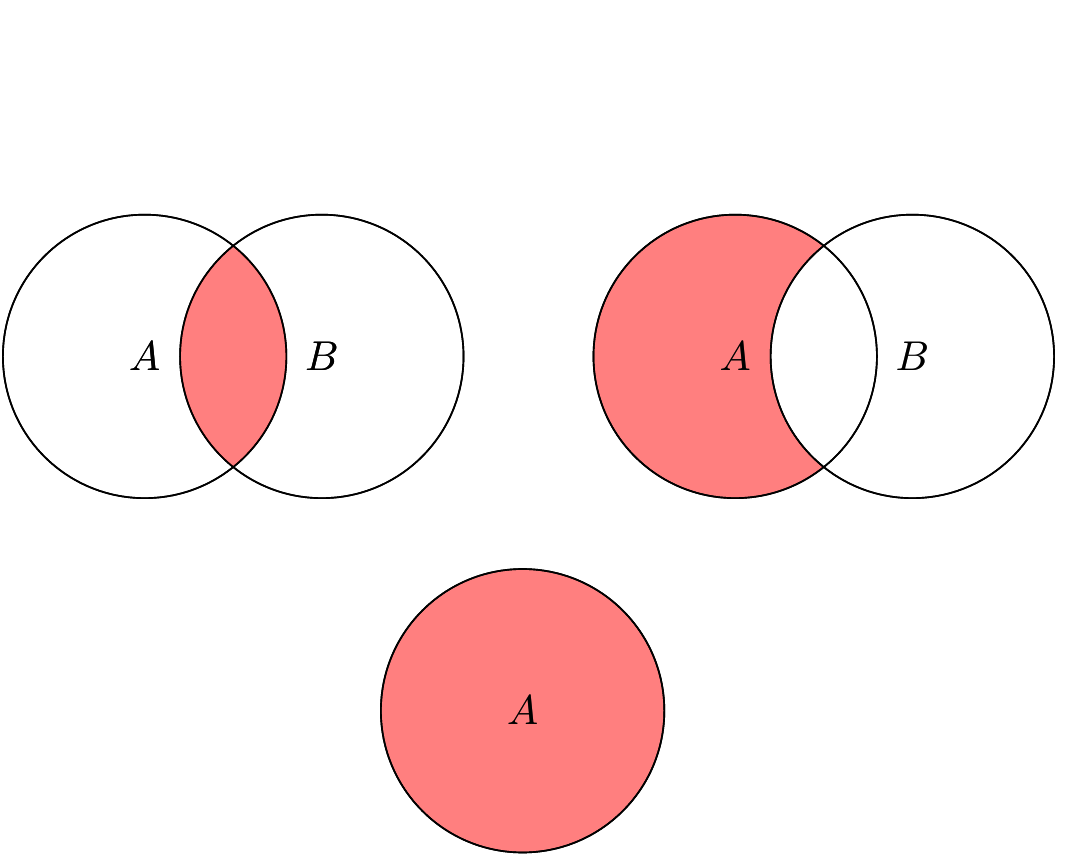
\includegraphics{introTextbookTemplate_files/figure-latex/unnamed-chunk-34-1} \end{center}

Of particular interest above, notice how the value of \(\mu\) changes where the data are aggregated, and similarly, note how larger values of \(\sigma^2\) results in a greater amount of dispersion.

Let's now return to the issue of determining the probability of a particular event. In the discrete case, we saw that we could examine the plot of the pmf and multiply the width of each bin (which was equal to 1), with the height of the bin, given by the pmf While the pdf here does indeed give us the ``height,'' we quickly run into an issue when considering the width: the only way we can have an ``infinite'' number of bins for each outcome is to assign each bin a width of 0. As such, the probability of any particular event is unintuitively assigned a probability of zero.

This apparent shortcoming can thankfully be remedied with the tools of calculus. Where discrete observations allow us to take a sum, the analogous case for continuous intervals is satisfied by the use of the integral. As it no longer makes sense to consider the probability of specific events (all of which will be zero), we instead consider the probability that an observation falls within a \emph{range} of events. For example, if we have a random variable with \(X \sim N(\mu, \sigma^2)\), the probability that \(X > 3\) can be written

\[
P(X > 3) = \int_3^{\infty} \frac{1}{\sqrt{2\pi \sigma^2}} \ e^{- \frac{(x-\mu)^2}{2\sigma^2}} \ dx
\]
Similarly, if we were curious to know the probability that \(X\) was between a range of values, say \(2 < X < 5\), we would write

\[
P(2 < X < 5) = \int_2^{5} \frac{1}{\sqrt{2\pi \sigma^2}} \ e^{- \frac{(x-\mu)^2}{2\sigma^2}} \ dx
\]
Fortunately for us today, this no longer need be computed by hand. A number of computational resources are able to compute this for us with minimal effort.

{[}Using app below, explore different parameter values. Use slider to select a range of probabilities. Note that the area of interest is highlighted. Do exercises with it{]}

\begin{definition}
\protect\hypertarget{def:unlabeled-div-2}{}\label{def:unlabeled-div-2}

Definitions

\end{definition}

\textbf{Binomial Distribution: } A discrete distribution in which there are two possible outcomes, ``events'' and ``non-events.'' There parameters are \(n\), which dictate the number of trials, and \(p\), determining the probability of an event

\textbf{Normal Distribution: } A continuous distribution with two parameters that is symmetric about a mean value, \(\mu\), with a variance \(\sigma^2\). Many real world processes follow a normal distribution.

\textbf{Standard Normal Distribution: } A special case of the normal distribution, \(Z \sim N(0, 1)\)

\textbf{Probability Mass Function: } A probability function used for discrete random variables. The probability of outcomes is given as a sum

\textbf{Probability Distribution Function: } A probability function used for continuous random variables. The probabilities of outcomes are taken over a range, given as an integral.

\hypertarget{other-common-distributions}{%
\section{Other Common Distributions}\label{other-common-distributions}}

Having examined in detail both discrete and properties distributions, demonstrated with the binomial and normal distributions, respectively, we consider below a brief overview of other common distributions and their properites.

\hypertarget{poisson-distribution}{%
\subsection{Poisson Distribution}\label{poisson-distribution}}

The Poisson distribution, like the binomial, is a \emph{discrete} distribution, in that it concerns itself with count data. Specifically, a Poisson distribution describes the number of independent events that may occur within a fixed interval of time. For example, we may be interested in the number of cars that pass through a busy intersection from noon to 1pm every day, or the number of major floods that occur in an area every 100 years. Perhaps the most famous example of the Poisson distribution comes courtesy of Ladislaus Bortkiewicz, a Russian statistician who, in 1898, showed that the number of Prussian soldiers killed by being kicked by a horse in a twenty year period followed a Poisson distribution (also child suicides, but that's less fun).

The Poisson distribution has a single parameter, \(\lambda\), which describes the rate at which events occur, and a random variable following a Poisson distribution may be expressed as \(X \sim Pois(\lambda)\) (People who write \(X \sim Po(\lambda)\) are heathens). A random variable following a Poisson distribution has the following assumptions:

\begin{enumerate}
\def\labelenumi{\arabic{enumi}.}
\tightlist
\item
  The value of \(X\), being a count, can be any non-negative integer, i.e., \(0, 1, 2, \dots\) with no upper bound
\item
  The occurrence of one event in a time interval is independent of another event. One soldier being kicked by a horse has no impact on the probability of another solider being kicked by a horse.
\item
  \(\lambda\), which may be any number greater than \(0\), describes the rate at which events occur
\item
  {[}Two events cannot occur at the exact same time, though they probably don't need this{]}
\end{enumerate}

The distribution function of a Poisson random variable with rate \(\lambda\) can be expressed

\[
P(X = x) = \frac{\lambda^x e^{-\lambda}}{x!}
\]
One surprisingly detail about the Poisson distribution is the relationship between the mean and the variance. For both, we have that \(E(X) = Var(X) = \lambda\).

\hypertarget{plots-for-poisson}{%
\subsubsection{Plots for Poisson}\label{plots-for-poisson}}

As we look at the plot for the Poisson, we will notice one aspect in particular that distinguishes it from the plots of both the binomial and normal distributions: it is no longer symmetric. This is a consequence of the range of values that a Poisson random variable can take on. Whereas a binomial random variable was bounded between \(0\) and \(n\), the number of trials conducted, and where the normal distribution allowed any real number, the Poisson is bounded below by \(0\), while having no theoretical upper bound. Given below is a plot of the distribution with \(\lambda = 2\) and \(\lambda = 4\) (it's obvious here that choosing a specific value is inadequate. We can replace these plots with distribution exploration apps)

\begin{center}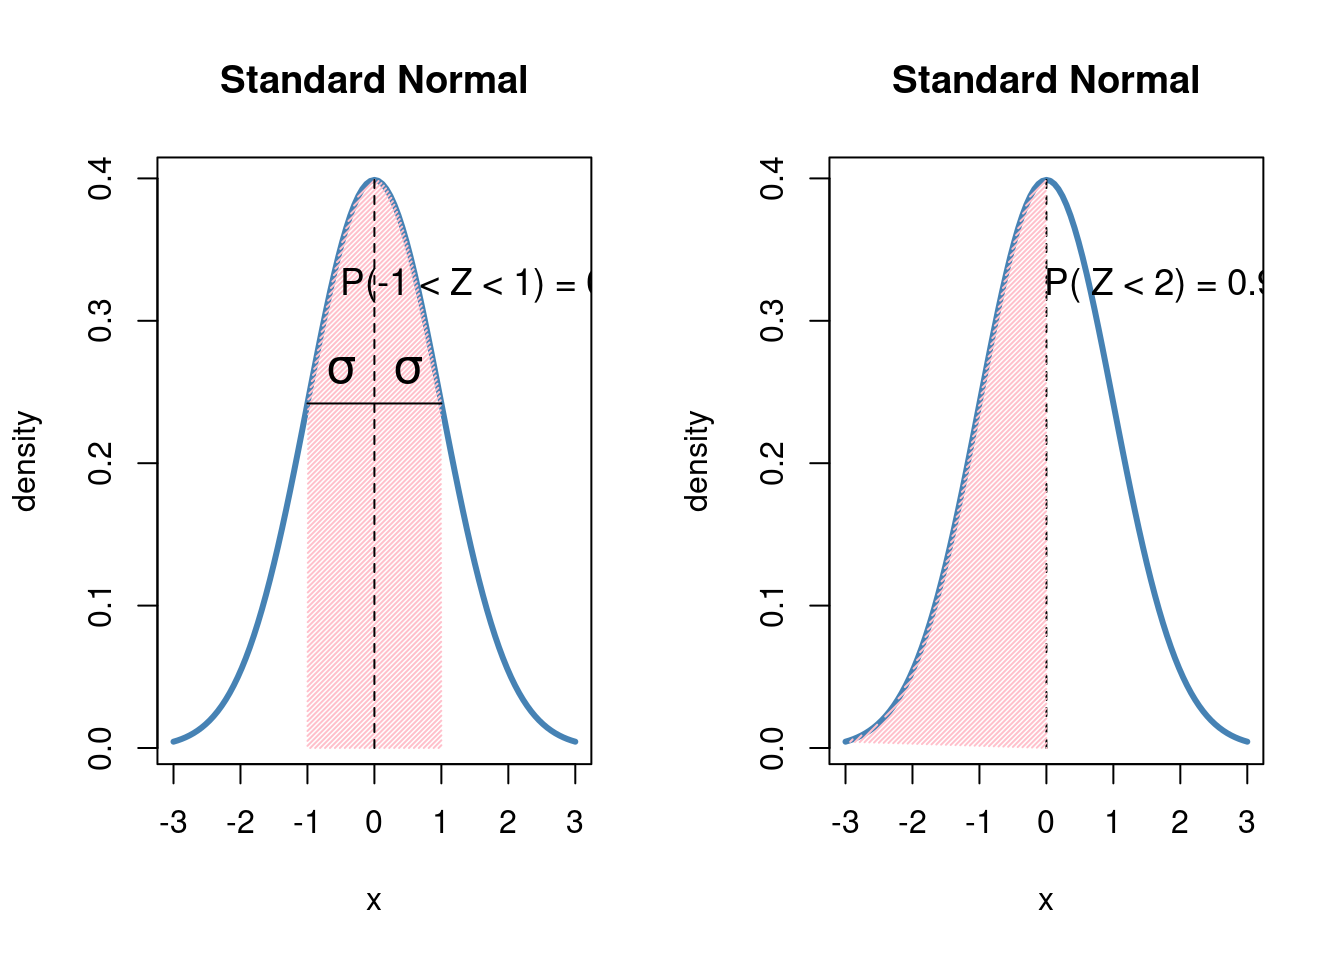
\includegraphics{introTextbookTemplate_files/figure-latex/unnamed-chunk-35-1} \end{center}

Just as with the binomial distribution, we can determine the probability of an event or collection of events by determining the area of the bars in our plot. Below is an interactive app to do stuff. Exercises

\hypertarget{ch6}{%
\chapter{\texorpdfstring{Sampling Distributions and the Central Limit Theorem}{Sampling Distributions and the   Central Limit Theorem}}\label{ch6}}

\begin{quote}
``While nothing is more uncertain than a single life, nothing is more certain than the average duration of a thousand lives.'' - Elizur Wright
\end{quote}

\begin{quote}
``Everything that can be counted does not necessarily count; everything that counts cannot necessarily be counted.'' - Albert Einstein
\end{quote}

Learning objectives

\begin{enumerate}
\def\labelenumi{\arabic{enumi}.}
\tightlist
\item
  Learn to differentiate between statistics and parameters\\
\item
  Understand the concept of sampling distributions\\
\item
  Conceptual understanding of Central Limit Theorem and how it applies to sample means
\end{enumerate}

\hypertarget{introduction-to-sampling}{%
\section{Introduction to Sampling}\label{introduction-to-sampling}}

Suppose policy makers and public health experts in Iowa are concerned with Iowans' fast food intake. To understand this further, officials want to determine the average monthly spending on fast food for all Iowans. However, it would be very expensive to have all 3.2 million Iowans track and report their total monthly fast food expenses. Whatsmore, many Iowans would not be willing to share personal financial details with public health researchers or government officials. These are but a few of the challenges making it practically impossible for officials to ever determine the true average spent by Iowans each month on fast food.

A true numeric quantity about the population, here assumed to be the mean, is known as a \textbf{population parameter}. While we may never know the truth, there are still options. The officials can take a sample of Iowans and have those that consent to share their information report their monthly spending on fast food. Then, they can take the sample mean, which gives them an estimate of the average monthly spending on fast food. The sample mean is an example of a \textbf{sample statistic}, which is a numerical quantity about the sample. In other words, statistics are what investigators know, and parameters are what investigators want to know.

The statistical framework (pictured below) allows us to make \textbf{inference} about population parameters using sample statistics. This means the researchers can use a random sample of Iowans' monthly fast food spending to make generalizations about the average monthly spending for all Iowans. The numerical quantities of interest can be many different things - means, proportions, standard deviations, etc.In the fast food example, the parameter of interest was a population mean and the sample statistic was the sample mean. In this chapter, we will specifically focusing on estimating means.

\begin{figure}

{\centering 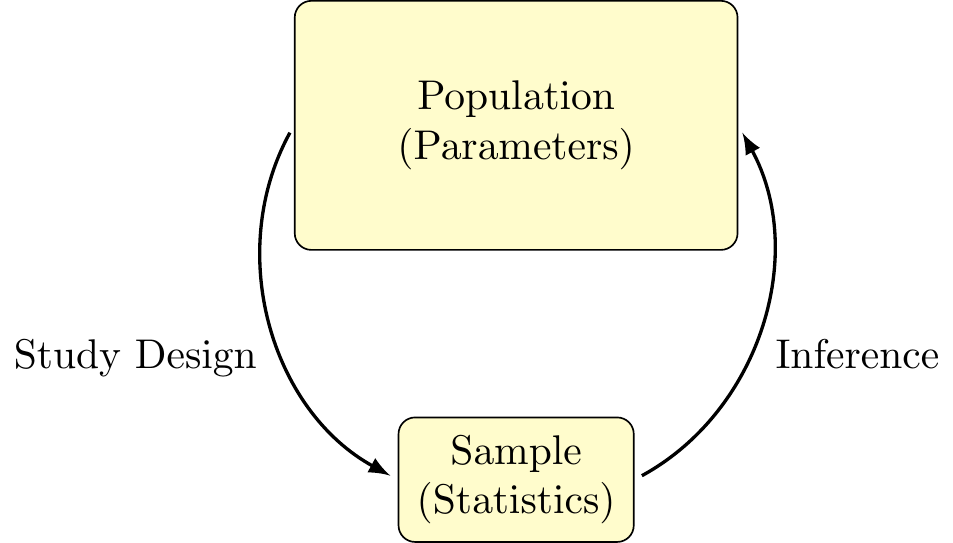
\includegraphics{introTextbookTemplate_files/figure-latex/statFramework2-1} 

}

\caption{Statistical Framework}\label{fig:statFramework2}
\end{figure}

The statistical framework outlines the process of making inference using sample statistics to estimate population parameters. Later chapters in this textbook will cover the mathematical details of this process. In trying to make proper inference, we also want to ensure our estimated statistic is measuring the parameter well. To that end, there are two major statistical issues we concern ourselves with:

\begin{itemize}
\tightlist
\item
  On average, does our estimate tend to be centered around the true answer, or is it \emph{biased}?\\
\item
  How much \emph{variability} is there likely to be in our sample?
\end{itemize}

The difference between our estimate and our parameter is called \textbf{bias}. \textbf{Variance} describes the spread of our data, and is sometimes called noise. Sometimes we talk about spread in terms of \textbf{precision}, which is the inverse of variance. The more precision we have, the less variance, and vice versa. A good statistic will have little or no bias and would have minimal variability. We can visualize both bias and variability using a dart board analogy.

\begin{figure}[H]

{\centering 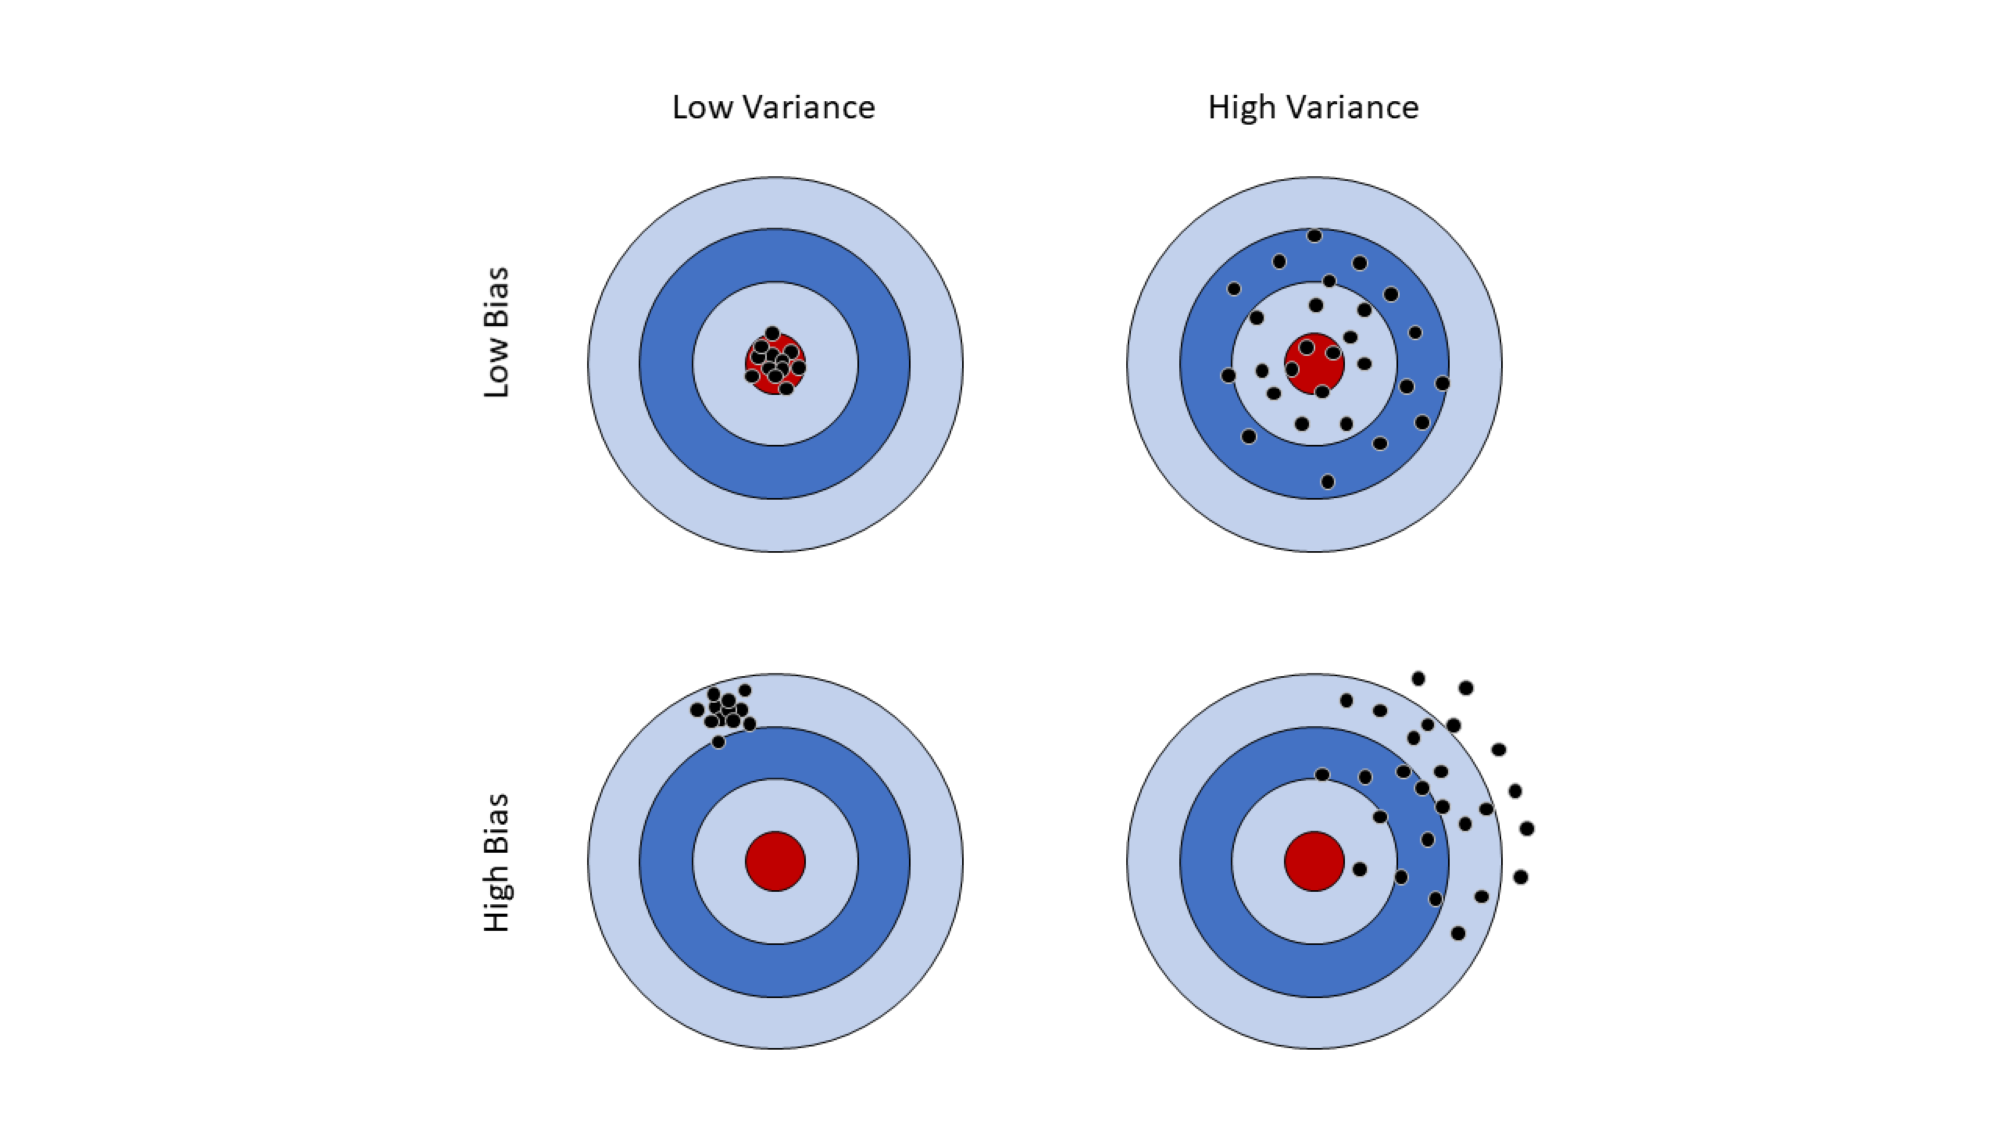
\includegraphics[width=27.78in]{./images/biasVariabilityTargets2} 

}

\caption{Bias and Variability Illustration}\label{fig:image-ref-for-in-text2}
\end{figure}

On the upper left target, the darts are hitting the bullseye with low bias and low variability, shown by the darts having minimal spread and all hitting the bullseye. This is the most desirable outcome when the goal is to hit the bullseye. In the upper right target, we see a lot more variability, as the darts are no longer highly concentrated on the bullseye. However, the dart locations are still centered around the bullseye, and this is why we consider this target to have low bias. This situation is less ideal than having low bias and low variance, but is still preferable to targets in the bottom row, where we have high bias. In the bottom left target, we have high bias and low variability, evidenced by the high concentration of darts that are not hitting the bullseye. The consistency is why we saw there is low variability, but if our goal is to hit the bullseye, we are not going to achieve that goal. Finally, the bottom right target is the worst possible outcome - high bias \emph{and} high variability. We are not hitting the bullseye and the darts are landing erratically. Statisticians work hard to develop inferential and sampling procedures that allow us to estimate population parameters with little to no bias and low variability.

\begin{definition}
\protect\hypertarget{def:unlabeled-div-3}{}\label{def:unlabeled-div-3}

Definitions

\end{definition}

\textbf{Population Parameter: } The true numeric quantity about a population

\textbf{Sample Statistic: } A numerical quantity about the sample

\textbf{Inference: } The process of making generalizations about the population

\textbf{Bias: } The systematic difference between our estimate and our parameter

\textbf{Variability: } The spread or error in the data

\textbf{Precision: } Inverse of variance, how narrow the data is

\textbf{Precision: (altered def. narrow data maybe confusing?) } Inverse of variance, or how precisely our estimate matches the parameter

\hypertarget{sampling-distributions}{%
\section{Sampling Distributions}\label{sampling-distributions}}

In order to make inference, we must be able to quantify our uncertainty about the population parameter based on our sample data. To quantify our uncertainty, we must first establish where it comes from - the sampling process. Any time we take a sample from the population, we will get a different sample mean \(\overline{x}\). In other words, \(\overline{x}\) is a numeric quantity which assumes a value based on the outcome of a random experiment - the process of drawing a sample at random from the population. This should sound familiar - this is the definition of a random variable! We can use this logic for any statistic of interest. As we've described in the past, random variables have probability distributions. When the random variable is a statistic, this probability distribution is called the sampling distribution. Sampling distributions reflect which values of the statistic are likely and which values are improbable. As we will see later in this chapter, this uncertainty depends on how many individuals we sample and how variable the data we measure is.

\begin{exercise}
\protect\hypertarget{exr:unlabeled-div-4}{}\label{exr:unlabeled-div-4}

Exercises

\end{exercise}

The applet below is designed to help you get familiar with the concept of random sampling. The plot on the left side gives the population distribution. Each subject in the population is represented by one box, and the population consist of 26 people. The x-axis represents the value of the outcome variable for each individual, and when multiple people have the same value, their boxes are stacked on top of each other. For example, we have one subject in the population with a value of 0, three subjects with values of 1, and so on. The plot on the right displays the values for the subjects in our sample, and these subjects are indicated by green coloring in both the population and sample distributions. We can take samples from our population of various sizes by changing the value of the slider at the top and clicking on the ``Sample'' button.

Set the sample size to 2 and click the ``Sample'' button five times. Fill out the following table with the sample means observed in your five samples.

Sample Number

Sample mean

1

2

3

4

5

Did you get the same sample mean for any of your five samples?

Was the sample mean ever equal to the population mean in any of your five samples? If not, how close were your sample means to the true population mean?

Now set the sample size to 15 and click the ``Sample'' button five times. Fill out the following table with the sample means observed in your five samples.

Sample Number

Sample mean

1

2

3

4

5

Did any of your five simulations give you a sample mean equal to the population mean?

how close were your sample means to the true population mean?

Compare your results from problem 1 and problem 2.

In either case were you able to obtain a sample mean equal to the population mean?

Which one had sample means with more variability? What does this indicate about the relationship between the sample size and the distribution of sample means in the context of repeated sampling?

As we've seen earlier in this book, we will use upper-case letters to denote random variables, and lower-case letters to denote values once they have been observed (that is, they are no longer random). When it comes to the sampling distribution of the mean, \(\overline{X}\) is the random variable, which arises from repeated random sampling from the population and then taking a sample mean, and \(\overline{x}\) is an observed sample mean we might see. In describing a sampling distribution, we are often interested in the mean and standard deviation - this gives information about typical values the statistic might take on as well as how spread out the distribution is. We refer to the mean of a statistic as the \textbf{expected value} and the standard deviation as the \textbf{standard error}. For the random variable describing the sample mean, these are denoted as \(E(\overline{X})\) and \(SE(\overline{X}) = \sqrt{Var(\overline{X})}\), respectively.

Let's return to the fast food scenario to motivate our development, but for now let's assume there are only five individuals in the entire population. The monthly spending for those five individuals (rounded to the nearest dollar) is as follows:

Person

Monthly Spending

A

8

B

22

C

22

D

36

E

50

The population mean can be found by taking the average monthly spending of these five individuals, as they are the only people in this population. This means the population mean is 27.6. Now suppose we are taking samples of three individuals from this population. There are \(\binom{5}{3}\) = 10 ways we can sample three people from this population. Since this is a small population, we can enumerate all possible samples, the values we would obtain for the monthly spending in each sample, and then the sample mean monthly fast food spending for each sample:

Sample

Values

\(\overline{x}\)

(A, B, C)

(8, 22, 22)

17.33

(A, B, D), (A, C, D)

(8, 22, 36), (8, 22, 36)

22.00

(A, B, E), (A, C, E), (B, C, D)

(8, 22, 50), (8, 22, 50), (22, 22, 36)

22.00

(A, D, E), (B, C, E)

(8, 36, 50), (22, 22, 50)

26.67

(B, D, E), (C, D, E)

(22, 36, 50), (22, 36, 50)

36.00

One thing to note is that \emph{none} of the sample means are actually equal to the population mean. This is often the case! Based on this table, we can construct the sampling distribution of \(\overline{X}\) for a sample of size three.

\begin{infobox}thinkaboutit

Why is our sample mean often not equal to the population mean?

\end{infobox}

Probability

P(\(\overline{x}\) = 17.33)

0.1

P(\(\overline{x}\) = 22)

0.2

P(\(\overline{x}\) = 26.67)

0.3

P(\(\overline{x}\) = 31.33)

0.2

P(\(\overline{x}\) = 36)

0.2

With this probability distribution, we can get the expected value of the sampling distribution. Whenever we think about probability, we are thinking about long-run frequencies, so when we think about the expected value, we are thinking about the average sample mean if we were to take repeated samples of size three from this population. The probability distribution indicates that if we took samples of size three from this population over and over again (say 1,000 times), we would end up with 10\% with a mean of 17.33, 20\% with a mean of 22, 30\% with a mean of 26.67; and so on. So the expected value (average) we would observed if we kept taking samples over and over would be:

(0.1 \(\times\) 17.33) + (0.2 \(\times\) 22) + (0.3 \(\times\) 26.67) + (0.2 \(\times\) 31.33) + (0.2 \(\times\) 36) = 27.6

But wait! That \emph{is} the population mean. This illustrates an extremely powerful property of the sample mean - the expected value of the sample mean \(\overline{X}\) is equal to the population parameter \(\mu\)! Because of this, we say that the sample mean is an \textbf{unbiased estimator} of the population mean. While we illustrated the property with a small example, this holds regardless of the population or sample size.

\begin{definition}
\protect\hypertarget{def:unlabeled-div-5}{}\label{def:unlabeled-div-5}

Definitions

\end{definition}

\textbf{Expected Value: } The mean value of a statistic in repeated sampling

\textbf{Standard Error: } The standard deviation of a statistic (including the mean) in repeated sampling

\textbf{Unbiased Estimator: } The statistic with an expected value equal to the true population parameter

\hypertarget{central-limit-theorem}{%
\section{Central Limit Theorem}\label{central-limit-theorem}}

In the last section, we used a toy example to conceptualize repeated sampling and the property of the sample mean being an unbiased estimator. Now we will formalize these properties. For \emph{any} population distribution which can be described by a random variable \(X\) with mean \(\mu\) and variance \(\sigma^2\), the sample distribution of the mean based on sample of size \(n\), denoted \(\overline{X}_n\), has the following properties:

\begin{enumerate}
\def\labelenumi{\arabic{enumi})}
\tightlist
\item
  The expected value of the sampling distribution is \(\mu\)
  \[E(\overline{X}_n) = \mu\]
\item
  The variance of the sampling distribution is
  \[Var(\overline{X}_n) = \frac{\sigma^2}{n}\]
\end{enumerate}

Using these formulas we are able to describe the typical value of the sample mean and how variable the sample mean is in repeated sampling. Notice that the expected value does not depend on the sample size, \(n\), but the variance does. This means regardless of the sample size, the sample mean is an unbiased estimator of the population mean. But, as the sample size increases, the variance decreases, and we get a more precise estimate of the population mean. As we've seen in the past, it is more common to talk about the standard deviation than the variance and the standard deviation is the square root of the variance. The quantity \(\sqrt{Var(\overline{X}_n)} = \sigma / \sqrt{n}\) is primarily called the \textbf{standard error} of the mean, and is denoted by \(SE(\overline{X}_n)\). We use the term standard error to make it really clear that it is referencing the sampling distribution of the mean, but all standard errors could be referred to as standard deviations. Conversely, not all standard deviations could be referred to as a standard error - the term is only used in describing the distribution of the sample mean.

In addition to knowing the mean and standard error of our statistic, we can also describe the \emph{distribution} of sample means in repeated sampling. As we discussed in the last chapter on probability distributions, a distribution for the sample mean provides us with a way to quantify which sample mean values are likely and which values are unlikely. As it turns out, when we repeatedly sample from a population, and continue to calculate the sample mean from each sample, the distribution of the sample means will be normally distributed. This brings us what is largely considered the ``fundamental theorem of statistics''

\textbf{Central Limit Theorem}

If the sample size is ``large,'' the sampling distribution of \(\overline{X}\) is approximately normal, regardless of the characteristics of the underlying population.

\[\overline{X}_n \sim N(\mu, \sigma^2/n)\]

While the term ``large enough'' will inevitably depend on the context of the problem at hand, a typical rule of thumb puts this value at \(n \geq 30\). Because the variance of \(\overline{X}\) is inversely related to the sample size, as the \(n\) increases, the variance decreases and the distribution becomes more concentrated around its mean value. This is one of the most important, remarkable, and powerful results in all of statistics. In the real world, we rarely know the underlying population distribution of our data, however, the Central Limit Theorem (CLT) says: we don't have to!

\begin{exercise}
\protect\hypertarget{exr:unlabeled-div-6}{}\label{exr:unlabeled-div-6}

Exercises

\end{exercise}

The applet below is designed to help your conceptual understanding of the CLT. You can change the underlying population distribution, the size of the samples taken (\(n\)), and the number of experiments performed. Each experiment consists of taking a sample of the specified size from the population and calculating the sample mean. The top left panel (blue) shows the underlying population distribution. The top right panel (red) shows the data from the most recent sample, with the sample mean from that specific sample indicated by the dashed black line. The bottom panel (gold) shows us the distribution of sample means from all the experiments, with the observed mean of the sample means indicated by the dashed black line and the true underlying population mean indicated by the solid blue line. Once you select the parameters to the values you want, click ``Run Simulation'' to tabulate the results.

Set the population distribution to Normal, the sample size to 30, and perform 100 experiments to collect 100 sample means.

Describe the histogram of the the data from the last experiment. Comment on the modality and skew.

Describe the histogram of the distribution of sample means from all experiments.

What is the range of values observed for the distribution of sample means? How does this compare the the range of values observed in the data from the last experiment?

Now adjust the sample size to 100. Perform 100 experiments.

What is the range of values observed for the distribution of sample means? How does this compare to the range observed when the sample size was 30?

What about the range of values observed in the data from the last experiment - did this change much when the sample size was increased?

Play around with various sample sizes. How does changing the sample size effect the spread of the distribution of sample means?

Return to a sample size of 30, but change the population distribution to be right skewed. Perform 1,000 experiments.

Describe the histogram of the the data from the last experiment. Comment on the modality and skew.

Describe the histogram of the distribution of sample means from all experiments. Does it resemble the population distribution?

Re-run the simulation using a sample size of 10. How does this effect the distribution of the sample means? How does this compare to what you observed when taking samples of size 10 with a normal population distribution?

Change the population distribution to be left skewed, set the sample size to 80, and perform 1,000 experiments.

Describe the histogram of the the data from the last experiment. Comment on the modality and skew.

Describe the histogram of the distribution of sample means from all experiments. Does it resemble the population distribution?

Run the simulation with these parameters a few times and pay attention to how the mean of the distribution of sample means compares to the population mean. Is the population mean similar or different from the mean of the sample means? What property does this illustrate?

Change the parameters of the simulations as needed to answer the following true/false questions. Explain your answers.

CLT tells us that the distribution of data from any experiment will be normally distributed.

With a larger sample size, the data from the last experiment will resemble the population distribution.

Performing 10 experiments is enough to see the effect of CLT.

Regardless of the underlying population distribution and the sample size, the distribution of the sample means will be normally distributed.

Increasing the sample size causes the data from a single experiment to look more and more normally distributed.

\hypertarget{ch8}{%
\chapter{Tests for Means}\label{ch8}}

\begin{quote}
``The only relevant test of the validity of a hypothesis is comparison of its predictions with experience.'' - Milton Friedman
\end{quote}

Learning objectives

\begin{enumerate}
\def\labelenumi{\arabic{enumi}.}
\tightlist
\item
  Steps for hypothesis tests
\item
  Learn how to perform one and two-sample tests for means
\end{enumerate}

\hypertarget{ch8_s1}{%
\section{Steps for hypothesis testing}\label{ch8_s1}}

Much of the rest of this book focuses on implementing hypothesis tests for various research questions and data types. While each hypothesis test is slightly different in the mathematical details and specific hypotheses being compared, the general procedure does not change. We consider hypothesis tests to have three primary steps:

\begin{enumerate}
\def\labelenumi{\arabic{enumi}.}
\item
  Things about the population
\item
  Things about the sample
\item
  Relate sample things to population (make inference)
\end{enumerate}

Let's dive a little deeper into each step.

\hypertarget{things-about-the-population}{%
\subsection{Things about the population}\label{things-about-the-population}}

Before doing any calculations, we first want to make sure we can describe the research question, the parameter(s) of interest, and can concretely write the null and alternative hypotheses.

\hypertarget{things-about-the-sample}{%
\subsection{Things about the sample}\label{things-about-the-sample}}

Once we set up our research question and the competing hypotheses, we can use the sample data to assess which hypothesis is more plausible. First we want to look at what we observed, i.e.~what are the estimates of the population parameters of interest. Then we use the sample data to calculate a p-value, which gives us the probability of observed something as extreme or more extreme than what we observed, given that the null hypothesis is true.

\hypertarget{making-inference}{%
\subsection{Making inference}\label{making-inference}}

Finally, we want to use the p-value computed from the sample data to make inference about the population parameter(s). Since the p-value quantifies the likelihood of our observations given the null hypothesis is true, a low p-value indicates evidence against the null and a larger p-value does not give evidence against the null. Based on whether the null hypothesis is rejected or not, we can answer the stated research question.

\hypertarget{ch8_s2}{%
\section{Hypothesis test for a mean}\label{ch8_s2}}

The first type of hypothesis test we will cover in detail is a hypothesis test for a mean. This test is used when we have one sample of continuous data, for which we feel comfortable summarizing the ``typical'' value with the mean. We seek to compare that mean to some known or pre-specified value to learn something about the population.

\begin{Shaded}
\begin{Highlighting}[]
\NormalTok{oneSampleMean }\OtherTok{\textless{}{-}} \ControlFlowTok{function}\NormalTok{(n, mean0, mean1, sd) \{}
\NormalTok{  obsDat }\OtherTok{\textless{}{-}} \FunctionTok{rnorm}\NormalTok{(n, mean0, sd)}
  
  \FunctionTok{hist}\NormalTok{(obsDat)}
  \FunctionTok{abline}\NormalTok{(}\AttributeTok{v =}\NormalTok{ mean1, }\AttributeTok{col =} \StringTok{\textquotesingle{}red\textquotesingle{}}\NormalTok{, }\AttributeTok{lwd =} \DecValTok{2}\NormalTok{)}
\NormalTok{\}}

\FunctionTok{oneSampleMean}\NormalTok{(}\DecValTok{100}\NormalTok{, }\DecValTok{5}\NormalTok{, }\DecValTok{4}\NormalTok{, }\DecValTok{1}\NormalTok{)}
\end{Highlighting}
\end{Shaded}

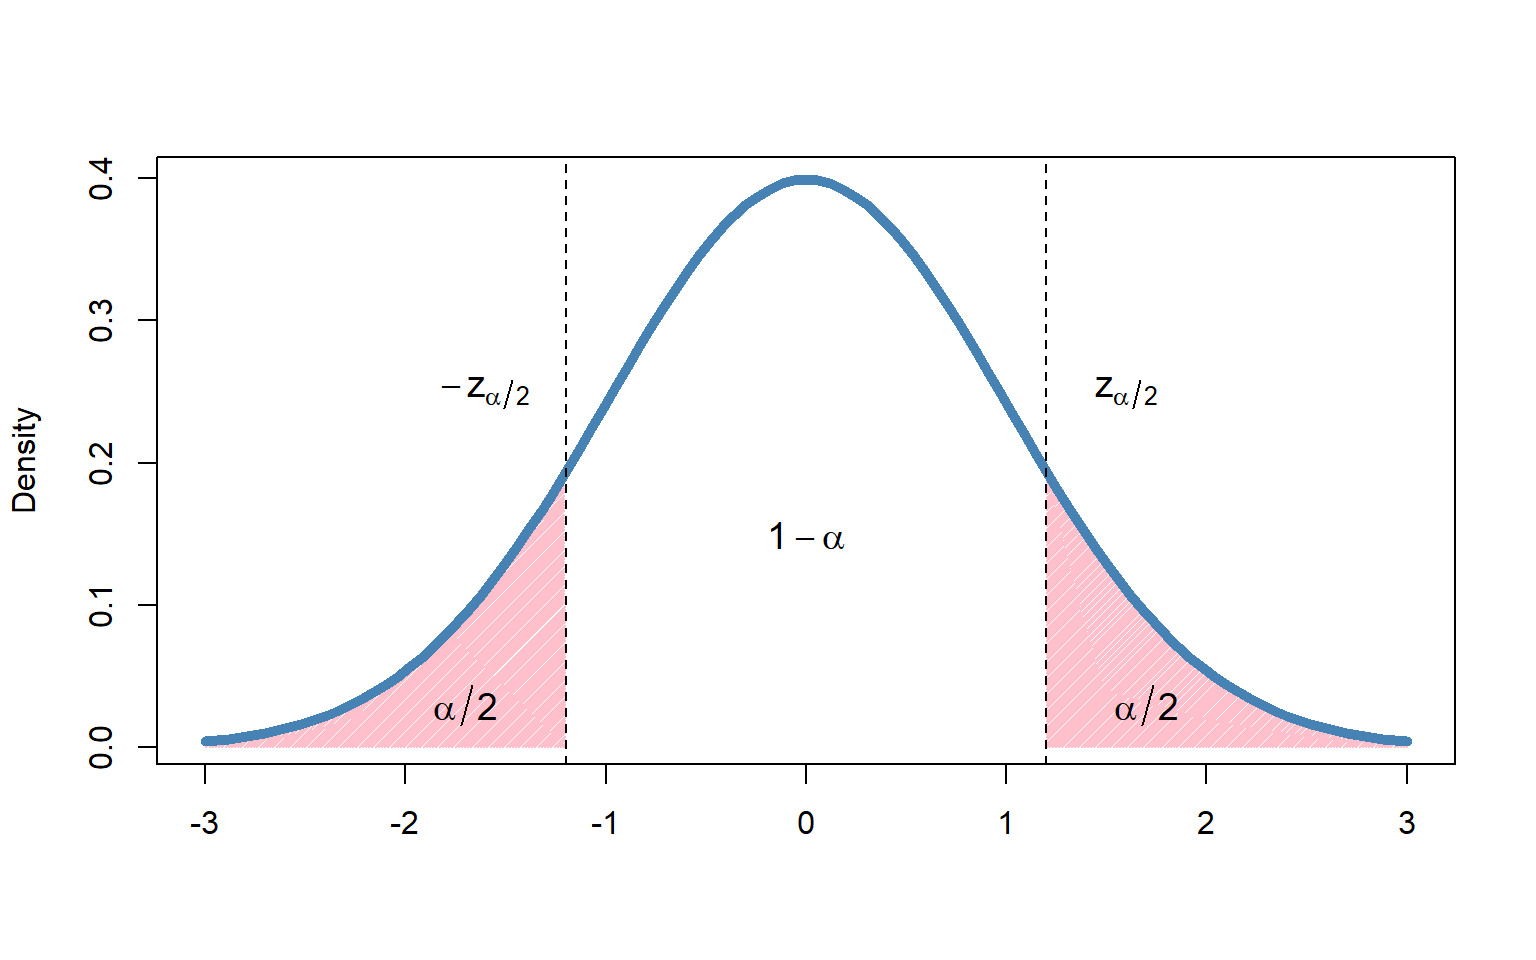
\includegraphics{introTextbookTemplate_files/figure-latex/unnamed-chunk-39-1.pdf}

\begin{Shaded}
\begin{Highlighting}[]
\NormalTok{twoSampleMean }\OtherTok{\textless{}{-}} \ControlFlowTok{function}\NormalTok{(n1, n2, mean1, mean2, sd1, sd2, }\AttributeTok{plot =}\NormalTok{ F) \{}
\NormalTok{  y1 }\OtherTok{\textless{}{-}} \FunctionTok{rnorm}\NormalTok{(n1, mean1, sd1)}
\NormalTok{  y2 }\OtherTok{\textless{}{-}} \FunctionTok{rnorm}\NormalTok{(n2, mean2, sd2)}
  
  \ControlFlowTok{if}\NormalTok{ (plot }\SpecialCharTok{==} \ConstantTok{TRUE}\NormalTok{) \{}
\NormalTok{    minVal }\OtherTok{\textless{}{-}} \FunctionTok{min}\NormalTok{(}\FunctionTok{c}\NormalTok{(y1, y2)) }\SpecialCharTok{{-}} \DecValTok{1}
\NormalTok{    maxVal }\OtherTok{\textless{}{-}} \FunctionTok{max}\NormalTok{(}\FunctionTok{c}\NormalTok{(y1, y2)) }\SpecialCharTok{+} \DecValTok{1}
    
\NormalTok{    ax }\OtherTok{\textless{}{-}} \FunctionTok{pretty}\NormalTok{(minVal}\SpecialCharTok{:}\NormalTok{maxVal, }\AttributeTok{n =} \DecValTok{12}\NormalTok{)}
    
\NormalTok{    hgA }\OtherTok{\textless{}{-}} \FunctionTok{hist}\NormalTok{(y1, }\AttributeTok{breaks =}\NormalTok{ ax, }\AttributeTok{plot =} \ConstantTok{FALSE}\NormalTok{) }\CommentTok{\# Save first histogram data}
\NormalTok{    hgB }\OtherTok{\textless{}{-}} \FunctionTok{hist}\NormalTok{(y2, }\AttributeTok{breaks =}\NormalTok{ ax, }\AttributeTok{plot =} \ConstantTok{FALSE}\NormalTok{) }\CommentTok{\# Save 2nd histogram data}
    
\NormalTok{    c1 }\OtherTok{\textless{}{-}} \FunctionTok{rgb}\NormalTok{(}\DecValTok{173}\NormalTok{,}\DecValTok{216}\NormalTok{,}\DecValTok{230}\NormalTok{,}\AttributeTok{max =} \DecValTok{255}\NormalTok{, }\AttributeTok{alpha =} \DecValTok{80}\NormalTok{, }\AttributeTok{names =} \StringTok{"lt.blue"}\NormalTok{)}
\NormalTok{    c2 }\OtherTok{\textless{}{-}} \FunctionTok{rgb}\NormalTok{(}\DecValTok{255}\NormalTok{,}\DecValTok{192}\NormalTok{,}\DecValTok{203}\NormalTok{, }\AttributeTok{max =} \DecValTok{255}\NormalTok{, }\AttributeTok{alpha =} \DecValTok{80}\NormalTok{, }\AttributeTok{names =} \StringTok{"lt.pink"}\NormalTok{)}
    
\NormalTok{    ylimits }\OtherTok{\textless{}{-}} \FunctionTok{c}\NormalTok{(}\DecValTok{0}\NormalTok{, }\FunctionTok{max}\NormalTok{(}\FunctionTok{c}\NormalTok{(hgA}\SpecialCharTok{$}\NormalTok{counts, hgB}\SpecialCharTok{$}\NormalTok{counts)))}
    
    \FunctionTok{plot}\NormalTok{(hgA, }\AttributeTok{col =}\NormalTok{ c1, }\AttributeTok{ylim =}\NormalTok{ ylimits)}
    \CommentTok{\# Plot 1st histogram using a transparent color}
    \FunctionTok{plot}\NormalTok{(hgB, }\AttributeTok{col =}\NormalTok{ c2, }\AttributeTok{add =} \ConstantTok{TRUE}\NormalTok{)}
    \CommentTok{\# Add 2nd histogram using different color}
\NormalTok{  \}}
  
  \FunctionTok{c}\NormalTok{(}\FunctionTok{mean}\NormalTok{(y1), }\FunctionTok{mean}\NormalTok{(y2), }\FunctionTok{sd}\NormalTok{(y1), }\FunctionTok{sd}\NormalTok{(y2), n1, n2)}
  
\NormalTok{\}}

\FunctionTok{twoSampleMean}\NormalTok{(}\DecValTok{100}\NormalTok{, }\DecValTok{100}\NormalTok{, }\DecValTok{5}\NormalTok{, }\DecValTok{10}\NormalTok{, }\DecValTok{1}\NormalTok{, }\DecValTok{1}\NormalTok{, }\AttributeTok{plot =}\NormalTok{ T)}
\end{Highlighting}
\end{Shaded}

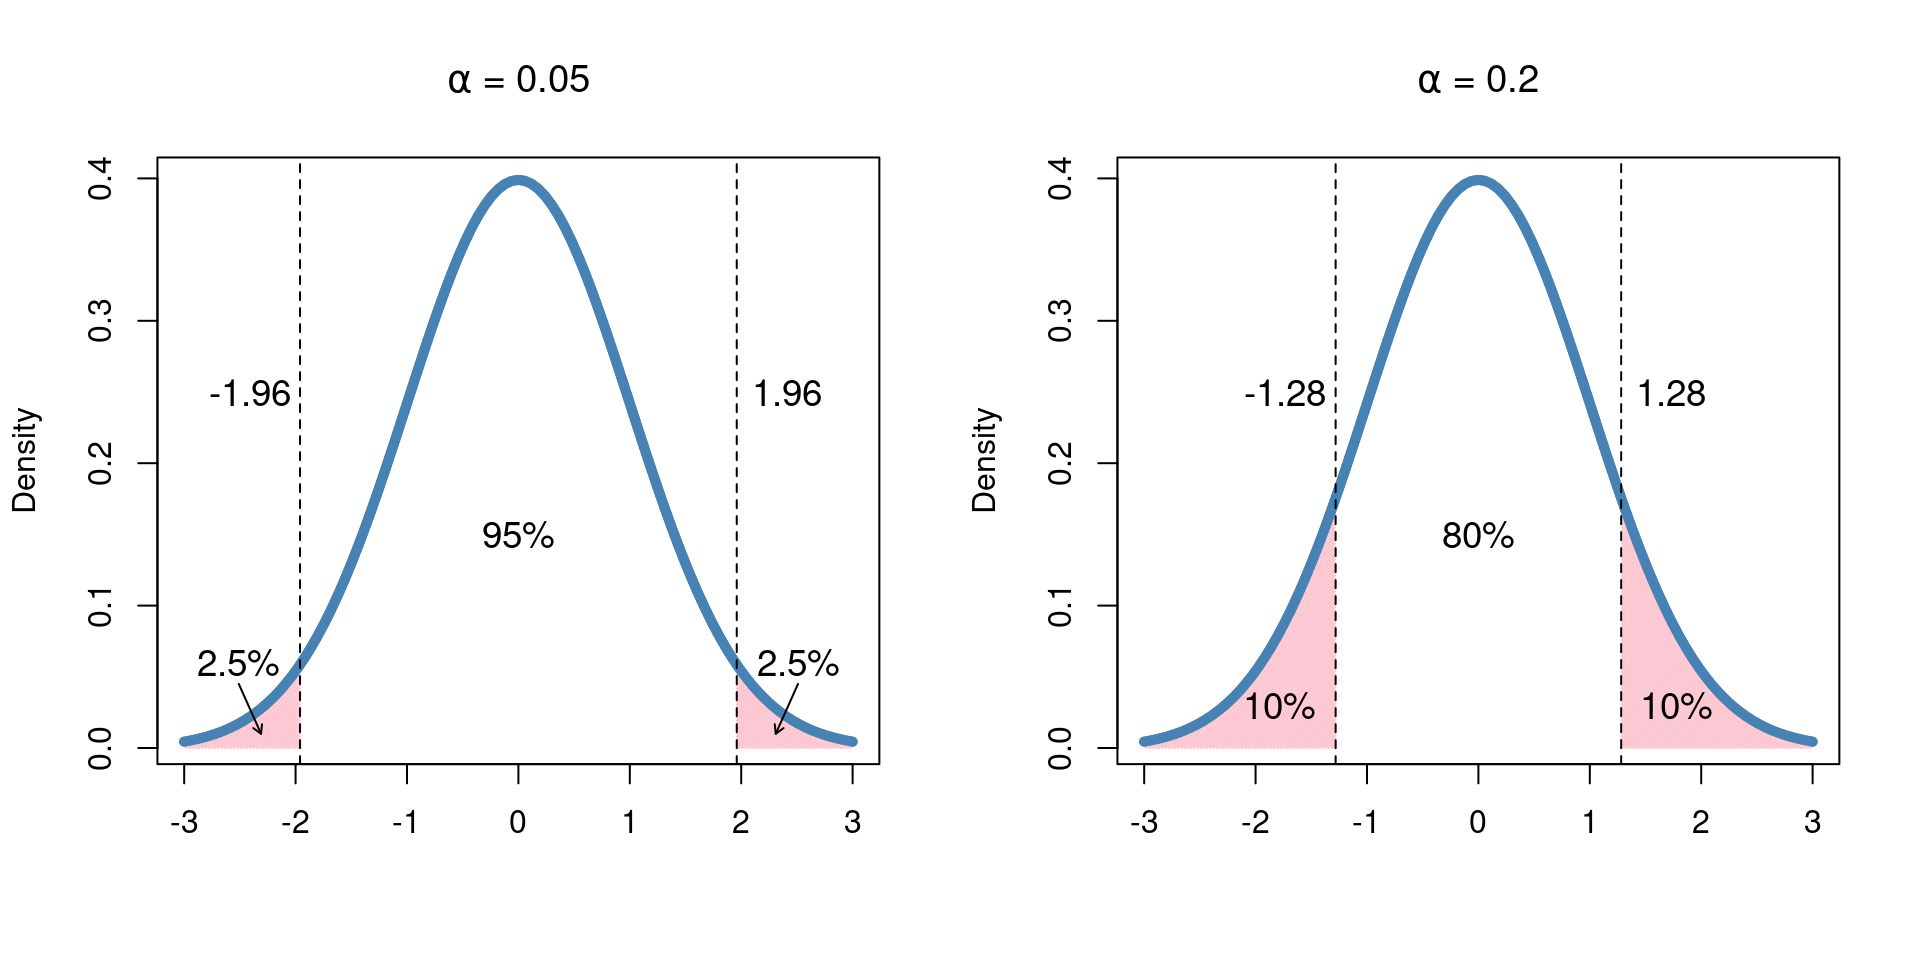
\includegraphics{introTextbookTemplate_files/figure-latex/unnamed-chunk-40-1.pdf}

\begin{verbatim}
## [1]   5.04431   9.90422   0.87857   1.04485 100.00000 100.00000
\end{verbatim}

\begin{Shaded}
\begin{Highlighting}[]
\NormalTok{repVals }\OtherTok{\textless{}{-}} \FunctionTok{replicate}\NormalTok{(}\DecValTok{10000}\NormalTok{, }\FunctionTok{twoSampleMean}\NormalTok{(}\DecValTok{100}\NormalTok{, }\DecValTok{100}\NormalTok{, }\DecValTok{5}\NormalTok{, }\DecValTok{10}\NormalTok{, }\DecValTok{1}\NormalTok{, }\DecValTok{1}\NormalTok{))}
\end{Highlighting}
\end{Shaded}

\hypertarget{ch9}{%
\chapter{Non-normal Continuous Data}\label{ch9}}

Learning objectives

\hypertarget{ch10}{%
\chapter{Categorical Data}\label{ch10}}

Learning objectives

Up until this point, the hypothesis tests we've covered have been tests about population means. In other words, the outcome measured was continuous. However, many times our variable of interest is categorical and requires a different method.

\hypertarget{ch10_s1}{%
\section{One Sample Proportions}\label{ch10_s1}}

For example, if researchers were interested in investigating the proportion of college students who binge drink, the researchers could ask a sample of students if they had engaged in binge drinking in the past month, and the students would answer yes or no. If the investigators had asked how many drinks they had had in the past month, then we might be interested in looking at the mean number of drinks. But, let's say they did not ask this question, and we have a categorical outcome.

When we have a sample, and each person is asked a yes or no question, we can describe the probability of their responses using a binomial distribution. In binomial distribution, there are two parameters, the sample size and the probability of an event occurring. Since the researchers are interested in proportion, they are actually interested in estimating the event probability.

\hypertarget{ch10_s2}{%
\section{Two Sample Proportions}\label{ch10_s2}}

\hypertarget{ch10_s3}{%
\section{Contingency Based tests}\label{ch10_s3}}

\hypertarget{ch10_s4}{%
\section{Paired Categorical Data}\label{ch10_s4}}

\hypertarget{ch11}{%
\chapter{Correlation and Regression}\label{ch11}}

Learning objectives

\hypertarget{ch12}{%
\chapter{Introduction to Simulations}\label{ch12}}

Learning objectives

\begin{enumerate}
\def\labelenumi{\arabic{enumi}.}
\tightlist
\item
  Understand what a simulation is
\item
  Understand why simulations are useful
\item
  Learn the types of illustrations that can be helpful to summarize simulations
\item
  Conceptual understanding of randomness and a simulation
\end{enumerate}

\hypertarget{ch12_s1}{%
\section{What is a simulation?}\label{ch12_s1}}

In the statistics world, when we use the word simulation we are not talking about
\emph{The Matrix} or \emph{Westworld,} where humans exist in some simulated reality. Statistical simulations
use a computer to observe potential results of an experiments. Simulations can be used
for experiments as simple as flipping a coin or as complicated as investigating the dynamics of human
movement and interaction. One thing that all simulations have in common is the element
of \textbf{randomness}. If there was nothing random, the process would result in the same
outcome every time - like if someone offered me an all-expenses paid trip to Hawaii - the
answer is always yes. This is what we call a \textbf{deterministic} outcome, and it is not
something where any statistical inference is needed. However, more often than not,
the phenomenon of interest is what we call \textbf{stochastic} which means there is
some element of randomness - like the weather in Hawaii during my trip - it might
be sunny, it might be rainy, and there is a tiny chance it might be below freezing.

Simulations allow us to specify the \textbf{parameters} that govern the scenario and then
with the help of a computer, we can watch the scenario play out over and over. In the end,
this gives us an idea of all the likely outcomes \emph{and} just how likely those outcomes might be.
Let's start with a simple example - flipping a coin

\hypertarget{ch13}{%
\chapter{Introduction to Simulations}\label{ch13}}

Learning objectives

\begin{enumerate}
\def\labelenumi{\arabic{enumi}.}
\tightlist
\item
  Understand what a simulation is
\item
  Understand why simulations are useful
\item
  Learn the types of illustrations that can be helpful to summarize simulations
\item
  Conceptual understanding of randomness and a simulation
\end{enumerate}

\hypertarget{ch13_s1}{%
\section{What is a simulation?}\label{ch13_s1}}

Throughout this text, we will often describe simulations in terms of coins and dice. While these examples may feel contrived, they do serve to illustrate the components of probability, randomness, and simulation in a way that is free from unnecessary complication. For example, flipping a coin has exactly two outcomes with equal probability; the goal here is not to bore you with unmotivating examples (``When am I ever going to flip 10,000 coins?'') but rather to allow the focus of the discussion to be on the conceptual elements -- \emph{experiments, events, outcomes, and probabilities}. Keeping this in mind will help the reader keep narrow center their focus on the relevant information, if at the slight expense of imaginative creativity.

For most of its history, nearly all of statistics were done in an analytic fashion, with the use of concise formulas and tedious calculation. However, with the ubiquity of modern computers, something something something

As an aid to our learning, we will be making heavy use of a tool known as simulation. In the broadest sense, computer simulations allow us to quickly and consistently repeat a random experiment that we might use to form conclusions about a process. Before going into technical details, let's begin with a simple random experiment that has a single event, the act of flipping a fair coin one time:

{[}{[}app{]}{]}

(too many colons and semicolons below)

Because this is a fair coin, we know before we flip it that there is an equal probability of it landing on either heads or tails. Because we are unsure of the outcome before hand, we say that the outcome is \emph{random} Once the coin is flipped, however, it is either heads \emph{or} tails; that is, once the result is no longer random, we say that it is \emph{observed}. This is a subtle but important distinction:

Processes (such as flipping a coin) in which randomness occurs are known as \textbf{stochastic processes}. By contrast, a process that is not random is known as \textbf{deterministic}, as the outcome is determined before hand. An example of a determinsitic process may include ordering a collection of numbers from largest to smallest: every time we are given the same collection of numbers, the resulting order will be the same. Our primary interest in this text will be the investigation of statistical processes, aided with the use of simulation.

It's worth taking a moment here to reflect on the somewhat obvious statement that we have not flipped an actual coin, but have instead performed a \emph{computer simulation}. There are (three) (more? different things? make part of definition?) components of our experiment that identify it as such (might also break this into parts not unique to simulation in general but coin flip in particular. then we can separate number of flips, number of coins, probability, etc)

\begin{enumerate}
\def\labelenumi{\arabic{enumi}.}
\item
  We specified the possible outcomes and the probability of each outcome occuring. In this case, our outcomes were heads and tails, each with a probability of 50\%.
\item
  We specified the number of coins we wanted to flip, as well as the number of times we wanted to flip them. For this simple example, we elected to flip a single coin one time.
\item
  We performed this experiment with the aid of a computer.
\end{enumerate}

While (3) may seem a trivial component of our definition, it has two important implications: we were able to exactly specify the criteria in (1) and (2), and we are able to repeat \emph{this exact same experiment} knowing that the initial set of conditions will remain exactly the same. The utility of this framework, or computer simulation, comes from the fact that we can conduct a random experiment as many times as we wish in the anticipation that by doing so, we can learn something about the behavior of random processes in general.

Let's now return to the coin flip simulation and investigate ways in which we can make our experiment slightly more complex. In the first implementation, we observed a single \textbf{event}, or observed outcome, resulting from the flip of the coin. Letting \(n\) represent the number of total events, we would say that this simulation was carried out with \(n = 1\). In the example below, we repeat the simulation above, but this time we are able to change the value of \(n\):

{[}{[}app{]}{]}

Just as before, while having defined \(n\) allows us to control the behavior of the simulation, it does not interfere with the effects of randomness. In other words, each time the simulation is run, a different outcome appears. Values such as \(n\) that change the behavior of the simulation are known as \textbf{simulation parameters}. We will consider a number of parameters that are commonly used to direct the simulation.

(this was rewritten above. not sure on appropriate order of concepts and definitions)

Once an outcome is complete and the coins have been flipped, we say that it is \textbf{observed}, or that \emph{we have observed the outcome of a random process}. Here, it is important to note that an observed outcome is no longer random -- once the data have been observed, we know what they are. Data collected through real life experiments, such as testing the efficacy of new drugs, or measuring the height of people in a population, are all observed data. As is often lamented by researchers and statisticians alike, real word experiments can often only be conducted a single time. Once the data is observed, it's observed. This is in stark contrast to the power of simulations, in which experiments can be conducted and data observed an arbitrary number of times.

To see this in action here, consider the previous example in which we introduced the simulation parameter \(n\), which allowed us to dictate the number of events, or coin flips, that were done in our experiment. Suppose the experiment that we are interested in involves flipping a coin three times: in this case, we have \(n = 3\). When we ran the simulation above, the experiment was done once, as is often the case in the real world, and we were left with a single collection of \emph{observed data}. It now makes sense to introduce a new simulation parameter, \(N\), which dictates \emph{how many times the experiment is to be done}. In this last instance, our simulation was done with \(N = 1\). In the simulation below, we will continue to run the experiment with three coin flips (\(n = 3\)), but we will change the number of times \(N\) that the experiment is run.

{[}{[}app{]}{]}

It is important to note that the experiment itself is unchanged -- just as before, we are continuing to investigate what happens when a coin is flipped \(n = 3\) times. By adjusting the value of \(N\), we are now able to perform this same experiment as often as we wish. Even more importantly, one sees that even though the exact same experiment is performed a number of times, the \emph{observed} values of the experiment are different. This is again a consequence of randomness, and demonstrates that even when we know all of the details of an experiment, the outcome is uncertain until it is observed.

\hypertarget{why-simulation}{%
\section{Why Simulation}\label{why-simulation}}

In the previous section, we learned that a simulation is a random process (of \(n\) events) that can be performed an arbitrary number of (\(N\)) times. Our next step will be to understand how this process can empower us to better understand key concepts in statistics. The next section will contain a number of terms and concepts that will be formally introduced in later chapters, but for now will serve to give context to the usefulness of simulations.

We will continue with the experiment above, where we are interested in flipping a fair coin \(n = 3\) times. However, along with the experiment, we will also bring a question: if a coin is flipped three times, what is the probability that exactly two of the coins will be heads? Before we attempt answering this via simulation, it will be instructive to consider first the ways we might answer it without.

{[}{[}might be nice to ``name'' these methods, like pdf method and something else.{]}{]}

\hypertarget{non-simulation-methods}{%
\subsection{Non-simulation Methods}\label{non-simulation-methods}}

We will start by introducing two non-simulation methods to answer this question, which we will call the \emph{enumeration method} and the \emph{probability function method}

Let's first consider the enumeration method. As \(n\) is small enough, we could simply list all of the possible outcomes of this experiment and count how many of these outcomes have exactly two heads. The space of outcomes for this experiment where the coin is flipped \(n = 3\) times, denoted \(\mathcal{S}\), is given by

\[
\mathcal{S} = \{HHH, HHT, HTH, THH, TTH, THT, HTT, TTT\}
\]
where \(H\) represents a heads and \(T\) a tails. Having listed them out, we see there are eight possible outcomes. Next, we count how many of those have exactly two heads:

\[
\mathcal{S} = \{HHH, \color{red}{HHT}, \color{red}{HTH}, \color{red}{THH}, TTH, THT, HTT, TTT\}
\]
Dividing the events of interest by the total number of outcomes, we see that the probability of getting exactly two heads is \(P(\text{# Heads = 2}) = \frac{\text{# Heads = 2}}{\text{# Possible Outcomes}} = \frac38\).

Often, a statistical or stochastic process has an associated \emph{probability function} that allows us to determine the probability of a set of outcomes. In this case, our coin flipping example follows what is known as a \emph{binomial distribution}, which is given as

\[
P(\text{# Heads = k}) = f(k; n,p) = \binom{n}{k}p^k(1-p)^{n-k}
\]
with probability of heads being \(p = 0.5\), \(n = 3\) total flips, and for our event, \(k = 2\) heads. Substituting these numbers, we have

\[
\begin{align*}
P(\text{# Heads = 2}) &= \binom{3}{2} (0.5)^2 (0.5)^{3-2} \\
&= 3 \times (0.5)(0.5)(0.5) \\
&= 0.375.
\end{align*}
\]
Just as in the enumeration method, we find that \(P(\text{# Heads = 2}) = 0.375 = \frac38\)

While each of these methods is satisfactory (and mathematically equivalent), there are a number of situations in which they would be impractical to perform:

\begin{enumerate}
\def\labelenumi{\arabic{enumi}.}
\item
  For example, in the first method, we determined the probability by counting the total number of events of interest (getting two heads) and dividing it by the total number of possible outcomes, in this case eight. For \(n = 4\), there are 16 possible outcomes, and for \(n = 10\), this number grows to 1024. In fact, the number of possible outcomes grows exponentially with the number of flips: with only \(n = 25\) coin flips, there would be more possible outcomes in our solution space than the number of hours between today and the construction of the Great Pyramid of Giza, c.2580-2560 BC. Clearly, we need a method that is a bit more concise
\item
  Our second method, determining probability via the probability function, is far and away the most popular method, as the computation is simple and immediate. Unfortunatley, we are limited by the crucial fact that we have to know what the probability function is in order to compute it. For many real life processes, such as flipping coins or estimating the number of phone calls a call center will receive in an hour, this function is readily known. For processes that are more complex, these functions can be nearly impossible to construct, leaving statisticians and researchers with no clear way to specify the probability of events.
\end{enumerate}

\hypertarget{simulation-method}{%
\subsection{Simulation Method}\label{simulation-method}}

Before moving forward, let's quickly recap where we are right now:

\begin{enumerate}
\def\labelenumi{\arabic{enumi}.}
\item
  Simulation is a tool that we have, governed by a set of parameters (in our case, \(n\) and \(N\)), that can be used to replicate a random experiment an arbitrary number of times. Because this process is \emph{stochastic}, or random, it will give a different outcome each time
\item
  We have specified an experiment we would like to perform, flipping a fair coin \(n = 3\) times, and we would like to know the probability that exactly two of the flips will land on heads. Together, these define our experiment and our research question
\item
  We investigated two methods besides simulation for answering this question: enumerating the event space and calculating the probability function. These methods gave identical answers, and will continue to do so each time they are performed: in other words, they are \emph{deterministic} methods for determining probability.
\item
  We saw that even though enumeration and probability functions worked fine for our problem, they can quickly become impractical or even impossible once the problem grows or becomes more complex
\end{enumerate}

{[}{[}paragraph below should be moved to later. what we should do first is rediscuss the problem above, do it in the context of simulation, and then verify that asymptotically we get the same answer. not yet sure best way to introduce/order this information{]}{]}

A careful reader might note that for a given random experiment (flipping a coin three times) and a specified outcome (exactly two heads), there is only a single correct answer to the question ``What is the probability of getting exactly two heads when flipping a coin three times?'' and this correct answer is precisely what was found using the deterministic enumeration and probability function methods. And if this is true, how could we possibly expect simulation, which gives us \emph{random} outcomes, to give us the same correct result? The answer lies in one of the most profound results in all of statistics, the \textbf{law of large numbers}. We will cover this in much greater detail in later chapters, but for now, it suffices to know that the law of larger numbers states: ``the average of the probabilities obtained from a large number of trials should be close to the true probability, and will tend to become closer are more trials are performed.'' In the context of our problem, we can restate this as ``as the number of experiments performed \(N\) becomes larger, the average of all the results will get closer and closer to the true result.'' Or more clearly still, ``our simulation will match determinstic methods when \(N = \infty\).'' That's pretty neat.

We will end this chapter with a demonstration of the claims made above. Verify that as \(N\) increases, the calculated probability from the simulation matches the analytic results made above. In addition, try changing the experiment and the outcome of interest. This can be done by changing the number of flips \(n\), as well as the number of heads we expect to see after \(n\) flips.

{[}{[}app{]}{]}

\hypertarget{chapter-summary}{%
\section{Chapter Summary}\label{chapter-summary}}

In this chapter, we introduced a powerful tool known as simulation.

\begin{itemize}
\tightlist
\item
  Randomness describes the phenomenon in which a process may give different outcomes each time it is observed
\item
  In real life, an random experiment is specified, often performed once, and the results are observed
\item
  A simulation, along with a number of parameters (\(n\), \(N\)), can be used to perform the same random experiment an arbitrary number of times
\item
  Probabilities of events can sometimes be computed directly, or with the aid of a probability function. These are \emph{deterministic} methods of computing probability
\item
  Often, deterministic methods of computing probability are either impractical or outright impossible
\item
  By increasing the size of \(N\), simulations, which are \emph{stochastic}, can be used as a very close approximation to the true results, thanks to the law of large numbers
\end{itemize}

\hypertarget{ch14}{%
\chapter{Dump Chapter}\label{ch14}}

\begin{infobox}hazard

PRACTICE SAFE STATISTICS

Don't drink and derive

\end{infobox}

\hypertarget{introduction-1}{%
\chapter*{Introduction}\label{introduction-1}}
\addcontentsline{toc}{chapter}{Introduction}

First note - Having \texttt{\{-\}} in the heading skips numbering assignment (which can be customized in \_bookdown.yml), so that \texttt{Chapter\ 1} doesn't read as \texttt{2\ Chapter\ 1}

this is a test

hello

This is a cool book that we are going to make, and it's going to have information about statistics

index.Rmd is the first file loaded, similar to HTML use of index.html

Do note that

\begin{itemize}
\tightlist
\item
  This book uses markdown, so we can use \emph{markdown} \textbf{notation} when writing, or html tags

  \begin{itemize}
  \tightlist
  \item
    That includes sublists too

    \begin{itemize}
    \tightlist
    \item
      forever

      \begin{itemize}
      \tightlist
      \item
        but not too many
      \end{itemize}
    \end{itemize}
  \end{itemize}
\item
  It can be published in a lot of ways, but \href{https://bookdown.org/yihui/bookdown/}{this book} suggests we focus on HTML first since pdf can be wonky and change format frequently
\item
  We can use math too if we want. sex \(\rightarrow\) \(\int e^X\)
\end{itemize}

Since this is done in Rstudio with markdown, we can build changes by just pushing Knit at the top (Ctrl+Shift+K !). However, if we add a new file/chapter, we have to, from the console, input

\begin{Shaded}
\begin{Highlighting}[]
\FunctionTok{library}\NormalTok{(magrittr)}
\NormalTok{bookdown}\SpecialCharTok{::}\FunctionTok{render\_book}\NormalTok{(}\StringTok{\textquotesingle{}index.Rmd\textquotesingle{}}\NormalTok{, }\StringTok{\textquotesingle{}bookdown::gitbook\textquotesingle{}}\NormalTok{)}
\end{Highlighting}
\end{Shaded}

(or whichever format we want. When closer to finshed, we can make a script to compile finished versions in multiple formats)

Things you'll need:

\begin{Shaded}
\begin{Highlighting}[]
\FunctionTok{install.packages}\NormalTok{(}\FunctionTok{c}\NormalTok{(}\StringTok{"knitr"}\NormalTok{, }\StringTok{"bookdown"}\NormalTok{, }\StringTok{"servr"}\NormalTok{, }\StringTok{"shiny"}\NormalTok{, }\StringTok{"rmarkdown"}\NormalTok{))}
\end{Highlighting}
\end{Shaded}

\url{https://www.w3schools.com/css/css_selectors.asp}

\url{https://bookdown.org/yihui/rmarkdown-cookbook/custom-blocks.html}

\hypertarget{stuff-lifted-that-used-to-be-in-ch2-may-or-may-not-be-useful-still}{%
\section{Stuff lifted that used to be in ch2 (may or may not be useful still?)}\label{stuff-lifted-that-used-to-be-in-ch2-may-or-may-not-be-useful-still}}

We can also have R code

But that's boring and dumb when we can also have Shiny, though a few things of note, I guess

\begin{itemize}
\tightlist
\item
  While rmarkdown can host a self contained shiny app, bookdown requires a url. This is not ideal, and I will investigate if there is something that can be done about this
\item
  Ok, whatever, I'm sure the library will host it for us. That would require internet access, though.
\item
  We can still include the actual directories in our repo, or I think we can embed shiny if it is created as a single document instead of chapters
\item
  This is dumb, but the shiny.rstudio website stopped hosting all of their shiny examples (?), and everything else is too complicated
\item
  Oh, I know, we can just use the shiny server for public health!
\item
  ``To protect your security, ph-ivshiny.iowa.uiowa.edu will not allow Firefox to display the page if another site has embedded it. To see this page, you need to open it in a new window.''
\item
  Here is a way complicated one that takes too long to load. Things I don't like:

  \begin{itemize}
  \tightlist
  \item
    Small window (maybe can adjust?)
  \item
    Scrolly window
  \item
    Yihui recommends miniUI for embedded shiny apps, but still
  \item
    Not yet sure what other options might exist
  \end{itemize}
\end{itemize}

\hypertarget{shiny-test}{%
\section{Shiny test}\label{shiny-test}}

\hypertarget{regular-ui}{%
\section{Regular UI}\label{regular-ui}}

\hypertarget{editing-text}{%
\section{Editing text}\label{editing-text}}

\begin{Shaded}
\begin{Highlighting}[]
\NormalTok{Here are some things that were written that seem fine}
\StringTok{{-} this is maybe something we\textquotesingle{}re not sure about}
\VariableTok{+ this is an idea or proposal we can discuss?}
\end{Highlighting}
\end{Shaded}

But the actual code above looks like this

\begin{verbatim}
```diff
Here are some things that were written that seem fine
- this is maybe something we're not sure about
+ this is an idea or proposal we can discuss?
```
\end{verbatim}

\hypertarget{idea}{%
\section{Idea}\label{idea}}

Not sure where else to write this - for running a simulation at home. Consider heating a pan, throwing on 10 corn kernels, and figuring out how many have popped after certain number of time. Pretend 3 minutes is 50\%. Well, have them do ten for 3 minutes, then count how many popped. Repeat.

\hypertarget{clt-stuff}{%
\section{CLT Stuff}\label{clt-stuff}}

\url{https://iwant2study.org/lookangejss/math/ejss_model_GaltonBoardwee/GaltonBoardwee_Simulation.xhtml}

Ideas to make things CLT interesting - The Wall TV show.

Questions we can answer at the end of this chapter

\begin{enumerate}
\def\labelenumi{\arabic{enumi}.}
\tightlist
\item
  What is a statistic? What is a parameter? What is the relationship between the two? (Draw a picture would be a cool exercise. Idk how you'd grade it)
\item
  Why are sampling distributions random? Suppose we wanted to ask the state of Iowa which
  university had the best football team, and we only ask in Iowa City. Would this be a
  random sample? Could we use this sample to make reliable predictions about the entire state? Why or why not?
\item
  Prove the Central Limit Theorem using characteristic functions for the iid case, assuming finite mean and variance.
\end{enumerate}

Another good way to address the \(\bar{X}\) vs \(\bar{x}\) is to have something like (\&= isn't making them align?)

\[
\begin{align*}
\bar{X} &= \{\text{Mean height of} \textit{ Sex and the City } \text{protagonists}\} \\
\bar{x} &= \{\text{Mean height of Carrie and Samantha}\}
\end{align*}
\]

\hypertarget{ch7}{%
\chapter{Introduction to Inference}\label{ch7}}

\begin{quote}
" A useful property of a test of significance is that it exerts a sobering influence on the type of experimenter who jumps to conclusions on scanty data, and who might otherwise try to make everyone excited about some sensational treatment effect that can well be ascribed to the ordinary variation in his experiment." - Gertrude Mary Cox
\end{quote}

Learning objectives

\begin{enumerate}
\def\labelenumi{\arabic{enumi}.}
\tightlist
\item
  Understand conceptually how confidence intervals are constructed
\item
  Know correct interpretation of confidence intervals
\item
  Hypothesis testing null and alternative hypothesis
\item
  Type 1 and type 2 error
\item
  Definition of p-value and how to interpret
\end{enumerate}

Up until this point, we have introduced probability, which allows us to quantify our uncertainty, we have discussed the concept of random variables and two widely used probability distributions (binomial and normal), and we have seen the most powerful result in statistics, the Central Limit Theorem which gives us the distribution of the sample mean in repeated samples. Let's take a step back and remind ourselves of the goal of a statistical analysis. There is some population level numerical quantity we are interested in (parameter). This could be a mean or a proportion, or it could be something more complicated. Because we can (almost) never measure something in the entire population, we are restricted to taking a sample. Our goal is to use the data we collect in our sample to make inference, or generalizations, about the parameter, which is the unknown quantity of interest. In particular, we want to use probability distributions and the observed data to quantify what values of the parameter are plausible and which are not pluaible and we would like to determine if the trends we observe in our data are ``significant'' or if it is simply a result of chance.

\hypertarget{ch7_s1}{%
\section{Confidence Intervals}\label{ch7_s1}}

We will first turn our attention to parameter estimation, of which there are two general approaches. These approaches are \textbf{point estimation}, which is a single statistic computed from the sample data used to estimate the parameter and \textbf{interval estimation}, which is an interval computed from the sample data to give a range of plausible values that is likely to contain the true population parameter. Point estimation is straightforward and is as simple as using the sample mean as an estimate of the population mean. While straightforward, this approach is problematic. In the last chapter we saw that every time we take a sample from a population and compute the sample mean, it changes. And we saw an example in which no matter how we took a sample, the sample mean could never possibly equal the population mean. This is because the act of taking a sample is a random process, which means that for any estimate from our sample it is highly unlikely (or straight up impossible) that we got the exact correct answer. Instead, it would be nice to have an interval that we could be reasonably confident contained the true parameter.

What properties would make a good interval estimate? Well, on one hand we desire an interval that we can have a high degree of confidence of including the true parameter, but on the other hand, a narrow interval is much more informative. I can tell you with 100\% confidence that the interval from \(-\infty\) to \(\infty\) covers the true population parameter, and I don't even need to know anything about what you're studying or what numerical quantity is being estimated and I don't even need any data! I've achieved the first goal of having a high degree of confidence, but this interval is clearly not informative. I can make the interval smaller (I will need some data to do that), but the probability that the interval contains the true parameter will decrease. As a compromise, scientists and statisticians decided that intervals with a 95\% probability of containing the true parameter was a satisfactory balance between the desire for high confidence and narrow intervals. This gives way to the most common confidence interval -- the 95\% confidence interval. Although we are getting a little bit ahead of ourselves here (we will have plenty of chances to calculate 95\% confidence intervals). Let's back up with some important definitions and notation.

With an interval estimate, we are concerned with \textbf{coverage probability}, the probability that the interval contains or covers the parameter of interest. Typically, coverage probability is denoted by \(1 - \alpha\). As the interval covers the parameter with probability \(1 - \alpha\), the interval \emph{does not} cover the parameter with probability \(\alpha\) (because covering and not covering the parameter are complements and cover the entire sample space). In that sense, \(\alpha\) is the probability that we are wrong. We will discuss \(\alpha\) in more specific terms later in the chapter, but for now let's just note that \(\alpha\) is a small number, maybe 0.05 or 0.01. If we convert from decimal format to percentage format (multiplying by 100), we have \(100(1 - \alpha)\)\%, which is called the \textbf{confidence level}.

The mathematical details of constructing a confidence interval depends on the parameter of interest and how the study was designed, and we will see various formulas for constructing confidence intervals throughout the rest of this book. In this chapter, we will focus on conceptual understanding and interpretation. To construct a \(100(1 - \alpha)\)\% confidence interval, we use sample data and sampling distributions as we know that sampling is a random process. For example, the Central Limit Theorem tells us the sampling distribution of the mean is normally distributed and gives us the mean and standard deviation of that distribution. Once we have a normal distribution for which we know the mean and standard deviation, we can calculate probabilistic quantities using software.

It's extremely important that we remember what is random and what the probability distribution is specifying when we are interpreting confidence intervals. The sampling distribution describes which values of the sample statistic are likely and which are not likely. The random process is drawing a sample. The population parameter is a fixed quantity -- we don't know what it is, but it does not change. Confidence intervals are constructed from the information we do know -- the observed data from the sample. Because sampling is a random process and confidence intervals are constructed using the sample data, the confidence interval will vary from sample to sample. However, we formulate confidence intervals mathematically to ensure that the probability that the interval contains the true probability is \(1 - \alpha\). And as we've seen probabilities are long-run frequencies. So any given confidence interval may or may not cover the true parameter, but in the long run if we take samples over and over and compute a confidence interval based on the data from each sample, we are guaranteed that \(100(1 - \alpha)\)\% of the confidence intervals constructed will cover the truth. This is quite appealing. Lets explore this concept further by using the following applet.

\begin{exercise}
\protect\hypertarget{exr:unlabeled-div-7}{}\label{exr:unlabeled-div-7}

Exercises

\end{exercise}

The applet below is designed to help you get familiar with some of the important concepts related to confidence intervals. The inputs to the simulation are the sample size, number of experiments, and the confidence level. The simulation proceeds by taking a sample of the specified size and constructing a confidence interval based on that sample with the specified level of confidence. This process is one experiment. Each sample is drawn from the same population. For a specified number of experiments, the sampling and confidence interval construction is repeated either 10, 50, 100, or 1000 times. The plot shows all the confidence intervals constructed from each experiment - the number of intervals shown is equal to the ``Number of Experiments.'' The true population parameter in this case is 0 (only for simplicity). Intervals are shaded in blue if they cover the true population parameter and red if they do not contain the true parameter. The applet also reports the ``observed coverage'' from all experiments, this is the proportion of all the intervals shown that did contain the truth. Clicking ``Run Simulation'' will redo the specified number of experiments using the inputs provided.

Set the sample size to 30, the confidence level to 95\%,
and simulate running 100 experiments (100 intervals total).

How many intervals did not contain the true population parameter? In other words, how many red intervals are there?

What was the observed coverage? Show how this was computed based on the number of intervals that did/did not contain the truth.

Given the specifications use, What would you expect the coverage to be?

Re-run the simulation under the same conditions (click ``Run Simulation'' again). What was the observed coverage for the second set of 100 experiments?

Did you get the same observed coverage for both simulations? What does this indicates about the simulation?

Re-run the simulation several times and compare the observed coverage from each run. What do you notice?

Keep the confidence level at 95\%, but change the sample size to 50. Simulate 100 experiments.

How do the intervals differ from those constructed from experiments using a sample size of 30?

What is the observed coverage? What would you expect the coverage to be based on the specifications used?

Across the 100 confidence intervals shown, how do the widths of the confidence intervals compare? Is there any difference in the confidence interval widths between intervals that do contain the true parameter and those that do not?

Now change the sample size to 100. How do these intervals compare to those using sample sizes of 30 or 50?

Change the number of experiments to be 1000. Play around with various sample sizes. How does changing the sample size effect the observed coverage?

Return to a sample size of 30. Now we will simulate 1000 experiments. Simulating more experiments makes things harder to visualize (we can no longer easily count the intervals that did not contain the truth), but the coverage is more stable when the simulation is re-ran.

With a confidence level of 95\%, what is the observed coverage?

Re-run the simulation with a sample size of 100. How do these intervals compare to those using sample sizes of 30 or 50?

Re-run the simulation using a confidence level of 50\%.
How do these intervals compare to those using a confidence level of 95\%? What is the observed coverage?

Change the parameters of the simulations as needed to answer the following true/false questions. Explain your answers.

As the sample size increases, the coverage probability increases.

As the confidence level decreases, the width of the confidence intervals decreases,

As the sample size increases, the width of the confidence intervals increases.

If a researcher wants a narrower confidence interval, they should obtain a larger sample.

If a researcher wants a narrower confidence interval, they should decrease the confidence level.

\hypertarget{ch7_s2}{%
\section{Hypothesis Tests}\label{ch7_s2}}

Along with parameter estimation, a cornerstone of statistical inference is significance testing. Confidence intervals allow us to construct a range of plausible values for the parameter, and significance tests allow us to determine the likelihood of a parameter taking a certain value. A \textbf{hypothesis test} uses sample data to assess the plausibility of each of two competing hypotheses regarding an unknown parameter (or set of parameters). A \textbf{statistical hypothesis} is a statement or claim about an unknown parameter. The \textbf{null hypothesis} generally represents what is assumed to be true before the experiment is conducted. This hypothesis is typically denoted \(H_0\). The \textbf{alternative hypothesis} represents what the investigator is interested in establishing. This hypothesis is typically denoted \(H_A\). Oftentimes when people refer to the ``scientific hypothesis,'' this in reference to the alternative hypothesis - it is what the investigators think will happen or what they want to show. The goal of a hypothesis test is to determine which hypothesis is the most plausible - the null or the alternative.

As an example, consider researchers that have developed a new drug to treat cancer. In order for the drug to be approved for use, the investigators must prove that it is more effective in treating cancer than the current gold standard treatment. To do this, the investigators gather a sample of cancer patients and randomize half of them to receive their new drug and half to receive the current treatment. Then they determine how many patients improved in both groups. In this scenario, the null hypothesis would be that the new drug and the current drug result in the same improvement. Why? Well, the null hypothesis is what is believed before the data was collected. The key is \emph{whose} beliefs we are talking about. While the scientists that developed the drug most likely believe that their new drug is more effective, the rest of the scientific community remains in a state of uncertainty. The null hypothesis reflects the general beliefs of the scientific community. The alternative hypothesis in this scenario is that the drugs differ in their effectiveness on treating cancer. This is what the researchers hope to show, specifically, they hope to show that their drug is more effective, however, when the study is conducted there is no evidence in either direction, so we leave the alternative hypothesis to also encompass the possibility of the new drug being worse.

In general, we can think about the null hypothesis as being the ``baseline,'' ``boring,'' ``nothing to see here'' hypothesis. The exact specification will depend on the study context and the type of data being measured (categorical or continuous):

\begin{itemize}
\tightlist
\item
  \(H_0\): the average cholesterol for hypertensive smokers' is no different than the general population
\item
  \(H_0\): no difference between the treatment and control groups
\item
  \(H_0\): men and women have identical probabilities of colorectal cancer
\item
  \(H_0\): observing a ``success" in a population is identical to flipping a coin
\end{itemize}

The hypothesis testing procedure uses probability to quantify the amount of evidence against the null hypothesis. Since the null hypothesis is the baseline, we start by assuming that it is true. Then, we conduct the study and collect data to quantify the likelihood that the the null is true. The reason for this approach is rooted in the scientific method. As we introduced in Chapter 1, the scientific method has 7 steps:

\begin{enumerate}
\def\labelenumi{\arabic{enumi})}
\tightlist
\item
  Ask a question
\item
  Do background research
\item
  Construct a hypothesis
\item
  Test your hypothesis with a study or an experiment
\item
  Analyze data and draw conclusions
\item
  How do the results align with your hypothesis?
\item
  Communicate results
\end{enumerate}

We are really focusing on steps 3-5. In step 3, we construct the ``scientific hypothesis'' and in step 4, we test that hypothesis. In order to produce rigorous scientific results we cannot assume that the scientific hypothesis is true, as that is the goal of our study. We must assume the current state of knowledge (null hypothesis) and then if we are to prove that our hypothesis is correct, we would show that if the current knowledge was true, it would be really unlikely that our experiment would have ended up how it did.

A great analogy to the concept of hypothesis testing is our judicial system. In court, the legal principle is that everyone is ``innocent until proven guilty'' and the prosecution must prove that the accused is guilty beyond a reasonable doubt. In many cases, there may not be definitive evidence if the defendant is actually innocent or guilty. But, if the prosecution can show that the likelihood of the accused individual being guilty is high (or equivalently, that the likelihood of the accuwsed individual being innocent is low), then the defendant will be convicted. In hypothesis testing researchers are like the prosecution and must use data to prove that the null hypothesis (current state of knowledge) is false beyond a reasonable doubt. The next several chapters will go through how we can use different types of data to quantify our evidence against the null hypothesis.

With this set up in mind, we have two possible outcomes of a hypothesis test. Either we conclude that we do not have a lot of evidence against the null hypothesis, i.e.~the null hyptohesis looks reasonable, and we \textbf{fail to reject the null} \emph{or} we conclude that we have enough evidence against the null and we \textbf{reject the null}. It is extremely important to note here that we NEVER accept the null or accept the alternative. Many people find this annoying because we can never say anything with 100\% certainty. But this is exactly the point! Remember that statistics is all about quantifying our uncertainty. Think back to our drug development example. There will never ever ever be a drug that works exactly the same in every person that takes it. People are too variable and many aspects of a person's life impacts how a drug works in their body. So it would be completely unreasonable to say that a new drug works all the time. However, there can be a drug that improves outcomes for the average person or that this drug is likely to improve outcomes in a randomly selected person who takes it.

We can create a two by two table for the results of any hypothesis test. In the rows we have the two possible outcomes from our test - fail to reject \(H_0\) and reject \(H_0\). In the columns we have the true underlying state of nature - either \(H_0\) is true or false.

\begin{table}[H]
\centering
\begin{tabular}[t]{l|>{\raggedright\arraybackslash}p{4em}|>{\raggedright\arraybackslash}p{4em}}
\hline
  & \$H\_0\$ true & \$H\_0\$ false\\
\hline
Fail to reject \$H\_0\$ & Correct (1 - \$\textbackslash{}alpha\$) & Incorrect (\$\textbackslash{}beta\$)\\
\hline
Reject \$H\_0\$ & Incorrect \$\textbackslash{}alpha\$ & Correct (1 - \$\textbackslash{}beta\$)\\
\hline
\end{tabular}
\end{table}

In the upper-left and bottom-right cells of the table we are making the correct decision based on our test. When the null hypothesis is true, failing to reject \(H_0\) is the correct decision and when the null hypothesis is false, rejecting \(H_0\) is the correct decision. However, the other two cells correspond to a mistake being made. Because statisticians are not creative, these mistakes are referred to as \textbf{type 1 error} and \textbf{type 2 error}. A type 1 error is equivalent to a false alarm or a false positive - the null hypothesis was rejected, when in fact it was true. A type 2 error can be thought of as a missed opportunity or a false negative - the null hypothesis was false, but it was not rejected. Typically, the type 1 error rate is symbolically denoted with \(\alpha\) and the type 2 error rate is denoted by \(\beta\) (again the statisticians of the past were not creative).

If we were looking to create a good hypothesis test, we would want to minimize type 1 and type 2 errors. In other words, if we were to conduct our study over and over again and there was something to be found, we would want to reject the null hypothesis (find something) at a high rate and fail to reject the null hypothesis at a low rate. If there was truly nothing to be found, we wouldn't want to find anything and if there is something to be found we want to find it. However, there is a trade-off between type 1 and type 2 error. Let us illustrate this point with a simulation.

\begin{exercise}
\protect\hypertarget{exr:unlabeled-div-8}{}\label{exr:unlabeled-div-8}

Exercises

\end{exercise}

In this experiment, we are looking to determine if a coin is fair, i.e.~whether or not the probability of heads is 50\%. A type 1 error in this context would be concluding that the coin is not fair, when it actually is. A type 2 error in this context would be concluding that the coin is fair when it is actually not. Each experiment consists of flipping a coin 20 times and observing the proportion of the 20 flips that result in heads. If the coin is fair, we would expect around 10 of the 20 flip to result in heads. However, if we observed 11 or 12 heads in one experiment, would you be convinced the coin isn't fair? What about if you observed 19/20 of the flips resulting in heads?

This applet allows the user to specify the ``Rejection Threshold'' to determine the cutoff where the app will reject the null hypothesis. This is specified in terms of how far off the proportion of heads in the experiment is from 50\%. Since we have no way to determine if the coin is more prone to heads or tails, we consider this distance in both directions. If the observed proportion of the 20 flips that result in heads is beyond the specified threshold, the null hypothesis will be rejected. For example, if you choose a threshold of 10\%, then any experiment where there are 60\% (12/20) or more flips resulting in heads \textbf{OR} 40\% (8/20) or less flips resulting in heads, then the null hypothesis is rejected and the coin is determined to not be fair.

The simulation involves replicating the 20 flip experiment 10,000 times. For each experiment, a coin is flipped 20 times and the proportion of heads is calculated. If that proportion exceeds the specified threshold it is counted as ``Reject.'' If the proportion does not exceed the threshold, that experiment is considered a ``Fail to Reject.'' The barchart shows the proportion of 10,000 experiments in which the null hypothesis was and was not rejected. Note: Since we are replicating the experiment 10,000 times, we don't expect the results to change much if the simulation is re-ran. However, you may see small changes in the proportion of rejects/fail to rejects for the same input values.

Set the true status of the coin to be fair and start with a threshold of 5\%.

In this setting, if we reject the null hypothesis are we making the correct conclusion or the incorrect conclusion? Explain.

At this threshold, how many heads would cause an experiment to reject the null hypothesis

At this threshold, what proportion of the experiments resulted in the null hypothesis being rejected?

In terms of \(\alpha\) and \(\beta\) as described above, which of those two can you specify under these circumstances (i.e., with the true status of the coin being fair and the threshold of 5\%)? What is it's value?

As the threshold increases, what happens to the proportion of experiments in which the null hypothesis is rejected

Did we investigate type 1 or type 2 errors in this problem?

Now change the true status of the coin to be unfair with a 70\% chance of heads and set the rejection threshold to 15\%.

In this setting, if we reject the null hypothesis are we making the correct conclusion or the incorrect conclusion? Explain.

At this threshold, how many heads would cause an experiment to reject the null hypothesis

At this threshold, what proportion of the experiments resulted in the null hypothesis \emph{not} being rejected?

In terms of \(\alpha\) and \(\beta\) as described above, which of those two can you specify under these circumstances (i.e., with the true status of the coin being fair and the threshold of 5\%)? What is it's value?

As the threshold increases, what happens to the proportion of experiments in which the null hypothesis is rejected? Explain why.

Did we investigate type 1 or type 2 errors in this problem?

Now change the true status of the coin to be unfair with a 20\% chance of heads and set the rejection threshold to 20\%

In this setting, if we reject the null hypothesis are we making the correct conclusion or the incorrect conclusion? Explain.

At this threshold, how many heads would cause an experiment to reject the null hypothesis

At this threshold, what proportion of the experiments resulted in the null hypothesis \emph{not} being rejected?

In terms of \(\alpha\) and \(\beta\) as described above, which of those two can you specify under these circumstances (i.e., with the true status of the coin being fair and the threshold of 5\%)? What is it's value?

As the threshold increases, what happens to the proportion of experiments in which the null hypothesis is rejected?

Did we investigate Type 1 or Type 2 errors in this problem?

What can you conclude about the relationship between type 1 and type 2 errors?

\hypertarget{ch7_s3}{%
\section{P-values}\label{ch7_s3}}

All hypothesis tests are based on quantifying the probability of the study results assuming the null hypothesis is true. This probability is so important that it has a special name, the \textbf{p-value}. In technical terms, the p-value gives the probability of obtaining results as extreme or more extreme than the ones observed in the sample, \emph{given} that the null hypothesis is true. A less technical way to describe a p-value is that assuming there is truly nothing going on, what's the chances of obtaining results similar in opposition to the null hypothesis as our study?

If we are thinking about hypothesis testing as a court case, p-values are the way that we can quantify the evidence against the defendant. Recall, the prosecution wants to prove beyond a reasonable doubt that the defendant is not innocent. So what does the scientific community consider sufficient evidence? There is a generally agreed-upon scale for interpreting p-values with regards to the strength of evidence that they represent.

p-value

Evidence against null

0.1

Borderline

0.05

Moderate

0.025

Substantial

0.01

Strong

0.001

Overwhelming

Often, the term ``\textbf{statistically significant}'' is used to describe p-values below 0.05, possibly with a descriptive modifier.

\begin{itemize}
\tightlist
\item
  ``Borderline significant'' (p \textless{} 0.1)\\
\item
  ``Highly significant'' (p \textless{} 0.01)
\end{itemize}

However, don't let these clearly arbitrary cutoffs distract you from the main idea that p-values represent - how far off is the data from what you would expect under the null hypothesis. A p-value of 0.04 and 0.000000001 are not at all the same thing, even though both are ``statistically significant.''

In general, a p-value cutoff is chosen and if a p-value below the cutoff is observed, the null hypothesis is rejected. The investigators choose this cutoff, which is equivalent to the type I error rate and thus denoted by \(\alpha\), before analyzing the data. Most of the time \(\alpha\) is set to 0.05, which means there is a 5\% chance of a type I error (false alarm). The smaller the value of \(\alpha\), the greater the ``burden of proof'' required to reject the null hypothesis. \(\alpha\) is also commonly called the \textbf{significance level}.

A fundamental property of p-values is that if we use \(p < \alpha\) as cutoff for rejecting the null hypothesis, the type I error rate is guaranteed to be no more than \(\alpha\). However, the \(p < \alpha\) cutoff guarantees us nothing about the type II error rate. This is because p-values are calculated assuming the null hypothesis is true, so they don't give us any information about what to expect when the null hypothesis is false.

While p-values are widely used, have a distinct purpose, and can be informative they also have a number of limitations.

\end{document}
